\documentclass{apuntes}

\title{Geometría Diferencial}
\author{Guillermo Julián Moreno \and Pedro Valero Mejía \and Víctor de Juan Sanz \and Eduardo Miravalls Sierra }
\date{14/15 C2}

\usepackage{tikztools}
\usepackage{fastbuild}
\usepackage{enumitem}
\usepackage{natbib}
\usepackage[nottoc]{tocbibind}
\usepackage{fancysprefs}

\bibliographystyle{plainnat}

\usetikzlibrary{intersections}
\pgfplotsset{compat=1.9}

% No lo quites si no quieres que tarde la vida y más en compilar.
% Si no funciona, RTFM (el README.md en la raíz del directorio de apuntes).
\precompileTikz

% Paquetes adicionales

% --------------------

\renewcommand{\theauthor}{Guillermo Julián Moreno}

\begin{document}
\pagestyle{plain}
\maketitle

\tableofcontents
\newpage

% -*- root: ../GeometriaDiferencial.tex -*-

\chapter{Formas diferenciales en abiertos de $ℝ^n$}

\section{Introducción y motivación}

Vamos a hacer un pequeño repaso de formas diferenciales. A lo largo de esta sección vamos a considerar la función $\appl{f}{U⊆ℝ^n}{ℝ}$, con $f∈C^∞(U)$.

¿Qué es una forma diferencial? La mejor introducción la da Spivak\footnote{A Comprehensive Introduction to Differential Geometry, volume 1, p. 111, chapter 4. Vía \href{http://math.stackexchange.com/a/450568}{Math.SX}.}

\begin{quotation}\itshape
Los geómetras diferenciales clásicos no tenían reparos en hablar de cambios $\dif x_i$ ``infinitamente pequeños'' de las coordenadas $x_i$, tal y como había hecho Leibnitz. Nadie quería admitir que esto no tenía sentido, porque los resultados verdaderos sólo se obtenían cuando estas cantidades infinitamente pequeñas se dividían en otras, siempre y cuando uno lo hiciese de la manera correcta.

Eventualmente se dieron cuenta de que lo mejor que se podía hacer para describir un cambio pequeñísimo es describir la dirección en la cual el cambio ocurre: el vector tangente. Dado que $\dif f$ debía ser el cambio infinitesimal de $f$ bajo un cambio infinitesimal del punto, $\dif f$ debe de ser una función de ese cambio, luego $\dif f$ debe ser una función que se aplica a vectores tangentes. Los $\dif x_i$ se convirtieron entonces en funciones, y quedó claro que debían distinguirse de los vectores tangentes $\dpa{}{x_i}$.

Una vez que esta idea se instauró, sólo era cuestión de hacer nuevas definiciones que conservaran la vieja notación. En resumen, todas las nociones que requerían cantidades infinitesimales se convirtieron en funciones de vectores tangentes, como $\dif f$, salvo los cocientes de esas cantidades, que se convirtieron en vectores tangentes como $\deriv{c}{t}$.
\end{quotation}

En resumidas cuentas, las formas diferenciales son un lenguaje complicado para permitir algo complicado: análisis y cálculo diferencial independiente de las coordenadas. Una 1-forma se convierte, por ejemplo, en un elemento de longitud en una curva. Una 2-forma es un elemento de área, y una 3-forma un elemento de volumen. Estos elementos nos permitirán definir integrales en curvas, superficies y volúmenes respectivamente.

\subsection{Construyendo las formas diferenciales}

Vamos a empezar por el principio. Hemos dicho que queremos obtener el elemento de longitud/área/volumen de una función, ¿verdad? Lo simple será ver el elemento de longitud. O, dicho de otra forma, cuánto cambia la función cuando nos movemos en una cierta dirección.

\begin{defn}[Diferencial\IS de una función] Dada $\appl{f}{U⊆ℝ^n}{ℝ}$, con $f∈C^∞(U)$ y $x_0 ∈ U$, entonces el diferencial en un punto es $\Dif f(x_0) = f'(x_0) = (\Dif f)_{x_0}$, que se considera como una aplicación lineal
\begin{align*}
\appl{\Dif f}{ℝ^n&}{ℝ} \\
(λ_1, \dotsc, λ_n)^T &\longmapsto \sum \dpa{f}{x_i} (x_0) λ_i
\end{align*}
\label{defDiferencialD}
\end{defn}

Para las formas diferenciales vamos a querer una definición algebraica muy bien especificada, así que aquí tenemos que ser claros y formales. Por ejemplo, el espacio de partida de $\Dif f$, $ℝ^n$, no es el mismo espacio de partida de $f$. El $ℝ^n$ de $\Dif f$ es el espacio tangente de $f$ en $x_0$ (denotado por $\tgs_{x_0} U = ℝ^n$), ya que sólo podremos movernos en direcciones tangentes a la superficie (o variedad, o lo que sea) en un cierto punto.

Por ser una aplicación lineal de $ℝ^n$ en $ℝ$, el diferencial está en el espacio dual de $ℝ^n$ o, más concretamente, del espacio tangente de $U$: \[ \Dif f(x_0) ∈ \left(\tgs_{x_0} U\right)^* ≝ \tgs_{x_0}^* U\] donde $\tgs_{x_0}^* U$ será el espacio cotangente.

Para los que no recuerden claramente qué es el espacio dual:

\begin{defn}[Espacio\IS dual]
Dado cualquier espacio vectorial $V$ sobre un cierto cuerpo $F$, definimos el \textbf{espacio dual $V^*$} como el conjunto de todas las funcionales lineales en $F$, es decir, transformaciones lineales en $V$ a valores escalares (en este contexto, un ``escalar'' es un miembro del cuerpo-base $F$). El propio $V^*$ se convierte en un espacio vectorial sobre $F$ bajo la definiciones habituales ('punto a punto') de la adición y de la multiplicación escalar.
\end{defn}

Como el diferencial está en el espacio dual, sus elementos serán llamados \concept[Covector]{covectores}. Esto nos permitirá evitar líos de notación al considerar vectores en el espacio y por otro lado vectores en el espacio tangente.

\seprule

Por otro lado, vamos a tratar de formalizar lo que decíamos en la introducción: que $\dif f$ es el cambio infinitesimal de $f$ y que se aplica a un vector dirección.

\begin{defn}[Diferencial\IS exterior] Dada $\appl{f}{U⊆ℝ^n}{ℝ}$, con $f∈C^∞(U)$ y $x_0 ∈ U$, entonces la diferencial en un punto es \[ (\dif f)_{x_0} = \sum \dpa{f}{x_i} (\dif x_i)_{x_0} \] En general, la diferencial será \[ \dif f = \sum \dpa{f}{x_i} \dif x_i \] \label{defDifrenciald}
\end{defn}

En realidad, la única diferencia entre esta definición y la dada en \ref{defDiferencialD} es que cambiamos los $λ_i$, los componentes del vector tangente, por $\dif x_i$. ¿Qué significa eso?

Simplemente, los $\dif x_i$ son ``selectores'' de coordenadas. Esto es, dado un vector $\vv$, se tiene que $\dif x_i (\vv) = v_i$. Así, la diferencial exterior nos queda definida como \[ \appl{(\dif f)_{\vx}}{\tgs_{\vx} U}{ℝ} \], donde $\vx ∈ U$, y se aplicaría a vectores del espacio tangente de la siguiente forma: \[ (\dif f)_\vx (\vv) = \sum \left(\dpa{f}{x_i} (\vx)\right) · v_i \]

En ambos casos tenemos que, por definición, la diferencial es una 1-forma en el abierto $U$, que no es más que un objeto dado de la siguiente forma \[ ω = f_1 \dif x_1 + \dotsb + f_n \dif x_n \] con $f_i = \dpa{f}{x_i} ∈C^∞(U)$.

Una cosa curiosa a tener en cuenta: cada $(\dif x_i)_\vx$ es un covector de $\tgsd_\vx U$, y de hecho $\set{(\dif x_i)_\vx}_{i=1}^n$ es una base del espacio de covectores (lo demostraremos más adelante).

\subsection{Deducción de las reglas de cálculo}

Vamos a considerar ahora una diferencial \[ \dif h = \dpa{h}{x_1} \dif x_1 + \dotsb + \dpa{h}{x_n} \dif x_n \] y una 1-forma \[ ω = f_1 \dif x_1 + \dotsb + f_n \dif x_n \]

Dado ω, nos preguntamos si existe una función $h$ tal que $\dif h = ω$. Es una propiedad muy deseable, porque nos da de alguna manera unas ciertas garantías de ``operación cerrada'' en formas diferenciales. Si esto ocurre, significa que la 1-forma viene de una función y no es un objeto ``raro'' que no viene de ninguna parte.

Esto es lo mismo que plantearse la resolución del sistema de ecuaciones diferenciales dado por \[ \dpa{h}{x_i} = f_i\quad i=1,2,\dotsc,n \]

Esta cuestión está resuelta por el teorema de Poincaré, que veremos más adelante durante el curso.

A primera vista, parece difícil que haya solución. Si uno elije las $f_i$ de forma aleatoria, tendremos demasiadas ecuaciones y pocas incógnitas. Luego debemos esperar condiciones de integrabilidad: las $f_i$ deben cumplir ciertas posibilidades para que la solución $h$ exista. Habitualmente estas condiciones son necesarias pero no siempre suficientes, y una vez que las encontremos suponemos que se cumplen (si no no hay solución) y veremos si bajo esas condiciones el problema tiene solución.

Dado que queremos que exista $h$, vamos a suponer que efectivamente existe $h$. Entonces va a ocurrir que $\dpa{h}{x_i} = f_i$, y si volvemos a derivar tendremos que $\frac{∂h}{∂x_j∂x_i} = \dpa{f_i}{x_j}$. Si derivamos en orden contrario, como el Teorema de Schwarz nos dice que las derivadas cruzadas son iguales, tendremos que tener \[ \dpa{f_i}{x_j} = \dpa{f_j}{x_i} \]

Hay una manera natural de poner toda esta información. Nosotros tenemos la matriz Hessiana de derivadas parciales segundas dada por \[ H = \left(\frac{∂h}{∂x_j∂x_i}\right)_{ij}\] que es simétrica por el Teorema de Schwarz.

Por otra parte, a partir de la forma diferencial $ω = f_1 \dif x_i + \dotsb + f_n \dif x_n$ podemos obtener la matriz $H_1$ dada por \[ H_1 = \del{\dpa{f_i}{x_j}}_{ij} \]

Habíamos visto que la diferencia entre la matriz diferencial y la diferencial exterior era simplemente de notación, luego parece lógico que $H = H_1$. Luego la condición de integrabilidad es que $H_1$ sea simétrica.

A partir de aquí podemos definir más formalmente la diferencial de una 1-forma

\begin{defn}[Diferencial\IS de una 1-forma] Dada una 1-forma ω, tenemos que \[ \dif ω ≝ H_1^Γ = \frac{H_1 - H^T_1}{2} \] donde $H_1^Γ$ es la parte antisimétrica de la matriz $H_1$.
\end{defn}

Esto nos lleva a poder dar una condición concreta para que exista la función $h$ que comentábamos antes. Como queremos que $H_1$ sea simétrica, la parte antisimétrica deberá ser 0. Podemos enunciar entonces el siguiente lema:

\begin{lemma} Si existe $h$ tal que $\dif h = ω$, entonces $\dif ω = 0$. \end{lemma}

Vamos a ver cómo aplicar todo ese tocho de antes para calcular la diferencial de una 1-forma $ω$ dada por \[ ω = f_1 \dif x_1 + f_2 \dif x_2 \] definida en un abierto $U ⊆ ℝ^2$. En este caso, su matriz $H_1$ será \[ H_1 = \begin{pmatrix} \dpa{f_1}{x_1} & \dpa{f_1}{x_2} \\ \dpa{f_2}{x_1} & \dpa{f_2}{x_2} \end{pmatrix} \] así que su parte antisimétrica será

\[ H_1^Γ = \begin{pmatrix} 0 & \displaystyle\frac{\dpa{f_1}{x_2} - \dpa{f_2}{x_1}}{2} \\ \displaystyle\frac{\dpa{f_2}{x_1}- \dpa{f_1}{x_2}}{2} \end{pmatrix} \]

Y como ese 2 molesta multiplicamos por dos y nos lo quitamos de en medio.

Como al diferenciar estamos derivando y la derivada es lineal, deberíamos esperar que \[ \dif ω = \dif (f_1\dif x_1) + \dif (f_2 \dif x_2)\] luego tenemos que ver cuánto vale $\dif(f_1\dif x_1)$.

Dado que la derivada tiene que seguir cumpliendo la regla de Leibniz, tenemos que tener \[ \dif(f_1\dif x_1) = \dif f_1 \dif x_1 + f_1 \dif \dif x_1 \]

Aquí ya empiezan a pasar cosas importantes de este cálculo de diferenciales. Principalmente que $ \dif \dif x_1 = 0$, ya que la matriz $H$ tiene que ser simétrica.

Ahora tenemos que calcular $ \dif f_1 \dif x_1 $, que será \[ \dif f_1 \dif x_1  = \left(\dpa{f_1}{x_1} \dif x_1 + \dpa{f_1}{x_2} \dif x_2\right)\dif x_1 = \dpa{f_1}{x_1}\dif x_1 \dif x_1 + \dpa{f_1}{x_2} \dif x_2 \dif x_1 \] luego sumando nos queda que

\[ \dif ω = \dpa{f_1}{x_1}\dif x_1 \dif x_1 + \dpa{f_1}{x_2} \dif x_2 \dif x_1  + \dpa{f_2}{x_1} \dif x_1 \dif x_2 + \dpa{f_2}{x_2} \dif x_2 \dif x_2 \]

Comparamos esto con la matriz antisimétrica dada por  \[ 2H_1^Γ = \begin{pmatrix} 0 & \dpa{f_1}{x_2} - \dpa{f_2}{x_1} \\ \dpa{f_2}{x_1}- \dpa{f_1}{x_2} & 0\end{pmatrix} \] vemos que los términos $\dpa{f_1}{x_1}$ y $\dpa{f_2}{x_2}$ no aparecen, luego tiene que ser \[ \dpa{f_1}{x_1} \dif x_1 \dif x_1 = \dpa{f_2}{x_2} \dif x_2 \dif x_2 = 0 \] y por otra parte que el producto de diferenciales tiene que ser anticonmutativo, esto es, que $\dif x_1 \dif x_2 = - \dif x_2 \dif x_1$. Dado que este producto (producto exterior) es distinto al habitual, lo denotaremos como $\dif x_1 \y \dif x_2$.

Es decir, hemos extraído las dos reglas siguientes para el producto de diferenciales o \concept[Producto\IS exterior]{producto exterior}: \begin{align*}
\df{x_i, x_j} &= - \df{x_j, x_i} \\
\df{x_i, x_i} &= 0
\end{align*}

Vamos a extendernos un poco en el significado de la expresión $\df{x_i, x_j}$, y por tanto en el de la forma diferencial. En el fondo, no estamos más que definiendo unos objetos (las formas) y aplicando ciertas reglas razonables para calcular ciertas operaciones. Ciertamente esto es cierto.

\paragraph{¿Es $\dif ω = 0$ condición suficiente?} Tenemos que es una condición necesaria para que exista un $h$ tal que $\dif h = ω$. Ahora bien, ¿es condición suficiente?

Para demostrarlo, lo que vamos a hacer es construir esa función $h$. Es trivial ver que \[ h(x) = \int_γ \dif h \] para un cierto camino $\appl{γ}{I}{U}$. En este caso, aplicando la regla de Barrow

\[ \int_γ \dif h = \int_I \dif(h ○ γ) = h(γ(b)) - h(γ(a)) = h(x) - h(x_0)\] donde $x_0$ es el punto de inicio de $γ$. Es decir, que $h$ está definido salvo constante. Habría que ver, eso sí, que la definición que hemos construído no depende de la elección del camino $γ$ y que, además, se cumple efectivamente que $\dif h = ω$.

Vamos a demostrar que la definición no depende del camino. Tomemos $γ_1, γ_2$ dos caminos distintos que empiezan y acaban en el mismo punto. Consideremos entonces $Γ = γ_1 * γ_2^-$, y sea $D$ la región encerrada por Γ.

Por un lado, tenemos que como $\dif ω = 0$, entonces $0 = \int_D \dif ω$. Por otra parte, por el teorema de Stokes, \[ \int_D \dif ω = \int_Γ ω = \int_{γ_1} ω - \int_{γ_2} ω \implies \int_{γ_1} ω = \int_{γ_2} ω\] luego la integral no depende del camino

Lo único que necesitamos para aplicar Stokes es que $U$ sea simplemente conexo, es decir, que no haya agujeros y que siempre podamos deformar un camino a otro, de tal forma que el borde de $D$ sea Γ.

En el fondo, esto es un reflejo de lo que habíamos visto en cursos anteriores de cálculo con campos de vectores conservativos: cuando eran conservativos ($\grad V = 0$) la integral sobre caminos cerrados era cero y además existía una función potencial.

\section{Estudio formal de las formas diferenciales: álgebra diferencial}

Reconozcamos una cosa: las derivadas son feas. Así que vamos a buscar una definición algo más elegante de las formas diferenciales, y lo vamos a hacer a través del álgebra\footnote{Porque el álgebra es mucho más bonito que el cálculo, claro que sí, campeón.}. Será importante ya que en futuros temas nos permitirá manejar más fácilmente los conceptos sin tener que dar vueltas por el cálculo.

\subsection{Espacio tangente y cotangente}

Lo primero es lo primero: las formas diferenciales se basan en el espacio tangente a variedades, así que vamos a necesitar una definición algebraica. Suponemos un abierto $U ⊆ ℝ^n$ y un punto $p ∈ U$.

\begin{defn}[Espacio\IS tangente] Se define el espacio tangente de $U$ en un punto como $\tgs_{p} U$, un espacio vectorial sobre $ℝ$ de dimensión $n$. Los elementos $D^\vv_{p} ∈ \tgs_{p} U $ son las derivadas direccionales (en la dirección $\vv$) locales (en el punto $p$), que operan las funciones y dan números.
\end{defn}

Vamos a tratar de construir este espacio tangente. Empezaremos primero tratando de ver cuál es el espacio de funciones al que vamos a aplicar la derivada direccional.

\subsubsection{Anillo de funciones}

Si tenemos dos funciones $\appl{f,g}{U}{ℝ}$ definidas en el abierto $U$ con $f,g ∈ C^∞ (U)$, podemos operar con ellas de forma sencilla:

\begin{align*}
(f+g)(x) &≝ f(x) + g(x) \\
(f·g)(x) &≝ f(x) · g(x)
\end{align*}

Es decir, que las funciones definidas en el abierto tienen estructura de anillo: todas tienen inverso con la suma. Tenemos una unidad y además es anillo conmutativo. Así, podemos definir el anillo de funciones de un abierto:

\begin{defn}[Anillo\IS de funciones] El anillo de funciones de un abierto $U$ se define como

\[ \mathcal{A}(U) = C^∞ (U) = \set{\appl{f}{U}{ℝ},\; f∈C^∞}\]

, que es anillo conmutativo y con unidad.\end{defn}

De hecho, $\mathcal{A}(U)$ no es sólo un anillo: también es una \concept{{$\real$}-álgebra}: es un anillo conmutativo y además espacio vectorial sobre $ℝ$, cumpliendo la igualdad

\[ (λ· f) · (β·g) = (λ · β) · (f·g) \]

donde $f,g ∈ A(U)$, $λ,β ∈ ℝ$ y teniendo cuidado de usar los productos que correspondan\footnote{$(λ·_{E.V.} f) ·_{A(U)} (β·_{E.V.}g) = (λ ·_{\real} β) \cdot_{E.V.} (f·_{A(U)}g)$.} (el producto de elementos de $ℝ$ no es lo mismo que de elementos del anillo de funciones).

\subsubsection{Gérmenes de funciones en $p$}

La idea de los gérmenes es que sólo nos interesa la función en un entorno del punto. En espacios normales, no hay diferencia entre estudiar sólo el entorno o toda la función, pero en otros espacios\footnote{Ver explicación que no he entendido en \href{http://en.wikipedia.org/wiki/Tangent_space\#Definition_via_derivations}{Wikipedia}.} pueden ocurrir cosas extrañas.

Por tanto, necesitamos deshacernos de todo lo superfluo: queremos sólo lo básico. Podemos definir así lo que llamáramos el germen de una función.

\begin{defn}[Germen\IS de función] Un germen de una función en un punto $p$ es un par $(V,f)$ de un abierto $p ∈ V ⊆ U$ y una función $\appl{f}{V}{ℝ}$ con $f∈C^∞$. \label{defGermenFuncion}
\end{defn}

De momento esto no nos simplifica mucho. Lo que haremos será trabajar con relaciones de equivalencia para simplificar. Diremos que dos gérmenes $(V,f)$, $(W,g)$ están relacionados $(V,f) \sim (W,g)$) si y sólo si $p∈V∩W$ y además existe un abierto $V' ⊆ V∩W$ que contiene a $p$ y para el cual las restricciones de $f$ y $g$ coinciden, esto es $\restr{f}{V'} = \restr{g}{V'}$.

Tomando los gérmenes módulo esta relación de equivalencia, tendremos igualmente una $\real$-álgebra.

La ventaja de buscar ese abierto más pequeño es que no tenemos que decir exactamente cómo de pequeño es, nos basta simplemente que las funciones sean iguales en un pequeño entorno del punto.

A partir de esto, denotaremos como $\mathcal{A}_p$ la $\real$-álgebra de gérmenes de funciones $C^∞$ definidas en un entorno de $p$. Por comodidad, para denotar un germen nos bastará con la función, $f∈\mathcal{A}_p$, por ejemplo.

\subsubsection{Derivaciones}

Una vez que ya tenemos las funciones que vamos a manejar, vamos a definir lo que es una derivada. Ahora bien, no vamos a buscar exactamente la derivada sino sólo algo que se le parezca:

\begin{defn}[Derivación] Una derivación en $p$ es una aplicación
\begin{align*}
\appl{D}{\mathcal{A}_p&}{ℝ} \\
f &\longmapsto D(f)
\end{align*}

Queremos que esta función conserve de alguna forma la noción de derivada en una dirección, así que buscaremos varias propiedades:

\begin{enumerate}
	\item $D$ es lineal.
	\item $D(λ) = 0$, donde $λ$ es una función constante $λ(x) = λ ∈ ℝ$.\footnote{En realidad, esta propiedad es consecuencia de las otras dos pero viene bien tenerla presente.}
	\item Si esto se parece a una derivada, además de definir cómo se derivan las sumas\footnote{Por esto forzamos que $D$ sea lineal.} definiremos cómo se derivan los productos, según la regla de Leibniz: \[ D(f·g) = f · D(g) + D(f) · g\]
\end{enumerate}\label{defDerivacion}
\end{defn}

Una vez que hemos emulado las derivadas, ahora sí podemos definir el espacio tangente:

\begin{defn}[Espacio\IS tangente] Diremos que el espacio tangente a $p$ en $U$ se define como

\[ \tgs_p U ≝ \set{\appl{D}{\mathcal{A}_p}{ℝ}\tq D \text{ es derivación }} \]
\end{defn}

Fijémonos que el espacio tangente es un subespacio vectorial del espacio dual, ya que $\mathcal{A}^*_p ≝ \set{\appl{D}{\mathcal{A}_p}{ℝ} \tq D \text{ lineal }}$. De hecho, tenemos bien definido el producto por escalares y la suma de elementos de la forma habitual.

Al final, hemos logrado llegar a una definición de espacio tangente sin tener que usar derivadas, una definición puramente algebraica.

Ahora bien, ¿es este el espacio tangente que de verdad buscamos? Vamos a comprobarlo, y empezaremos por buscar su dimensión para ver que cuadra con lo que buscamos.

\subsubsection{Cálculo de la dimensión del espacio tangente}
\label{secDimTangente}

Vamos a demostrar que la dimensión del espacio tangente de un abierto de $ℝ^n$ es $n$, más que nada porque queremos asegurarnos de que este espacio tangente que hemos definido es lo mismo que el espacio tangente habitual.

Suponemos $p ∈ U ⊆ ℝ^n$, y $p = (p_1, \dotsc, p_n)$. Supongamos también que tenemos una derivación $\appl{D}{\mathcal{A}_p}{ℝ}$. Vamos a ver qué podemos obtener de aquí sabiendo las propiedades de la derivación.

La observación fundamental es que en el conjunto de gérmenes $\mathcal{A}_p$ tenemos un cierto subconjunto en el que los gérmenes son 0: \[ \mathfrak{m}_p ≝ \set{f ∈ \mathcal{A}_p \tq f(p) = 0}\]

$\mathfrak{m}_p$ se podría ver como el conjunto de curvas, superficies y en general conjuntos $X ⊂ U$ dados por $X = \inv{f}(\set{0})$ que pasan por $p$.

Vamos con un poco de álgebra. $\mathfrak{m}_p$ es un ideal por la propia construcción: el producto de dos funciones de $\mathfrak{m}_p$ está en $\mathfrak{m}_p$, y lo mismo con la suma.

Además, resulta ser maximal\footnote{Aunque todos nos acordamos de Estructuras Algebraicas, recordamos por si acaso: un ideal es maximal si no hay ningún ideal propio que lo contenga.}, ya que el cociente $\quot{\mathcal{A}_p}{\mathfrak{m}_p}$ es un cuerpo. Veamos por qué: los elementos de ese cociente son las clases de equivalencia dadas por la siguiente relación: \[ f \sim g \iff f - g ∈ \mathfrak{m}_p \], esto es, estarán formadas por gérmenes de funciones cuya diferencia sea constante en el entorno en el que están definidas. Así, podemos identificar cada clase de equivalencia con un número real (la diferencia entre dos gérmenes cualquiera de la clase), y por lo tanto \[ \quot{\mathcal{A}_p}{\mathfrak{m}_p} = ℝ \], que es un cuerpo.

Consideramos\footnote{Aviso para navegantes: todo esto es una idea feliz que no sé de dónde sale.} ahora $\mathfrak{m}_p^2$, el ideal generado por productos de elementos de $\mathfrak{m}_p$, esto es, \( \label{eqMp2} \mathfrak{m}_p^2 ≝ \set{\sum g_{ij} f_i f_j \tq f_i, f_j ∈ \mathfrak{m}_p; \; g_{ij} ∈ \mathcal{A}_p }\). Es fácil ver que esto es un subconjunto de $\mathfrak{m}_p$.

Vamos a seguir con las ideas felices. Consideremos el espacio cociente $\quot{\mathfrak{m}_p}{\mathfrak{m}_p^2}$, que es lo mismo que las clases de equivalencia de $\mathfrak{m}_p$ dadas por la relación $\rel$ de la siguiente forma: $f \rel g \iff f - g ∈ \mathfrak{m}_p^2$.

Dicho de otra forma, $\quot{\mathfrak{m}_p}{\mathfrak{m}_p^2}$ es el conjunto de todos los posibles comportamientos ``lineales'' de funciones en pequeños entornos de $p$. Cada clase de equivalencia consistirá de todas las funciones que se comportan igual cuando sólo nos fijamos en la parte lineal (veremos esto mejor en un ejemplo más adelante).

La cuestión es que si tienen la misma ``parte lineal'', deberían tener la misma derivada. Si la tienen, entonces cualquier derivación $D ∈ \tgs_p U$ está determinada por su valor en $\quot{\mathfrak{m}_p}{\mathfrak{m}_p^2}$. Dado que las derivaciones son aplicaciones lineales de $\mathcal{A}_p$ a $ℝ$, por lo que acabamos de decir lo son también de $\quot{\mathfrak{m}_p}{\mathfrak{m}_p^2}$ a $ℝ$. En otras palabras, podemos identificar $\tgs_p U$ con el espacio dual $\left(\quot{\mathfrak{m}_p}{\mathfrak{m}_p^2}\right)^*$.

Así, podríamos decir que $\quot{\mathfrak{m}_p}{\mathfrak{m}_p^2} \simeq \tgsd_p U$ es el espacio cotangente de $U$ en $p$. Lo malo es que tenemos que pulir algunas cosillas para asegurarnos de esto.

Lo primero es que no hemos probado que dos funciones con la misma ``parte lineal'' tienen la misma derivación. Consideramos dos funciones $f,g ∈ \mathfrak{m}_p$ con la misma parte lineal, esto es, $f \rel g$ con la relación de equivalencia definida antes. Tenemos entonces que $f - g = h ∈ \mathfrak{m}_p^2$. Podemos simplificar y decir que $h = φ · γ$ con $φ, γ ∈ \mathfrak{m}_p$. Ahora podemos aplicar la derivación en ambos lados, usando la regla de Leibniz en la izquierda
\begin{align*}
f- g &= φ · γ \\
D(f-g) &= D(φ·γ) \\
D(f) - D(g) &= φ·D(γ) + γ· D(φ)
\end{align*}

Ahora bien, como  $φ, γ ∈ \mathfrak{m}_p$, se tiene que $φ(p) = γ(p) = 0$, y como la derivación se aplica siempre en $p$\footnote{Estamos omitiéndolo pero $D \equiv D_p$.}, entonces $ D(φ·γ) = 0$. Esto es, que $D(f) = D(g)$, así que efectivamente dos funciones con la misma ``parte lineal'' tienen la misma derivación.

Si derivamos su producto, tenemos que $D(f·g) = f·D(g) + g· D(f)$ por la regla de Leibniz. Ahora bien, como $f(p) = g(p) = 0$, entonces $D_p(f·g) = 0$.

El otro punto que tenemos que pulir es qué ocurre con las funciones en $\mathcal{A}_p \setminus \mathfrak{m}_p$, que no hemos considerado arriba. Si tenemos $f∈\mathcal{A}_p$ con $f(p) ≠ 0$, entonces consideramos la función $f_1(x) ≝ f(x) - f(p)$, que está en $\mathfrak{m}_p$ por construcción\footnote{Recordamos que $\mathfrak{m}_p$ son las funciones que se anulan en $p$.}. Es claro que yo debo definir \[ D(f) ≝ \adh{D}\left([f_1]_{\mathfrak{m}^2_p}\right) \]

Es decir, que sólo con saber lo que vale $\adh{D}$ nos vale ya que simplemente trasladamos las funciones $f$ con valores desconocidos $f ∉ \mathfrak{m}_p$ a una clase de equivalencia de la cual sí sabemos el valor. Sólo tenemos que ver que efectivamente cumple la propiedades de derivación que habíamos pedido (\ref{defDerivacion}). Es trivial ver que se cumple la linealidad, pero Leibniz es más interesante. La demostración de eso se deja como ejercicio para el lector.

¿Qué hemos logrado hasta aquí? Pues algo realmente importante: hemos unido el concepto de derivación al concepto de comportamiento ``lineal'' o de primer orden de funciones. Es decir, que a través del álgebra hemos llegado a algo que efectivamente se parece mucho a las derivadas. Para manejar mejor todos estos conceptos, vamos a ver un ejemplo.

\begin{example}[Estudio del espacio tangente con funciones polinomiales]

Vamos a suponer que trabajamos con polinomios (espacio $ℝ[x,y]$), que son más sencillos: con ellos podemos derivar formalmente sin definiciones de límites ni nada, y además, los gérmenes son los mismos polinomios: si tenemos todos los valores que toma en un abierto de $ℝ$, tenemos completamente determinado el polinomio.

Supongamos $p = (0,0)$. Entonces, ¿qué es $\mathfrak{m}_p ⊆ ℝ[x,y]$? Será\footnote{Teniendo en cuenta que $p(x,y) = a_0 + a_1 x + a_2 y + \dotsb$} \[\mathfrak{m}_p = \set{p(x,y) ∈ ℝ[x,y] \tq p(0,0) = 0} = \set{p(x,y) \tq a_0 = 0} \]

Queremos ver qué es $\mathfrak{m}_p^2$. Está claro que $x^2, y^2, xy ∈ \mathfrak{m}_p^2$. Afirmamos que $\mathfrak{m}_p^2 = \gen{x^2, y^2, xy}$, y vamos a demostrarlo. Si fuese así y tuviésemos $F(x,y) ∈ \mathfrak{m}_p^2$, podríamos escribirlo como \[ F(x,y) = \sum A_{ij}(x,y) · p(x,y) · q(x,y) \] siguiendo la definición que teníamos en \eqref{eqMp2}, y con $p, q ∈ \mathfrak{m}_p$. Por lo tanto, $p,q$ sólo pueden ser polinomios con término independiente 0 y entonces nos quedaría que efectivamente

\[ \mathfrak{m}_p^2 = \gen{x^2 + y^2 + xy} = \set{A(x,y) x^2 + B(x,y) y^2 + C(x,y) xy} \]

Una vez que tenemos $\mathfrak{m}_p$, queremos ver quién es $\quot{\mathfrak{m}_p}{\mathfrak{m}_p^2}$, que es el espacio cotangente a $\tgs_{(0,0)}^* ℝ$. Si $p(x) ∈ \mathfrak{m}_p^2$, entonces \[ p(x) = a_1 x + a_2 y + a_3 x^2 + a_4 xy + \dotsb \] Si $p, q$ están en la misma clase de equivalencia, su resta tiene que estar en $\mathfrak{m}_p^2$, luego los polinomios $r(x) ∈ \quot{\mathfrak{m}_p}{\mathfrak{m}_p^2}$ son de la forma \[ r(x) = a_1 x + a_2 y\] o, dicho de otra forma, \[ \quot{\mathfrak{m}_p}{\mathfrak{m}_p^2} \equiv ℝ·[x] + ℝ· [y] \]

A lo que hemos llegado es al mismo concepto que comentábamos antes: que $\quot{\mathfrak{m}_p}{\mathfrak{m}_p^2}$ es el conjunto de todos los comportamientos lineales posibles de funciones en entornos de $p$ (en el caso de polinomios, los comportamientos lineales son todos los polinomios lineales en $x$ y/o en $y$) y que las derivaciones no son más que aplicaciones lineales (y por lo tanto del espacio dual de $\quot{\mathfrak{m}_p}{\mathfrak{m}_p^2}$) de esos comportamientos lineales a los números reales.
\end{example}

Una vez que hemos logrado manejar algo mejor y ver la aplicación de todos estos conceptos, podemos pasar a la formalización de la demostración de la dimensión del espacio tangente.

\begin{theorem} \label{thmDimQuotMp} Sea $p ∈ U ⊆ ℝ^n$, con $p = (x_1, x_2, \dotsc, x_n)$. Entonces el espacio $\quot{\mathfrak{m}_p}{\mathfrak{m}_p^2}$ es un R-espacio vectorial de dimensión $n$.\end{theorem}

Hasta ahora todo lo que hemos visto han sido manipulaciones algebraicas, aunque para demostrar este teorema hace falta usar análisis.

\begin{proof}[Idea] Suponemos que $n = 1$, y consideramos el desarrollo de Taylor de una función $f ∈ \mathcal{A}_p$:

\[ f(x) - f(p) = f'(p)(x - p) + \frac{1}{2!} f''(p)(x - p)^2 + \dotsb\]

Vemos que $f''(p)(x - p)^2  ∈ \mathfrak{m}_p^2$. Dado que trabajamos en módulo $\mathfrak{m}_p^2$, tenemos que $[f(x) - f(p)] = f'(p) [ x- p]$. Esto demuestra que $\quot{\mathfrak{m}_p}{\mathfrak{m}_p^2}$ tiene base $[x - p]$, luego efectivamente la dimensión es 1.

Vamos ahora con la demostración más rigurosa. Para una función $f ∈ \mathcal{A}_p$, tenemos\footnote{ Por el teorema de Taylor e incluyendo el término de error, en este caso con la formulación integral } que

\[ f(x) - f(p) = \sum_{i=1}^n \dpa{f}{x_i} (x_i - p_i) + \sum_{\substack{i=1 \\ j=1}}^n \frac{1}{2} (x_i - p_i)(x_j - p_j) ·\int_0^1 (1-t) \left(\frac{∂^2f}{∂x_i ∂x_j}(p + tx)\right) \dif t \]

Entonces nos queda que \[ [f(x) - f(p)] = \sum_{i=1}^n \dpa{f}{x_i} (p) [x_i - p_i] \mod \mathfrak{m}_p^2 \] así que está claro que $\set{[x_i-p_i]}_{i=1}^n$ son generadores de $\quot{\mathfrak{m}_p}{\mathfrak{m}_p^2}$. No hemos demostrado que sean base, eso sí.

Para terminar, demostramos que ese conjunto de generadores son linealmente independientes y que por lo tanto serán base. Lo haremos por demostración al absurdo: si no fueran independientes, podríamos tener una función \[ F = \sum λ_i (x_i - p_i) ∈\mathfrak{m}_p^2\]

Esto es un poco absurdo ya de por sí\footnote{El profesor ha dicho por qué pero yo no lo veo nada claro.}, pero vamos a demostrarlo.

Sabemos que $∀D$ $D(F) = 0$. Entonces, elegimos un conjunto de derivaciones $D_j$ tales que $D_j ( x_i - p_i) = δ_{ij}$ con $δ$ la delta de Kronecker (ver \ref{defDeltaKronecker}). En ese caso, \[ D_j(F) = \sum λ_i D_j (x_i - p_i) = λ_j\] pero hemos dicho que $D(F) = 0$, contradicción.

¿Qué $D_j$ nos valen? Si tomamos $D_j = \left(\dpa{}{x_j}\right)_p$, cumplen las propiedades de derivación y también que $D_j (x_i - p_i) = \dpa{(x_i - p_i)}{x_j} = δ_{ij}$\footnote{Es fácil ver que $D_j(x_i - p_i)$ será 1 cuando $j = i$.}.

En ese caso, tenemos efectivamente que $\set{[x_i-p_i]}_{i=1}^n$ es base.
\end{proof}

Con esta demostración hemos llegado a algo interesante, que es ver qué es un diferencial de cada coordenada \[ (\dif x_i)_p ≝ [x_i - p_i]_{\mathfrak{m}_p^2} \] y, de la misma forma, el diferencial de una función \[ (\dif f)_p ≝ \left[f - f(p)\right]_{\mathfrak{m}_p^2} ∈ \quot{\mathfrak{m}_p}{\mathfrak{m}_p^2} \]

De esta notación y del teorema anterior \ref{thmDimQuotMp} podemos llegar a otra notación:

\( (\dif f)_p = \sum \dpa{f}{x_i}(p) (\dif x_i)_p \label{eqDiferencialNotacion} \)

En realidad, lo que estamos haciendo es similar a un desarrollo de Taylor despreciando los términos de segundo orden (que es lo que logramos con el módulo $\mathfrak{m}_p^2$): aproximaciones lineales de funciones.

De momento estamos trabajando localmente, siempre con la diferencial definida en un punto $p$. Pronto pasaremos a definir las diferenciales en abiertos o incluso en variedades directamente.

\subsubsection{Construcción del espacio tangente}

Recapitulemos: hemos demostrado hasta ahora el siguiente isomorfismo entre el espacio tangente y el dual  \[ \tgs_p U \simeq \left(\quot{\mathfrak{m}_p}{\mathfrak{m}_p^2}\right)^* \] que $\dim_{ℝ} \quot{\mathfrak{m}_p}{\mathfrak{m}_p^2} = n$ y que además hay una base natural \[ \quot{\mathfrak{m}_p}{\mathfrak{m}_p^2} = \gen{(\dif x_1)_p, \dotsc, (\dif x_n)_p} \]

A partir de aquí también podemos escribir una base del tangente $\tgs_p U$. Como podemos identificar el tangente con el dual de $\quot{\mathfrak{m}_p}{\mathfrak{m}_p^2}$, si definimos $\set{(D_i)_p}_{i=1}^n$ como la base de $\tgs_p U$, tenemos que cada $D_i$ tiene que ser un elemento del dual: \[ (D_i)_p (x_j - x_j(p)) = δ_{ij}\] aunque por notación más cómoda tomaremos \[ (D_i)_p ≝ \left(\dpa{}{x_i}\right)_p \] y por lo tanto podemos reescribir la base del espacio tangente en un punto como \[ \tgs_pU = \gen{\left(\dpa{}{x_1}\right)_p, \dotsc, \left(\dpa{}{x_n}\right)} \] y entendiendo cada $\left(\dpa{}{x_i}\right)_p$ como derivaciones lineales que se aplican a gérmenes de funciones de $p$ y que cumplen la regla de Leibniz.

Así, cualquier elemento $D_p ∈ \tgs_p U$ se puede expresar como  \[ D_p = \sum a_i \left(\dpa{}{x_i}\right)_p \] con $a_i ∈ ℝ$.

De hecho, como cada $D_p$ sólo tiene la información de los $a_i$, podemos considerar los $D_p$ como vectores del espacio ambiente $ℝ^n$. Análogamente, se puede obtener cada coordenada del vector tangente derivando con respecto a las coordenadas en $U$: \[ D_p (x_j) = a_j \]

Podemos preguntarnos por qué tanto lío para llegar al final a que los elementos del espacio tangente son vectores de $ℝ^n$. La respuesta es que de esta forma tenemos una definición estricta y formal de las formas diferenciales que nos permitirá extenderlas naturalmente a variedades.

Otra forma de definir esto sería usar clases de equivalencia de curvas, construyendo vectores tangentes sin acabar de hablar de tangentes. Veremos (y el profesor espera convencernos de eso) que esta forma que hemos desarrollado es en realidad mejor, ya que se comportan mejor respecto a ciertas operaciones. No es lo estándar, desde luego, pero de hecho se va imponiendo que es mejor.\footnote{Resumen: las formas molan y los tensores son caca.}

\subsection{Relación con el cálculo}

Una cosa que no hemos logrado (de momento) con nuestras derivaciones algebraicas ha sido aplicarlas a cambios de coordenadas o a aplicaciones entre abiertos de $ℝ^n$, cosa que sí habíamos hecho con las definiciones de derivada y diferencial que vimos en su momento en cálculo y análisis. Vamos a ir a por ello.

\subsubsection{Aplicaciones entre abiertos}

Suponemos que tenemos abiertos $U⊆ℝ^n, V⊆ℝ^m$, y una aplicación $\appl{F}{U}{V}$ con $F ∈ C^∞$. Sea $p ∈U$ y $F(p) ∈V$, y supongamos $D_p$ una derivación en $p$. La pregunta es si le podemos asociar una derivación en $F(p)$, o dicho de otra forma, si $F$ manda vectores tangentes en vectores tangentes.

Esto puede ocurrir o no, pero como pregunta es importante. Lo que haremos será estudiar variedades y funciones entre variedades, y ver si las propiedades del cálculo diferencial se mantienen por funciones.

Definiremos entonces $F_{*,p}(D_p) ∈ \tgs_p V$ como un vector tangente a $F(p)$ en $V$. Este elemento existe, se podrá definir con una fórmula, y se podrá aplicar a funciones $g ∈ \mathcal{A}_{F(p)}$ donde $\mathcal{A}_{F(p)}$ es el conjunto de gérmenes de funciones en $F_{(p)}$ (ver definición en \ref{defGermenFuncion}).

Sabemos derivar en $U$ pero no en $V$, entonces lo que vamos a hacer va a ser una permutación de símbolos que tiene sentido\footnote{Metageometría diferencial.}. En este caso, nos queda \[ F_{*,p}(D_p)(g) = D_p (g ○ F)\] donde $g ○ F ∈ \mathcal{A}_p$ y sí sabremos derivarlo. Queda demostrar que efectivamente $F_{*,p}(D_p)$ es una derivación\footnote{Se deja como ejercicio.}. Con la suma, tendríamos algo como esto:

\[ F_{*,p}(D_p + D_p')(g) = [D_p + D_p'](g○F) \]

Querríamos escribir ahora  $[D_p + D_p'](g○F) = D_p (g○F) + D_p'(g○F)$, y de hecho podemos hacerlo por ser $D_p, D_p'$ elementos del dual de los gérmenes y por la definición de la suma en el dual\footnotemark\ y por lo tanto nos quedaría efectivamente que \[ F_{*,p}(D_p + D_p')(g) = F_{*,p}(D_p)(g) + F_{*,p}(D_p')(g) \]

\footnotetext{La suma de dos elementos del espacio dual aplicada a un elemento es la suma de sus aplicaciones al mismo elemento. Es decir, si $A, B ∈ E^{*}$ entonces $(A+B)(x) = A(x) + B(x)$ con $x ∈ E$.}

Bien, ¿quién es esa función $F_{*,p}$ en el cálculo diferencial (lo que vimos en Análisis Matemático)? No es más que la diferencial de $F$, que recordemos que era una aplicación \[ F_{*,p} = \appl{DF(p)}{\tgs_p U} {\tgs_{F(p)}V}\] cuya matriz era la de derivadas parciales, \[ DF(p) = \left(\dpa{F_j}{x_i}\right)_{ij} \]

Vamos a ver que efectivamente eso es lo que sale. Si tenemos coordenadas $x_1, \dotsc, x_n$ en $\tgs_pU$ y $y_1, \dotsc, y_m$ en $\tgs_{F(p)} V$, con $F = (F_1, \dotsc, F_m)$ y $y_j = F_j (x_1, \dotsc, x_n)$; nos queda que \[ F_{*, p} \left(\dpa{}{x_i}_p\right)(y_j) = \dpa{F_j}{x_i} (p) \] efectivamente la matriz jacobiana.

Con esto, nos queda que podemos usar los teoremas de análisis que ya conocemos: regla de la cadena, teorema de la función inversa (\ref{thmInv}) y teorema de la función implícita (\ref{thmFImp}). Son teoremas demostrados por definición de límite pero que usaremos libremente.

\subsubsection{Coordenadas locales}

En Geometría nos interesará cambiar las coordenadas para adaptarlas al problema. Supongamos que tenemos las coordenadas $(x_1, \dotsc, x_n)$ para un abierto $U⊆ℝ^n$, y una serie de funciones $f_i$ tales que \[ y_i = f_i(x_i, \dotsc, x_n)\] son otro conjunto de coordenadas.

La pregunta que nos podemos hacer es, si dado un $p ∈ U$, las diferenciales \[ (\dif y_j)_p = \sum \dpa{f_j}{x_i}(p) \dif x_i (p)\] forman una base de tal forma que \[ \gen{(\dif y_1)_p, \dotsc, (\dif y_n)_p} = \tgs_p^* U \]

Es claro que la condición necesaria es que la matriz jacobiana formada por las derivadas parciales $\dpa{f_j}{x_i}(p)$ del cambio de coordenadas sea invertible o de rango máximo ($n$).

\begin{wrapfigure}{r}{0.4\textwidth}
\centering
\inputtikz{I_EspiralDifeomorfismo}
\caption{La aplicación $F$ que lleva la espiral a la circunferencia cumple el T.F.Inv. en todo punto, pero por no ser inyectiva no hay un difeomorfismo.}
\label{figEspiralDifeomorfismo}
\end{wrapfigure}

¿Es esta condición también suficiente? Aquí podemos usar el teorema de la función inversa (\ref{thmInv}) nos dice que es ``casi'' suficiente, ya que nos dice que en un entorno $V$ de $p$ quizás más pequeño que $U$ la función $F$ del cambio de coordenadas (la formada por las $f_i$) es un difeomorfismo (\ref{defDifeomorfismo}) con su imagen.


Para completarlo, suponemos que las condiciones del teorema de la función inversa se cumplen $∀p ∈ U$. En este caso, nos preguntamos si $F$ define un difeomorfismo con su imagen.

Dado que la diferencial es local, no se ``entera'' de lo que ocurre lejos del punto que estemos considerando. Si $F$ no es inyectiva, nos estropea el difeomorfismo global aunque en cada entorno sí que sea inyectiva sobre su imagen (por ejemplo, una espiral que llevamos a una circunferencia, figura \ref{figEspiralDifeomorfismo}). Luego para que $F$ defina un difeomorfismo con su imagen en todo $U$ tiene que ser inyectiva.

\section{Álgebra multilineal o teoría de tensores}

\subsection{Motivación}

Ya tenemos una definición algebraica de las derivaciones, que no son más que aplicaciones lineales. Pero el álgebra que tenemos hasta ahora se nos queda un poco corta.

Pongamos un ejemplo usando poca matemática. Recordando el principio de esta sección, lo que queríamos no era más que hacer cálculo (derivar e integrar) en espacios extraños, más allá de $ℝ^n$. Para ello necesitábamos los conceptos de elemento de longitud/área/volumen. Esos conceptos vienen dados por las diferenciales, que acabamos de definir de forma algebraica como aplicaciones lineales. Por ejemplo, un elemento de área viene dado por dos vectores tangentes (derivaciones) que definen un plano.

Querríamos manejar estas aplicaciones lineales de manera natural. Por ejemplo, si uno de los vectores del elemento de área se duplica, lo normal sería que el elemento de área se duplicase también. En definitiva, vamos a querer aplicaciones que nos permitan manejar múltiples vectores, y todos ellos de forma lineal. Necesitamos algo más que el álgebra lineal, y en un alarde de originalidad lo vamos a llamar ``álgebra multilineal''. A por ello.

\subsection{Definición}

Consideraremos un espacio vectorial $E$ sobre un cuerpo $\kbb$ con dimensión finita $n$, y su espacio dual $E^*$ de la misma dimensión con una base $e^*_i$ tal que $e_i^*(e_j) = δ_{ij}$.

\begin{defn}[Forma\IS multilineal] Una forma\footnote{``Forma'' indica que los valores son escalares} multilineal es una función \[
\appl{F}{\underbrace{E^* × \dotsb × E^*}_{a} × \underbrace{E × \dotsb × E}_{b}}{\kbb} \] lineal en cada variable. Por convención, se dirá que es $a$ veces contravariante y $b$ veces covariante.
\end{defn}

Por ejemplo, el determinante de una matriz se puede considerar como una forma multilineal: es una aplicación de $n$ veces $E$ a $\kbb$.

Una cosa interesante es que el conjunto de todas las formas multilineales $a$ veces contravariantes y $b$ veces covariantes, que denotaremos por $\tens_b^a(E)$ es un espacio vectorial con las operaciones naturales:

\begin{gather*}
(Φ_1 + Φ_2)(x_1^*,\dotsc, x_a^*, x_1, \dotsc, x_b) = Φ_1(x_1^*,\dotsc, x_a^*, x_1, \dotsc, x_b) + Φ_2(x_1^*,\dotsc, x_a^*, x_1, \dotsc, x_b) \\
(λ ·Φ_1)(x_1^*,\dotsc, x_a^*, x_1, \dotsc, x_b) = λ (Φ_1(x_1^*,\dotsc, x_a^*, x_1, \dotsc, x_b))
\end{gather*}

También podemos definir el producto de tensores.

\begin{defn}[Producto\IS tensorial] Si tenemos $Φ_1 ∈ \tens_a^b(E), Φ_2 ∈ \tens_c^d(E)$, tenemos que

\begin{multline*} Φ_1 \otimes Φ_2 (x_1^*,\dotsc, x_{a+c}^*, x_1, \dotsc, x_{b+d}) = \\ Φ_1(x_1^*,\dotsc, x_a^*, x_1, \dotsc, x_b) ·_\kbb Φ_2(x_{a+1}^*,\dotsc, x_{a+c}^*, x_{b+1}, \dotsc, x_{b+d}) \end{multline*}

En este caso, tenemos que $Φ_1 \otimes Φ_2 ∈ \tens_{a+c}^{b+d}(E)$. \label{defProdTensorial}
\end{defn}

Este producto tiene propiedades deseables, como el hecho de que sea distributivo ($Φ_1 \otimes (Φ_2 + Φ_3) = Φ_1 \otimes Φ_2 + Φ_1 \otimes Φ_3$) al ser $\kbb$ un cuerpo con el producto distributivo respecto a la suma.

Lo que nos interesará es ver bases en estos espacios de tensores de dimensión finita, y también operaciones naturales con los tensores.

\subsection{Bases del espacio de tensores}

Es un proyecto complicado, así que vamos a dividir la tarea de escribir una base en tres partes. Primero, buscaremos la base para tensores covariantes ($(b,0)$ ó $\tens_0^a (E)$), después para tensores contravariantes ($(0,a)$ ó $\tens_0^a (E)$)) y después para covariantes y contravariantes.

\subsubsection{Base de tensores covariantes $(b,0)$}

Partimos de algo simple: tenemos $E$ un espacio vectorial sobre $\kbb$ de dimensión finita $n$, con una base $\base = \set{e_i}_{i∈I} \equiv \set{e_1, \dotsc, e_n}$. Sea $Φ ∈ \tens_0^b(E)$ un tensor covariante $(0,b)$, es decir, una aplicación multilineal que lleva $b$ vectores de $E$ a un valor en $\kbb$.

Queremos saber entonces cómo caracterizar $Φ$ como combinación lineal de elementos de la base. Más concretamente, querríamos poder escribir \[ Φ = \sum λ_m ρ_m \] donde $ρ_m$ serían los elementos de la base y $λ_m$ las coordenadas.

Para llegar a esa notación, vamos a empezar estudiando la imagen $Φ(\vx_1, \dotsc, \vx_b)$.Sabemos que cada $\vx_j$ se puede expresar como combinación lineal de elementos de la base de $E$, es decir, \[ \vx_j = \sum_{i = 1}^n x_i^j e_i\] donde $x_i^j$ es la coordenada $i$ del vector $j$.

Entonces, podemos escribir \[ Φ(\vx_1, \dotsc, \vx_b) = Φ\left(\sum_{i = 1}^n x_i^1 e_i, \dotsc, \sum_{i = 1}^n x_i^b e_i\right)\]

Por ser $Φ$ multilineal, podemos ver que esos sumatorios y productos por escalares se van a poder sacar. La cuestión es cómo. Veamos cómo sale el primer sumatorio:

\[ Φ\left(\sum_{i = 1}^n x_i^1 e_i, \dotsc, \sum_{i = 1}^n x_i^b e_i\right) = \sum_{{j_1}=1}^n x_{j_1}^1 · Φ\left(e_{j_1}, \sum_{i = 1}^n x_i^2 e_i, \dotsc, \sum_{i = 1}^n x_i^b e_i\right) \]

Parece claro entonces que a partir de aquí nos van a quedar $b$ sumatorios que van desde $1$ hasta $n$. Es decir, \[ Φ(\vx_1, \dotsc, \vx_b) = \sum_{{j_1}=1}^n \dotsb \sum_{{j_b}=1}^n x_{j_1}^1 · \dotsb x_{j_b}^b Φ(e_{j_1}, \dotsc, e_{j_b})\]

Vemos que, independientemente de los vectores $\vx_i$ que cojamos, hay una parte que se queda constante, que sólo depende de cómo es $Φ$: los escalares $Φ(e_{j_1}, \dotsc, e_{j_b}) ∈ \kbb$. Podríamos pensar entonces que eso son las coordenadas de $Φ$ en $\tens_0^b(E)$. La cuestión es, ¿quiénes son los elementos de la base?

Los elementos de la base deberían ser elementos que nos den $x_{j_1}^1 \cdot \dotsb x_{j_b}^b$ cuando sean aplicados a $\vx_1, \dotsc, \vx_b$. Por así decirlo, necesitamos ``selectores de coordenadas'', que cuando apliquemos a los vectores nos den un producto de determinadas coordenadas.

Haciendo un ejercicio de intuición matemática, podemos pensar en los elementos del espacio dual $E^*$. Consideramos la base $\base^* = \set{e_1^*, \dotsc, e_2^*}$ del espacio dual, donde $e_i^*(e_j) = δ_{ij}$. Visto de otro modo, $e_i$ es una aplicación lineal tal que $e_i^*(\vv) = v_i$, es decir, que nos da la coordenada $i$-ésima del vector que le pasemos como argumento\footnote{Algo más formalmente: si $\vv = \sum_{j=1}^n v_j e_j$, entonces $e_i^*(\vv) = \sum_{j=1}^n v_j e_i^*(e_j) = v_i e_i^*(e_i) = v_i$.}.

Parece que los elementos de la base del dual son lo que necesitamos, lo que actuará de ``selector de coordenadas''. ¿Cómo los componemos para poder aplicarlo a $b$ vectores? Usando lo que vimos antes del producto tensorial (\ref{defProdTensorial}). El truco es que podemos considerar un elemento del dual como un tensor $(0,1)$, y entonces el producto tensorial de $b$ tensores es un tensor $(0,b)$.

Es decir, que los elementos de la base del espacio de tensores $\tens_0^b(E)$ serían los elementos \begin{gather*}
ρ_{j_1,\dotsc,j_b} = e_{j_1}^* \otimes \dotsb \otimes e_{j_b}^* \\
\appl{ρ_{j_1,\dotsc,j_b}}{\underbrace{E×\dotsb×E}_{b}}{ℝ}
\end{gather*} donde $ρ_{j_1,\dotsc,j_b}$ es un tensor $(0,b)$ que coge la coordenada $j_1$ del vector $1$, la $j_2$ del vector $2$, etc\footnote{Por ejemplo, si tomamos $b=2$, tendríamos que $ρ_{1,2}((1,2), (3,4)) = 1 · 4$.}, es decir, con
\[
ρ_{j_1,\dotsc,j_b} (\vx_1, \dotsc, \vx_b) = \left(e_{j_1}^* \otimes \dotsb \otimes e_{j_b}^*\right)(\vx_1, \dotsc, \vx_b) = x_{j_1}^1 \dotsb x_{j_b}^b
\]
donde $x_{j_b}^k$ es la coordenada $j_b$ del vector $k$, con $j_b = 1, \dotsc, n$ y $k = 1, \dotsc, b$.

Así, nos quedaría que podemos expresar un tensor $Φ$ como \[ Φ = \sum_{j_1=1}^n \dotsb \sum_{j_b = 1}^n \underbrace{Φ(e_{j_1}, \dotsc, e_{j_b})}_{\text{Coordenada}} · \underbrace{e_{j_1}^* \otimes \dotsb \otimes e_{j_b}^*}_{\text{Elemento de la base}} \] de tal forma que la imagen de $\vx_1, \dotsc, \vx_b$ por $Φ$ se puede calcular como
\begin{align*}
Φ(\vx_1, \dotsc, \vx_b) &= \sum_{j_1=1}^n \dotsb \sum_{j_b = 1}^n Φ(e_{j_1}, \dotsc, e_{j_b}) · \left(e_{j_1}^* \otimes \dotsb \otimes e_{j_b}^*(\vx_1, \dotsc, \vx_b)\right) = \\
&= \sum_{j_1=1}^n \dotsb \sum_{j_b = 1}^n Φ(e_{j_1}, \dotsc, e_{j_b}) · x_{j_1}^1 \dotsb x_{j_b}^b
\end{align*}
donde, de nuevo, $x_{j_b}^k$ es la coordenada $j_b$ del vector $k$.

\paragraph{Ejemplo: base de un tensor $(0,2)$} Un tensor $Φ∈\tens_0^2(ℝ^2)$ se podrá descomponer de la siguiente forma: \[ Φ = λ_{1,1} · e_1^* \otimes e_1^* + λ_{1,2} · e_1^* \otimes e_2^* + λ_{2,1} · e_2^* \otimes e_1^* + λ_{2,2} · e_2^* \otimes e_2^*\] donde $λ_{j_1, j_2} ∈ ℝ$ y $e_1, e_2$ son una base de $ℝ^2$, que en este caso tomaremos como la canónica $e_1 = (1,0),\;e_2=(0,1)$. Así, los tensores $e_{j_1} \otimes e_{j_2}$ serán matrices cuadradas $2 × 2$. Por ejemplo, \[ e_1 \otimes e_2 = \begin{pmatrix} 1 & 0 \\ 0 & 1\end{pmatrix}\]

Entonces, los tensores $Φ∈\tens_0^2(ℝ^2)$ no son más que matrices $2 × 2$, que se pueden expresar como combinación lineal de cuatro matrices base, cada una obtenida con los productos tensoriales de los elementos de la base de $ℝ^2$.

\paragraph{El determinante como tensor $(0,b)$} Un ejemplo más concreto: antes decíamos que el determinante es un tensor, así que vamos a ir a ello. Sea $Ψ_b$ la operación que nos da el determinante de una matriz $b × b$, es decir, \[ \appl{Ψ_b}{M_{b×b}}{ℝ} \]. ¿Cómo lo expresamos como un tensor?

Lo primero es pasar del espacio de matrices al espacio en el que se definen los tensores. Podemos ver que una matriz $b × b$ no es más que un conjunto de $b$ vectores de dimensión $b$, es decir, que \[ M_{b×b} = \underbrace{E × \dotsb × E}_{b \text{ veces}}\] donde $E$ es el espacio vectorial que estemos trabajando. Tomemos por comodidad y por seguir con el ejemplo de antes $b = 2$ y $E = ℝ^2$, por lo que vamos a buscar el determinante de matrices de dimensión $2$.

Sea \[ A = \begin{pmatrix} a & c \\ b & d \end{pmatrix} = \begin{pmatrix} \vx_1 & \vx_2 \end{pmatrix} \] con $\vx_1 = \begin{pmatrix}a \\ b\end{pmatrix}$ y $\vx_2 = \begin{pmatrix}c \\ d\end{pmatrix}$. Entonces $Ψ_2(A) = ad - cb$. Mirándolo desde el punto de vista de ``selección de coordenadas'' que comentábamos antes, seleccionamos la coordenada 1 del primer vector y la 2 del segundo multiplicando por 1; y luego seleccionamos la coordenada 2 del primer vector y la 1 del segundo multiplicando por -1.

Expresando esto con los elementos de la base, tendremos que \( Ψ_2 = 0 · e_1^* \otimes e_1^* + 1 · e_1^* \otimes e_2^* - 1 · e_2^* \otimes e_1^* + 0 · e_2^* \otimes e_2^* \label{eqDet2Tensor} \)

Bajo esta notación, el determinante de una matriz $A$ sería \begin{align*}
Ψ_2(A) &= 0 · \left(e_1^* \otimes e_1^* (\vx_1, \vx_2) \right)+ 1 · \left(e_1^* \otimes e_2^* (\vx_1, \vx_2) \right) - 1  · \left(e_2^* \otimes e_1^* (\vx_1, \vx_2) \right) + 0 · \left(e_2^* \otimes e_2^* (\vx_1, \vx_2) \right) = \\
&= 0 · x_1^1 x_2^1 + 1 · x_1^1 x_2^2  - 1 · x_1^2 x_2^1 + 0 · x_2^2 x_2^2\end{align*}

Podríamos ver, por ampliar un poco, cómo escribiríamos el tensor que nos da el determinante de matrices de dimensión 3 (omitiendo las coordenadas que son 0)\footnote{Y probablemente con algún índice que me ha bailado también.}:
\begin{multline*} Ψ_3 = e_1^* \otimes e_2^* \otimes e_3^* + e_2^* \otimes e_3^* \otimes e_1^* + e_3^* \otimes e_1^* \otimes e_2^*  \\
 - e_3^* \otimes e_2^* \otimes e_1^* - e_2^* \otimes e_1^* \otimes e_3^* - e_2^* \otimes e_1^* \otimes e_3^* \end{multline*}

\subsubsection{Base de tensores contravariantes $(0,a)$}

La construcción de la base de tensores contravariantes es análoga a la de covariantes. Estudiaremos la imagen $Φ(\vx_1^*, \dotsc, \vx_a^*)$, que nos quedará como
\[ Φ(\vx_1^*, \dotsc, \vx_a^*) = \sum_{{j_1}=1}^n \dotsb \sum_{{j_b}=1}^n x_{j_1}^1 · \dotsb x_{j_b}^b Φ(e_{j_1}^*, \dotsc, e_{j_b}^*)\], donde $\base^* = \set{e_1^*,  \dotsc, e_n^*}$ es una base del dual $E^*$.

Igualmente, necesitaremos unos ``selectores de coordenadas'' que nos lleven los $\vx_1^*, \dotsc, \vx_a^*$ a los distintos productos $x_{j_1}^1 · \dotsb x_{j_b}^b$. Esos selectores de coordenadas serán aplicaciones lineales $\appl{e_{i}^{**}}{E^*}{\kbb}$, es decir, $e_{i}^{**} ∈ E^{**}$, elementos del dual del dual. Así, la base serían los elementos $e_{j_1}^{**} \otimes \dotsb \otimes e_{j_b}^{**}$. Por suerte para nosotros, se puede identificar naturalmente\footnote{Habría que decir bien por qué.} $E^{**}$ con $E$ a través de un isomorfismo, así que nuestra base serían los productos tensoriales de elementos de $E$, es decir, elementos de la forma $e_{j_1} \otimes \dotsb \otimes e_{j_b}$.

En definitiva, que podemos expresar tensores $(0,a)$ $Φ∈\tens_0^a$ como combinación lineal de la siguiente forma:

\[ Φ = \sum_{j_1=1}^n \dotsb \sum_{j_b = 1}^n \underbrace{Φ(e^*_{j_1}, \dotsc, e^*_{j_b})}_{\text{Coordenada}} · \underbrace{e_{j_1} \otimes \dotsb \otimes e_{j_b}}_{\text{Elemento de la base}} \]

\subsubsection{Base de tensores generales $(a,b)$}

Una vez que ya tenemos la bases de tensores covariantes y contravariantes, por separado, tenemos que juntarlos. Problema número uno: el infierno de notación que nos podemos encontrar.

\paragraph{Notación: dual arriba, normal abajo} Vamos a jugar con índices y subíndices. Cuando hablemos de vectores en el espacio vectorial $E$, usaremos subíndices tanto en los vectores de la base como en las coordenadas: \[  \vv = \sum_{i=1}^n λ_i e_i ∈ E\]

Análogamente, usaremos superíndices cuando trabajemos con el espacio dual \[ \vv^* = \sum_{i=1}^n λ^i e^i ∈ E^* \], con la ventaja de que nos evita tener que poner la estrella al referirnos a vectores del dual.

Bien, con esto vamos a ver cómo expresar un tensorial $Φ ∈ \tens_a^b (E)$. Podríamos seguir lo que hemos visto en las anteriores secciones, sacando los sumatorios usando la propiedad de mulitilinealidad de los tensores. Al final, nos quedaría que los elementos de la base serían los productos tensoriales \[ e_{i_1} \otimes \dotsb \otimes e_{i_a} \otimes e^{j_1} \otimes \dotsb \otimes e^{j_b} \] de tal forma que podemos expresar un tensor como  \[ Φ = \sum_{i_1 = 1}^n \dotsc \sum_{i_b = 1}^n \sum_{j_1 = 1}^n \dotsb \sum_{j_b = 1}^n Φ(e^{i_1}, \dotsc, e^{i_a}, e_{j_1},  \dotsc, e_{j_b}) · e_{i_1} \otimes \dotsb \otimes e_{i_a} \otimes e^{j_1} \otimes \dotsb \otimes e^{j_b} \]

Por comodidad, denotaremos las coordenadas $Φ(e^{i_1}, \dotsc, e^{i_a}, e_{j_1},  \dotsc, e_{j_b})$ con una letra mayúscula $T^{i_1, \dotsc, i_a}_{j_1, \dotsc, j_b}$, esto es, \[ T^{i_1, \dotsc, i_a}_{j_1, \dotsc, j_b} ≝ Φ(e^{i_1}, \dotsc, e^{i_a}, e_{j_1},  \dotsc, e_{j_b}) \]

Sólo tendremos que especificar estas coordenadas cuando hablemos un vector. Por ejemplo, siguiendo con el ejemplo que habíamos descrito en la ecuación \eqref{eqDet2Tensor} del determinante de matrices de orden 2 como tensor, tendríamos que dar las cuatro coordenadas como $T_{1,1} = 0,\, T_{1,2} = 1,\, T_{2,1} = -1,\, T_{2,2} = 0$ (no ponemos superíndices porque las entradas del determinante son vectores del espacio base, no hay nada de dual).

\subsection{Contracciones}

En el álgebra lineal, las aplicaciones lineales se pueden representar por matrices. Y una propiedad interesante de las matrices es la traza. Por ejemplo, la traza de una matriz identidad es la dimensión del espacio en el que vive esa matriz, \href{http://mathoverflow.net/questions/13526/geometric-interpretation-of-trace}{entre otras cosas}. Querremos generalizar esta noción a los tensores, y lo hacemos a través de la contracción.

\begin{defn}[Contracción] La contracción, denotada como $C_1^1$, es una función lineal \[ \appl{C_1^1}{\tens_a^b(E)}{\tens_{a-1}^{b-1}(E)} \] que reduce en una unidad cada una de las componentes de la aplicación multilineal. Si $Φ ∈\tens_a^b(E)$ es una forma multilineal con coordenadas $T_{j_1, \dotsc, j_a}^{i_1, \dotsc, i_b}$ entonces las coordenadas $\adh{T}$ de $C_1^1(Φ)$ se definen de la forma \[ \adh{T}_{j_2, j_3, \dotsc, j_a}^{i_2, i_3, \dotsc, i_b} ≝ \sum_{α = 1}^n T_{α,j_2, j_3, \dotsc, j_a}^{α, i_2, i_3, \dotsc, i_b} \]

Es obvio que para que esta definición tenga sentido han de ser $a,b ≥ 1$.
\end{defn}

Por ejemplo, la contracción de una forma multilineal $Φ ∈\tens_2^2(E)$ dada por las coordenadas \[ \begin{matrix}
T_{1,1}^{1,1} = 1 & T_{1,2}^{1,1} = 1 & T_{2,1}^{1,1} = 1 & T_{2,2}^{1,1} = 0 \\
T_{1,1}^{1,2} = 2 & T_{1,2}^{1,2} = 0 & T_{2,1}^{1,2} = 4 & T_{2,2}^{1,2} = 0 \\
T_{1,1}^{2,1} = 3 & T_{1,2}^{2,1} = 1 & T_{2,1}^{2,1} = 0 & T_{2,2}^{2,1} = 1 \\
T_{1,1}^{2,2} = 0 & T_{1,2}^{2,2} = 2 & T_{2,1}^{2,2} = 1 & T_{2,2}^{2,2} = 0 \\
 \end{matrix} \]
 estaría dada por las siguientes coordenadas\footnote{Me ha bailado algún índice ssssseguro.}:
\begin{align*}
\adh{T}_1^1 &= \sum_{α = 1}^2 T_{α,1}^{α,1} = T_{1,1}^{1,1} + T_{2,1}^{2,1} = 1 + 0 = 1 \\
\adh{T}_1^2 &= \sum_{α = 1}^2 T_{α,1}^{α,2} = T_{1,1}^{1,2} + T_{2,1}^{2,2} = 2 + 2 = 4 \\
\adh{T}_2^1 &= \sum_{α = 1}^2 T_{α,2}^{α,1} = T_{1,2}^{1,1} + T_{2,2}^{2,1} = 1 + 1 = 2 \\
\adh{T}_2^2 &= \sum_{α = 1}^2 T_{α,2}^{α,2} = T_{1,2}^{1,2} + T_{2,2}^{2,2} = 0 + 0 = 0
\end{align*}

Podemos preguntar de forma más general cómo actúan las contracciones sobre los vectores de la base de tensores $e_{i_1} \otimes \dotsb \otimes e_{i_a} \otimes e^{j_1} \otimes \dotsb \otimes e^{j_b}$. Ese elemento de la base se puede considerar como un tensor $Φ$ con coordenada $T_{j_1, \dotsc, j_a}^{i_1, \dotsc, i_b} = 1$ y resto de coordenadas 0. Entonces, $C_1^1(Φ)$ será un tensor con todas las coordenadas $0$ salvo $R_{j_2, \dotsc, j_a}^{i_2, \dotsc, i_b}$, dada por \[ R_{j_2, \dotsc, j_a}^{i_2, \dotsc, i_b} = \sum_{α = 1}^n T_{α, j_2, \dotsc, j_a}^{α, i_2, \dotsc, i_b} = T_{j_1, j_2, \dotsc, j_a}^{i_1, i_2, \dotsc, i_b} = 1 \]

Esta coordenada corresponde además al vector de la base de $\tens_{a-1}^{b-1}(E)$ $e_{i_2} \otimes \dotsb \otimes e_{i_a} \otimes e^{j_2} \otimes \dotsb \otimes e^{j_b}$. Es decir, que la actuación de la contracción sobre vectores de la base es la siguiente: \[
C_1^1(e_{i_1} \otimes \dotsb \otimes e_{i_a} \otimes e^{j_1} \otimes \dotsb \otimes e^{j_b}) ≝ e^{j_1}(e_{i_1}) · \left(e_{i_2} \otimes \dotsb \otimes e_{i_a} \otimes e^{j_2} \otimes \dotsb \otimes e^{j_b}\right)\]

\paragraph{Volviendo a la traza} Tomemos un tensor $(1,1)$, que es una aplicación bilineal $\appl{Φ}{E^*×E}{ℝ}$. Se puede representar como una matriz $n×n$, donde $n$ es la dimensión del espacio vectorial $E$ sobre $ℝ$.

¿Cuánto vale su contracción? Lo primero es ver que será un tensor $(0,0)$, que ya habíamos dicho que eran escalares. Aplicando la definición, tenemos que $C^1_1(Φ)$ es un tensor dado por una única coordenada $\adh{T}$ que se define como \[ \adh{T} = \sum_{i=1}^n T_i^i\] donde $T_i^j$ son los elementos de la matriz de $Φ$, y por lo tanto esa ecuación no es más que la suma de los elementos de la diagonal de la matriz.

Es decir, que la contracción de una matriz vista como un tensor $(1,1)$ es su traza, llegando efectivamente a la generalización de este concepto que queríamos antes.

% Nota: aquí iba algo de funtorialidad pero paso bastante de poner cosas que no sirven para nada. Si alguien lo quiere recuperar que mire el git y los apuntes de Moodle.

\subsection{Cambios de base}

De álgebra lineal sabíamos que los cambios de base se hacían con una matriz de cambio. ¿Cómo extendemos esto a las formas multilineales?

Es algo que nos interesará mucho hacer, ya que más tarde o más temprano tendremos que pasar de una variedad a otra y cambiar de coordenadas. Tenemos, por lo tanto, que entender bien cómo funcionan los cambios de base.

Partimos de dos bases $\base = \set{e_1, \dotsc, e_n}$, $\base' = \set{e_1', \dotsc, e_n'}$. Entonces, sabemos que si tenemos $\vv ∈ E$, lo podemos escribir de dos formas:
\[\vv = \sum_{i=1}^n λ^ie_i = \sum_{i=1}^n μ^i e_i' \] y que además podemos pasar de una base a la otra \[ e_i = \sum_j p_i^j e_j' \qquad e_i' = \sum_j q_i^j e_j\], es decir, multiplicando por las matrices de cambio de base $P = (p_i^j), Q=(q_i^j)$, que cumplen que $PQ=QP=I$.

Nos podemos preguntar también cómo cambian las cosas si tenemos dos bases del espacio dual $E^*$: $\base^* = \set{e_1, \dotsc, e_n}$, $\base'^* = \set{e'^1, \dotsc, e'^n}$. No hay duda de que tiene que existir una forma de cambiar entre las dos bases tal que \[ e'^j = \sum_i a_i^j e^i \] con $A = (a_i^j)$ es una matriz invertible. Para calcularlo, querremos evaluar esos vectores del dual en vectores de la base de $E$ (los $e_t$) y ver qué sale\footnote{Usamos que $e^j(e_i) = δ_i^j$, esto es, $1$ si los índices son iguales y 0 si no (ver \ref{defDeltaKronecker})}:
\begin{align*}
e'^j (e_t) &= \left(\sum_i a_i^j e^i \right) (e_t) \\
e'^j \left( \sum_r p_t^r e_r' \right) &= a_t^j \\
p_t^j &= a_t^j \\
\end{align*}

En definitiva, yendo al cambio de coordenadas tendremos que, en $E$, \[ μ^j = \sum p_i^j λ^i\] y en el dual $E^*$ se usa la otra matriz, \[ μ_j = \sum q_i^j λ_i\]

\paragraph{Cambio de coordenadas en matrices} Supongamos que tenemos una aplicación lineal $\appl{U}{E}{E}$ dada por una matriz, de la siguiente forma: \[ U(e_i) = \sum a_i^j e_j\]

Podemos decir que $U ∈ \tens_1^1(E)$, espacio que es isomorfo a $E\otimes E^*$. Es decir, que podemos escribir \[ \sum_{ij} a_j^i e_i \otimes e^j = \sum_{ij} a_j^i \left(\sum_l p_i^le'_l\right) \otimes \left(\sum_t q^j_t e'^t\right)\]

Ahora sólo hay que usar que el producto es distributivo respecto de la suma, por lo tanto nos quedaría \[ \sum_{ij} a_j^i \left(\sum_l p_i^le'_l\right) \otimes \left(\sum_t q^j_t e'^t\right) = \sum_{lt}\left(\sum_{ij} a_j^1 p_i^l q_t^j \right)e_l' \otimes e'^t\]

\paragraph{Cambio de coordenadas en tensores en general} Tomamos un tensor $Φ =T = (T_{j_1,\dotsc, j_b}^{i_1,\dotsc, i^a}) ∈ \tens_b^a(E)$, donde podemos identificar al espacio de tensores con \[ \tens_b^a(E) \simeq \underbrace{E\otimes \dotsb \otimes E}_{a} \otimes \underbrace{E^* \otimes \dotsb \otimes E^*}_{b} \equiv E^{\otimes a} \otimes E^{*\otimes b}\]

Sabemos que \[ T = \sum T_{j_1,\dotsc, j_b}^{i_1,\dotsc, i^a} e_{i_1} \otimes \dotsb \otimes e_{i_a} \otimes e^{j_1} \otimes \dotsb \otimes e^{j_b} \]

Siguiendo los mismos cálculos que antes, nos quedaría que el cambio de coordenadas a $T'$ estaría dado por la fórmula \[ T'^{l_1, \dotsc l_a}_{k_1,\dotsc, k_b} = \sum_{\substack{i_a, \dotsc, i_a \\ j_1, \dotsc, j_b}} T_{j_1,\dotsc, j_b}^{i_1,\dotsc, i^a} p_{i_1}^{l_1} \dotsb p_{i_a}^{l_a} q_{j_1}^{k_1} \dotsb q_{j_b}^{k_b} \]

De aquí podemos retomar una definición algo antigua en la historia de las matemáticas:

\begin{defn}[Tensor\IS clásico] Un tensor clásico es una función $\appl{T}{\mathfrak{B}}{\kbb^{n^{a+b}}}$, donde $\mathfrak{B}$ es el conjunto de todas las bases en $E$, de tal forma que \begin{gather*} T(\base) = \left(\tc\right) \\ T(\base') = \left(\tc[k][l]\right) \end{gather*}

\end{defn}

\subsection{Potencias y álgebra tensorial}

\begin{defn}[Potencia] Se define la potencia tensorial como \[ \otimes^n E ≝ \underbrace{E\otimes \dotsb \otimes E}_{n} \]
\end{defn}

\begin{defn}[{Á}lgebra\IS tensorial] Dado un espacio vectorial $E$, se define el álgebra tensorial $\tens^\bullet E$ como \[ \tens^\bullet E ≝ \bigoplus_{n∈ℕ} \left(\otimes^n E\right) \]
\end{defn}

\begin{defn}[{Á}lgebra\IS pinchorial]\footnote{No soy capaz de escribir pinchorial sin reírme.} Se define el álgebra pinchorial como el conjunto de todos los tensoriales antisimétricos
\end{defn}

%No sé qué mierdas ha escrito aquí. Pinchorial. Desisto.Λ

\subsection{Tensores antisimétricos}

¿Qué ocurre con un tensor antisimétrico? Si tenemos $Φ(\vx^*, \vy^*) = -Φ(\vy^*, \vx^*)$, con $Φ∈Λ^2 E$, entonces operando \begin{align*}
Φ(\vx^*, \vy^*) &= -Φ(\vy^*, \vx^*) \\
\sum_{ij} A^{ij} x_i y_j &= - \sum_{ji} A^{ji} x_j y_i \\
\end{align*} nos quedan dos condiciones sobre la matriz $A$: $A^{ii} = 0$ y $A^{ij} = - A^{ji}$. En este caso, podemos simplificar y nos quedaría \[\sum_{i<j} A^{ij} (x_i y_j - x_j y_i) \] y, por lo tanto, podemos escribir \[ Φ = \sum_{i<j} A^{ij} e_i \y e_j \]

En resumidas cuentas, lo que concluimos es que $\dim Λ^2 E = \comb{n}{2}$.

En general, tenemos que $Λ^p E ⊂ \otimes^p E$ con $e_{i_1} \y \dotsb \y e_{i_p}$ los elementos de la base definidos tal que \[ e_1 \y \dotsb \y e_p (f^1, \dotsc, f^p) ≝ \det \left(f^i(e_j)\right)\], y con \[ \dim Λ^p E = \comb{n}{p} \]

Como ejercicio, habría que ver que si $Φ ∈ Λ^p E$ entonces se puede escribir como \[ Φ = \sum_{i_1, \dotsc, i_p} A^{i_1, \dotsc, i_p} e_{i_1} \y \dotsb \y e_{i_p} \]

Ahora vamos a ir a lo que nos interesa. Si tenemos $α∈ Λ^p E, β∈ Λ^q E$, ¿qué es $α\y β$? Uno querría poder escribir $α\y β = k (α\otimes β)$, pero eso no es antisimétrico. Por lo tanto, tendremos que ``antisimetrizarlo''. Recordamos que si tenemos una aplicación $\appl{Φ}{\underbrace{E^* × \dotsb × E^*}_{m}}{\kbb}$, su antisimetrización es \[ Φ_a ≝ \frac{1}{m!}\sum_{σ∈S_m} (-1)^{\mop{sig} σ} Φ(f^{σ(1)}, \dotsc, f^{σ(m)}) \]

Así, justificamos que \[  e_1 \y \dotsb \y e_p (f^1, \dotsc, f^p) = \frac{p!}{p!} \sum_{σ∈S_p} (-1)^{\mop{sig} σ} \prod_{j=1}^p f^{σ(j)}(e_j)\]

\begin{defn}[Producto\IS exterior] Dados dos tensores antisimétricos \begin{gather*} α = \sum A^{i_1, \dotsc, i_p} e_{i_1} \y \dotsb \y e_{i_p} \\ β = \sum B^{j_1, \dotsc, j_q} e_{j_1} \y \dotsb \y e_{j_q} \end{gather*}, su producto se define gracias a la propiedad distributiva como \[ α \y \beta = \sum A^{i_1, \dotsc, i_p} B^{j_1, \dotsc, j_q} e_{i_1} \y \dotsb \y e_{i_p} \y e_{j_1} \y \dotsb \y e_{j_q}  \]
\end{defn}

En cuanto al cambio de signo, es fácil ver que \[ α \y β = (-1)^{pq} β \y α \]


\subsection{Aplicaciones en el espacio vectorial libre}

\begin{figure}[hbtp]
\centering
\inputtikz{I_EspacioVectorialLibre}
\caption{Diagrama de las aplicaciones del espacio vectorial libre.}
\label{imgVecLibre}
\end{figure}

Tenemos un conjunto $X$ y una aplicación $\appl{f}{X}{F}$. Tomando una cierta aplicación $\appl{u}{X}{\kbb^X}$,\footnote{$\kbb^X$ es el espacio vectorial libre, ver \ref{secEspacioVectorialLibre}.} demostrar que existe una aplicación $\appl{\hat{f}}{\kbb^X}{F}$ tal que $f = u ○ \hat{f}$ (ver figura \ref{imgVecLibre}).

Tomaremos $u$ de forma natural, es decir, que $u(x) = g_x ∈ \kbb^X$, $\appl{g_x}{X}{\kbb}$ definida como \[ g_x(α) =
\begin{cases}
1_\kbb & α = x \\
0_\kbb & α ≠ x \end{cases} \]

Basta con encontrar ahora la función $\hat{f}$ que cumpla las propiedades indicadas. Esta función deberá tomar una función y devolver un valor en $F$.

Podemos definir $\hat{f}(g_x)=f(x)$ y $\hat{f}{h}=0$ para toda función $h$ que no sea de la forma $g_x$.

Con esta $\hat{f}$ podemos comprobar de manera sencilla que se cumplen todas las condiciones pedidas.

\section{Formas diferenciales}

Con toda la base del álgebra multilineal podemos definir más prácticamente las formas diferenciales.

\begin{defn}[p-forma] Una p-forma es un tensor contravariante que expresamos de la siguiente manera: \[ ω_p = \sum a_{i_1, \dotsc, i_p} (x_1, \dotsc, x_n) \dfl{x_{i_i}}{x_{i_p}} = \sum a_I \dif x_I \]

con $a_I ∈ C^∞(U)$, donde $U ⊆ ℝ^n$.
\end{defn}

Así, si tenemos dos p-formas \begin{align*}
ω &= \sum a_I \dif x_I \\
τ &= \sum b_J \dif x_J
\end{align*}

podemos operarlas con el \concept[Producto\IS exterior]{producto exterior} de la siguiente forma: \[ ω \y τ ≝ \sum a_I b_J \dif x_I \y x_J \], teniendo en cuenta que $\dif x_i \y \dif x_i = 0$.

Este producto cumple las propiedades distributiva y asociativa.

\subsection{Pullback}

También podemos ver qué ocurre con las formas diferenciales cuando tenemos aplicaciones entre espacios tangentes. Suponemos que tenemos $\appl{F}{U}{V}$, con $x_1, \dotsc, x_n$ coordenadas en $U$ y $y_1, \dotsc, y_m$ coordenadas en $V$, y con \[ F = (y_1(x_1, \dotsc, x_n), \dotsc, y_m(x_1, \dotsc, x_n)) \]

Por otra parte, tenemos una forma diferencial $ω = \sum a_I \dif y_I$ definida en $V$. ¿Existe una forma diferencial equivalente en $U$? Pues sí, existe. Podemos ``traer de vuelta'' ω a $U$ simplemente sustituyendo:

\begin{align*}
ω &= \sum a_I(y_1, \dotsc, y_m) \dif y_I \\
&= \sum a_I(y_1(x_1, \dotsc, x_n), \dotsc, y_m(x_1, \dotsc, x_n)) \dif y_I (x_1, \dotsc, x_n) \\
&= \sum_i a_i(y_1(x_1, \dotsc, x_n), \dotsc, y_m(x_1, \dotsc, x_n)) \left( \sum_j \dpa{y_i}{x_j} \dif x_{j} \right)
\end{align*}

\subsubsection{Campos como formas diferenciales y relación con el pullback}

Vimos en algún momento el operador de campo \[ D_p = \sum a_1(x_1, \dotsc, x_m) \left(\dpa{}{x_i}\right)_p \] que se se aplica a fuciones, de tal forma que \[ D_p(f) = \sum_i a_i \left(\dpa{f}{x_i}\right)_p ∈ C^∞ (U) \]

Una forma de ver estos campos vectoriales es como vectores que nos indican la velocidad de un fluido en cada punto (suponiendo que esta no dependa del tiempo). Veremos que en Geometría nos interesará buscar curvas tales que en todo punto su vector tangente sea el vector del campo, cosa que haremos con EDOs.

Si consideramos una 1-forma \[ ω_p = \sum b_i(x_1(p), \dotsc, x_m(p)) (\dif x_i)_p\], no es más que una aplicación lineal $\appl{ω_p}{\tgs_p U}{ℝ}$. Podemos pensar en el núcleo $N_p = \ker ω_p ⊂ \tgs_p U$ con codimensión\footnote{La codimensión es la dimensión del núcleo menos la del total, esto es, $\dim N_p = n - 1$.} 1\footnote{Por no sé qué teorema.}.

En este caso, en cada punto tendríamos un hiperplano $N_p$ diferenciable que varía con el punto.

Es decir, que cuando tenemos una 1-forma diferencial buscaremos encontrar las hipersuperficies resolviendo la ecuación $ω = 0$.

Sabemos que $F^*(ω)$, con $ω$ una $p$-forma y $\appl{F}{U}{V}$, actúa sobre $p$ vectores $D_1, \dotsc, D_p$ del espacio tangente $\tgs_{x_0} U$ en $x_0$. Entonces, definiremos \[ F^*(ω)(D_1, \dotsc, D_p)≝ ω(F_* D_1, \dotsc, F_* D_p)\] donde cada $F_* D_i ∈ \tgs_{F(x_0)} V$ se define como \[ F_* D(g) ≝ D(g○F)\]

Las propiedades de esta imagen inversa son las siguientes (por definición):

\begin{enumerate}
\item $F^*(ω + τ) = F^* ω + F^* τ$.
\item $F^*(gω) = F^*(g) F^*(ω)$ donde $g$ es una función en $U$ y $F^*(g) = F ○ g $ es una función en V.
\item $F^*(ω_1 \y \dotsb \y ω_k) = F^*ω_1 \y \dotsb \y F^*ω_k$ para $ω_i$ 1-formas.
\item $F^*(ω \y τ) = F^*ω \y F^* τ$ para formas en general.
\item Si tenemos dos aplicaciones $G, F$, tenemos que $(G ○ F)^*ω = F^*(G^*(ω))$.
\end{enumerate}

Vamos a hacer la demostración de la propiedad 3.

\begin{proof}[Propiedad 3] $F^*(ω_1 \y \dotsb \y ω_k)$ va a ser una $k$-forma en $U$, luego va a actuar sobre $k$ vectores tangentes. Entonces, por definición, tenemos que \[ F^*(ω_1 \y \dotsb \y ω_k)(D_1, \dotsc, D_k) = ω_1 \y \dotsb \y ω_k(F_*D_1, \dotsc, F_* D_k)\] y entonces por definición\footnote{Decimoquinta vez que en los apuntes pongo ``por definición''. Estoy seguro de que lo ha dicho muchas veces más.} del producto pinchorial o exterior esto es igual a \[ \det\left(ω_i (F_*D_j)\right)\]

Volviendo a aplicar la definición\footnote{Decimosexta.} de $F^*$ nos quedaría que
\[ \det\left(ω_i (F_*D_j)\right) = \det (F^*ω_i (D_j)) = F^* ω_1 \y \dotsb \y F^* ω_k (D_1, \dotsc, D_k) \] y ya está.
\end{proof}

Veamos un ejemplo. Supongamos que tenemos una $p$-forma diferencial $ω = \sum a_I \dif y_I$ en $V$ donde $a_I ∈ C^∞(V)$ y $I = i_1, \dotsc, i_p$, de tal forma que $\dif y_I = \dif y_{i_1} \y \dotsb \y \dif y_{i_p}$. En este caso, la función inversa nos quedaría \[ F^* ω = F^*\left(  \sum a_I \dif y_I \right) = \sum F^*(a_I) F^*(\dif y_I) \] usando las propiedades que hemos visto antes. Esto demuestra que las dos definiciones que hemos visto de qué es $F^*$ son la misma: la primera era sustituir y operar y la segunda es la aplicación a los vectores tangentes.


La propiedad cuatro también es interesante, veámosla.

\begin{proof}[Propiedad 4] Queremos ver que si $ω$ es una $p$-forma y $τ$ una $q$-forma, entonces $F^*(ω \y τ) = F^*ω \y F^* τ$. Si partimos de que \begin{gather*}
ω = \sum a_I \dif y_I \\
τ = \sum b_J \dif y_J
\end{gather*}, entonces tenemos que \[ ω \y τ = \sum a_I b_J \dif y_I \y \dif y_J \] por definición del producto exterior.

Operamos entonces: \[ F^*\left(\sum a_I b_J \dif y_I \y \dif y_J\right) = \sum F^*(a_I) F^*(b_J) F^*(\dif y_I \y \dif y_J) \]

Tenemos que $\dif y_I \y \dif y_J$ son 1-formas, luego podemos escribir $F^*(\dif y_I \y \dif y_J) = F^*(\dif y_I) \y F^*(\dif y_J)$ y entonces nos queda directamente que eso es igual a $ F^*ω \y F^* τ$.
\end{proof}

\subsection{Derivada exterior}

La derivada exterior nos lleva de una $p$-forma a una $(p + 1)$-forma, como si derivásemos una vez más. Veamos la definición formal.

\begin{defn}[Derivada\IS exterior] Dada $ω_p = \sum a_I \dif x_I$, entonces se define la derivada exterior como \[ \dif ω_p ≝ \sum \dif a_I \y \dif x_I \] teniendo en cuenta que \[ \dif f ≝ \sum \dpa{f}{x_i} \dif x_i \]\label{defDerivadaExterior}
\end{defn}

Vamos a ver sus propiedades:

\begin{enumerate}
\item Linealidad: $\dif (ω_1 + ω_2) = \dif ω_1 + \dif ω_2$.
\item \concept{Regla\IS de Leibniz}: $\dif (ω_1 \y ω_2) = \dif ω_1 \y ω_2 + (-1)^p ω_1 \y \dif ω_2$, donde $ω_1$ es una $p$-forma.
\item \concept{Lema\IS de Poincaré}: $\dif (\dif ω) = 0$.
\item $F^*(\dif ω) = \dif F^*(ω)$.
\end{enumerate}

Vamos a ver las demostraciones de las propiedades 2,3 y 4.

\begin{proof}[Propiedad 2] Partimos de que $ω_1 \y ω_2 = \sum a_I b_J \dif x_I \y \dif x_J$, entonces \[ \dif (ω_1 \y ω_2) = \dif\left(\sum a_I b_J \dif x_I \y \dif x_J\right) = \sum \dif(a_I b_J) \y \dif x_I \y \dif x_J \]

Con $\dif(a_I b_J)$ aplicamos la regla de Leibniz de funciones así que $\dif(a_I b_J) = \dif a_I · b_J + a_I · \dif b_J$. Podemos separar entonces y \[ \sum \dif(a_I b_J) \y \dif x_I \y \dif x_J = \sum b_J \dif a_I \y \dif x_I \y \dif x_J + \sum a_I \dif b_J \y \dif x_I \y \dif x_J \]

Por definición, el primer sumando es lo que queremos: $\sum b_J \dif a_I \y \dif x_I \y \dif x_J = \dif ω_1 \y ω_2$. El segundo casi lo es, salvo porque $\dif x_I$ no está donde debe.Tenemos que ``mover'' $\dif x_I$ a la izquierda, y eso son $p$ cambios. Es decir, que $\dif b_J \y \dif x_I = (-1)^p \dif x_I \y \dif b_J$ así que $\sum a_I \dif b_J \y \dif x_I \y \dif x_J = (-1)^p ω_1 \y \dif ω_2$.h
\end{proof}

\begin{proof}[Propiedad 3]
Queremos demostrar que el diferencial de la diferencial es 0. Ya lo teníamos en el caso de las 0-formas, y ahora vamos a verlo en general para $ω = a_I \dif x_I$. En este caso, tenemos que \[\dif ω = \dif a_I \y \dif x_I + a_I \dif(\dif x_I) \]

Sabemos que $\dif (\dif x_I) = 0$\footnote{Es fácil verlo así: $\dif (\dif x_I) = \dif (1 · \dif x_I) = \dif 1 \y \dif x_I = 0$, que es $0$ porque la derivada de una constante ($1$) es $0$.}, así que nos queda $\dif ω = \dif a_I \y \dif x_I$\footnote{Esto no es más que llegar de forma algo más detallada a la derivada exterior que ya hemos definido en \ref{defDerivadaExterior}.}.

Tomamos de nuevo la derivada exterior: \[ \dif(\dif ω) = \dif(\dif a_I \y \dif x_I) = \underbrace{\dif(\dif a_I)}_{0} \y \dif x_I - \dif a_I\y \underbrace{\dif(\dif x_I)}_{0} = 0\] y ya lo tenemos.
\end{proof}

\begin{proof}[Propiedad 4]
Vamos a demostrar que $F^*(\dif ω) = \dif F^*(ω)$. Empezaremos primero viendo qué ocurre cuando $ω$ es una 0-forma y por lo tanto sólo tenemos el diferencial de una función. En este caso, \[ \dif ω = \dif f = \sum_j \dpa{f}{y_j}\dif y_j \] y aplicando el pullback
	\begin{multline*} F^* (\dif ω )
		= F^*\left(\sum_j \dpa{f}{y_j}\dif y_j \right)
		= \sum_{i,j} \dpa{f}{y_j} \dpa{y_j}{x_i} \dif x_i = \\
		\eqreason{Usando la regla de la cadena.} \sum_i \dpa{(f○F)}{x_i}
		\eqreason{Por definición de $\dif$.}\dif (F○f) = \dif F^*(f)
	\end{multline*}

Con esto podemos saltar al caso general, cuando $ω = \sum a_I \dif y_I$. Necesitaremos un lemilla que nos dice que \[ \dif\left(F^* (\dif y_I)\right) = \dif(\dif F_{i1} \y \dif F_{i2}\y \dotsb \y \dif F_{ip}) = 0\] y que no vamos a demostrar.

Siguiendo con la demostración, por definición de pullback tenemos que  \[ \dif (F^* ω) = \dif \left(\sum_I F^*(a_I) F^*(\dif y_I)\right) \]. Con la propiedad distributiva, tenemos que eso es igual a \[ \sum_I \left(\dif F^*(a_I) \y F^*(\dif y_I) + F^*(a_I) \dif\left(F^* (\dif y_I)\right)\right)\]. Aquí vemos rápidamente que $\dif \left(F^*(\dif y_I)\right) = \dif \dif F^* y_I = 0$ (acabamos de ver que el pullback y la diferencial se pueden intercambiar con 0-formas). Luego, operando, \[ \dif (F^* ω) = \sum_I \dif F^*(a_I) \y F^*(\dif y_I) = F^*\left(\sum_I \dif a_I \y \dif y_I\right) \eqreason{Por la propia definición del pullback.} F^* (\dif ω) \]
\end{proof}

Dos definiciones rápidas:

\begin{defn}[p-forma\IS cerrada] Se dice que $ω$ es una p-forma cerrada si $\dif ω = 0$.\end{defn}

\begin{defn}[p-forma\IS exacta] Se dice que $ω$ es una p-forma exacta si existe una $(p-1)$-forma $α$ tal que $ω = \dif α$.\end{defn}

Con las propiedades demostradas, vamos a ir a por el primer teorema importante: el de Poincaré, que nos relaciona p-formas cerradas y exactas

\begin{theorem}[Teorema\IS de Poincaré]
Sea $ω$ una p-forma en un abierto $U ⊂ ℝ^n$, con coordenadas $x_1, \dotsc, x_n$ en $U$. Vamos a suponer $\dif ω = 0$ (o, dicho de otra forma, que $ω$ sea cerrada).

Bajo ciertas hipótesis topológicas, existe $α$ una $(p-1)$-forma en $U$ tal que \[ ω = \dif α\]. Esto se denota como que $ω$ es una p-forma\IS exacta.
\end{theorem}

Para la demostración necesitaremos una definición previa

\begin{defn}[Abierto\IS contractible] Un abierto $U ⊂ ℝ^n$ es contractible si existe una función continua $\appl{Φ}{I×U}{U}$ con $Φ(1,x) = x\; ∀ x ∈ U$ y $Φ(0,x) = x_0 ∈ U$.\label{defContractible}
\end{defn}

\begin{proof}
La demostración usa un truco con mucha utilidad en topología. En lugar de trabajar en $U$, vamos a considerar $I = [0,1)$ y trabajar en $I × U = U'$, una especie de cilindro, con coordenadas $t, x_1, \dotsc, x_n$.

Definiremos dos aplicaciones, $j_0, j_1$, de la siguiente forma:
\begin{align*}
\appl{j_1}{U&}{U'} & \appl{j_0}{U&}{U'} \\
x &\longmapsto (1,x) & x &\longmapsto (0,x)
\end{align*}

El pullback de ambas se haría cambiando $t = 1$ en $ω$ y $\dif t = 0$ con $j_1^*(ω)$, y cambiando $t = 0$ en $ω$ y $\dif t = 0$ con $j_0^*(ω)$. El truco es ahora usar las dos copias de $U$ (cada tapa del cilindro) y usar estas $j_i^*$ de una forma que vamos a ver ahora.

Sea $Ω^p(U)$ el espacio vectorial de todas las $p$-formas en $U$. Definimos la aplicación $\appl{K}{Ω^{p+1}(U')}{Ω^p(U)}$ de la siguiente forma: si $ω = a_I \dif x_I$, sin que aparezca la $t$, definimos $K(a_I \dif x_I) ≝ 0$ ya que en la derecha tengo $p$ diferenciales y no hay otra forma de quitar una.

Cuando $ω = a_I(t,x) \dif t \y dif x_I$, entonces $K(ω) ≝ \left(\int_0^1 a_I(t,x) \dif t\right) \dif x_I $. Los elementos son suma de estos dos tipos y como es lineal con definirlo en los ya se queda definido.

Una propiedad clave es que \( \label{eqPropKdif} K(\dif ω) + \dif (K(ω)) = j_1^* ω - j_0^* ω \), y vamos a demostrarlo.

Cualquier $ω$ se va a poder ver como suma de elementos de la forma $a_I(t,x)  \dif x_I$ y $a_I(t,x) \dif t \y \dif x_I$, así que vamos a escribir la fórmula según estos dos elementos. Si $ω = a_I (t,x) \dif x_I$, tenemos que $K(ω) = 0$ por la construcción de $K$. Por otra parte, como $\dif ω = \dpa{a_I}{t} \dif t \y \dif x_I + θ$ donde $θ$ son otros términos que no tienen $\dif t$, tenemos que \[ K(\dif ω ) = \left(\int_0^1 \dpa{a_I}{t} \dif t\right) \dif x_I = \left(a_I(1,x) - a_I(0,x) \right) \dif x_I \] que, por definición, es lo mismo que $j_1^*ω - j_0^*ω$ por la propia definición de $j_0$ y $j_1$.

Nos queda ahora demostrar \eqref{eqPropKdif} para $ω = a_I(t,x) \dif t \y \dif x_I$. Por la construcción de los $j_i$, el lado de la derecha de la igualdad es $0$ ya que ambas aplicaciones nos llevaban $\dif t$ $0$. Así, tenemos que demostrar que $K(\dif ω ) = \dif (K(ω))$.

Calculamos $K(\dif ω)$, que será
\begin{align*}
K(\dif ω) &= K \left[\left(\dpa{a_i}{t}\dif t + \sum_i \dpa{a_I}{x_i} \dif x_i\right) \y \dif t \y \dif x_I \right] \eqreason{$\dpa{a_i}{t}\dif t$ se va por repetir $\dif t$, y después cambiamos de signo por la permutación de una diferencial.} \\
& =
K \left( - \sum_i \dpa{a_I}{x_i} \dif t \y \dif x_i \y \dif x_I \right) = \\
&= - \sum_i\left(\int_0^1 \dpa{a_I}{x_i} \dif t\right) \dif x_i \y \dif x_I
\end{align*}

Calculando luego el $\dif K(ω)$ nos saldrá lo mismo pero con el signo cambiado:
\begin{align*}
\dif (K ω) &= \dif \left(\int_0^1 \left( a_I(t,x) \dif t \right) \dif x_I\right) = \\
&= \sum \dpa{\int_0^1 a_I(t,x) \dif t}{x_I} \dif x_i \y \dif x_I = \\
&= \sum \left(\int_0^1 \dpa{a_I}{x_I} \dif t\right) \dif x_i \y \dif x_I
\end{align*}

Cogemos ahora la contracción $Φ$ de \ref{defContractible}. Entonces, \[ K(\dif Φ^*ω) + \dif (K(Φ^*ω) = j_1^* ω - j_0^*ω = ω - 0 = ω \], luego el α que buscamos es algo.
\end{proof}

Vamos a ver un ejemplo de esto. Sea $ω = P \dif x + Q \dif y + R \dif z$ definida en todo $ℝ^3$. Entonces, \[ \dif ω = \left(\dpa{R}{y} - \dpa{Q}{x}\right) \dif y \y \dif z + \left(\dpa{P}{z} - \dpa{R}{x}\right) \dif z \y \dif x + \left(\dpa{Q}{x} - \dpa{P}{y}\right) \dif x \y \dif y\]

Si igualamos $\dif ω = 0$, eso es equivalente a un sistema de ecuaciones: \begin{align*}
\dpa{R}{y} &= \dpa{Q}{x} \\
\dpa{P}{z} &= \dpa{R}{x} \\
\dpa{Q}{x} &= \dpa{P}{y}
\end{align*}

Queremos obtener ahora el potencial $α$. Definiremos la contración $Φ(t,x,y,z) = (tx, ty,tz)$. Lo primero es calcular $Φ^*ω$, que es puramente un cambio de variable:
\begin{multline*}
Φ^* ω = P(tx,ty,tz) (t\dif x + x \dif t) + \\ Q(tx,ty,tz) (t\dif y + y \dif t) + R(tx,ty,tz) (t\dif z + z \dif t)
\end{multline*}

Sólo interesarán los términos $x \dif t, y \dif t, z \dif t$: los otros no tienen $\dif t$ y por $K$ se irán a cero de cabeza. Consideramos ahora $F(x,y,z) ≝ K(Φ^*ω(x,y,z))$, y vemos que nos queda \[ F(x,y,z) = x \int_0^1 P(tx,ty,tx) \dif t +  y \int_0^1 Q(tx,ty,tx) \dif t +  z \int_0^1 R(tx,ty,tx) \dif t \]

Ahora deberíamos comprobar que $\dif F = ω$, que como no es muy horroroso podemos hacerlo. Empezamos por la derivada parcial con respecto a $x$, que es\footnote{Omitimos argumentos por facilidad.} \[ \dpa{F}{x} = \int_0^1 P \dif t + x \int_0^1 \dpa{P}{x} t \dif t + y \int_0^1 \dpa{Q}{x}t \dif t + z \int_0^1 \dpa{R}{x}t \dif t \]

Tenemos que llegar ahora a que $\dpa{F}{x} = P$, que es el coeficiente de $\dif x$ en $ω$. Nos fijamos en las ecuaciones que teníamos antes y podemos cambiar:
\[ \dpa{F}{x} = \int_0^1 P \dif t + x \int_0^1 \dpa{P}{x} t \dif t + y \int_0^1 \dpa{P}{y}t \dif t + z \int_0^1 \dpa{P}{z}t \dif t\]

Eso se puede poner como una sola integral, que es
\begin{align*}
\dpa{F}{x} &= \int_0^1 \left(P + xt \dpa{P}{x} + yt \dpa{P}{y} + zt \dpa{P}{z} \right)\dif t = \\
&= \int_0^1 \left(P + t \deriv{}{t} P(tx,ty,tz)\right) \dif t = \\
&= \int_0^1 \deriv{P · t}{t} \dif t = \\
&= P(x,y,z)
\end{align*}

Haríamos esto con el resto de parciales y nos saldría efectivamente ω.

Si considerásemos $ω = A \dif y \y \dif z + B \dif z \y \dif x + C \dif x \y \dif y$, la derivada exterior nos saldría como la divergencia: \[ \dif ω = \left(\dpa{A}{x} + \dpa{B}{y} + \dpa{C}{z}\right) \dif x \y \dif y \y \dif z \]


La 1-forma $α$ que cumple $\dif α = ω$ sería de la forma $α = P \dif x + Q \dif y + R \dif z$. Usando la misma contracción de antes, tendríamos que \[ Φ^* ω = A(tx,ty,tz) \dif (ty) \y \dif (tz) + \dotsb  = A(tx,ty,tz) \left((y\dif t +t\dif y) \y (z \dif t + t \dif z)\right) + \dotsb \], donde de nuevo sólo nos importan los términos con $\dif t$, y donde $y \dif t \y z \dif t$ se van porque repiten diferencial. Entonces \[ Φ^* ω = A(tx,ty,tz) (yt \dif t \y \dif z - zt \dif t \y \dif y) + \dotsb \], de tal forma que \[ α = K(Φ^* ω) = \left(\int_0^1 At \dif t\right) (y \dif z - z \dif y)\]

Aquí podríamos ponernos de nuevo a derivar para ver que sale lo que sale, pero ahora sí es un engendro y no es plan.

\section{Integral de línea}

Ya mencionamos que si teníamos $ω = \sum a_i \dif x_i$ una 1-forma en $U ⊂ ℝ^n$, definíamos su integral sobre una curva $\appl{γ}{I = [a,b]}{U}$ diferenciable como \[ \int_γ ω ≝ \int_a^b γ^* ω \], que se puede escribir con más detalle como \( \int_a^b \left(\sum_i a_i(t) \deriv{x_i}{t}\right) \dif t \label{eqIntLinea} \)

Si ahora reparametrizamos la curva en un intervalo $J = [c,d]$ con una reparametrización creciente biyectiva $φ(τ)$ definida como $\appl{φ}{J}{I}$, tomamos $γ'= γ ○ φ$, querríamos ver que la integral no cambia.

Lo que hacemos es seguir reescribiendo \eqref{eqIntLinea} como \[ \int_γ ω = \int_a^b \left(\sum_i a_i(t) \deriv{x_i}{τ}\deriv{τ}{t}\right) \dif t = \int_c^d \left(\sum_i a_i(τ) \deriv{x_i}{τ}\right) \dif τ = \int_{γ'} ω \]

Esto también nos dice que la integral depende sólo del valor en los extremos de la forma diferencial, esto es, si $ω = \dif f$, entonces \[ \int_γ ω = f(γ(b)) - f(γ(a)) \]

Hay una proposición muy interesante que nos dice lo siguiente:

\begin{prop} Son equivalentes
\begin{enumerate}
\item ω es exacta en un abierto $V ⊂ U$.
\item $\int_γ ω$ depende sólo del valor de $γ$ en los extremos.
\item $\int_γ ω = 0$ si y sólo $γ(a) = γ(b)$.
\end{enumerate}
\end{prop}

\begin{proof}
Ya hemos visto que $1 \implies 2$ y $2 \implies 3$. La implicación $3 \implies 2$ es inmediata por lo que sólo nos queda probar que $2 \implies 1$.

Vamos a ello.

Tomemos un punto $p \in V$. Para cada $x\in V$ llamemos $c$ a la curva diferenciale que une $p$ con $x$ y definimos $\appl{f}{V}{\real}$ como
\[f(x) = \int_c ω\]
que sabemos está bien definida por el punto $2$ de la proposición.

Podemos ver que si demostramos que $\dif f = ω$ habremos concluido la demostración (hemos encontrado la $f$ que implica la definición de forma exacta).

Dado que $\dif f = \sum_i \frac{\partial f}{\partial x_i}\partial x_i$ debemos comprobar que $a_i =  \frac{\partial f}{\partial x_i}$.

Vamos a considerar el caso concreto en que la curva $c$ que une los puntos $p$ y $x$ es de la forma
\[\appl{c_i}{t}{x+te_i} \ \ \ t \in (-ε, ε)\]

En este caso tenemos que
\begin{align*}
\frac{\partial f}{\partial x_i} &= \lim_{t \to 0} \frac{1}{t}\{f(x+te_i)-f(x)\}\\
&= \lim_{t \to 0} \frac{1}{t}\{\int_{c+c_i}w-\int_c w  \}= \lim_{t \to 0} \frac{1}{t}\int_{c_i}w\\
&=  \lim_{t \to 0} \frac{1}{t} \int_0^t a_i(s)ds = a_i(0)=a_i(x)
\end{align*}
Puesto que estas cuentas valen para cualquier $e_i$ queda probado que
\[\frac{\partial f}{\partial x_i} = a_i \ \ \forall i\]
\end{proof}

\begin{example}
Sea \[ ω = \frac{-y}{x^2 + y^2} \dif x + \frac{x}{x^2 + y^2} \dif y\] una 1-forma definida en $ℝ^2 \setminus \set{0}$. Haremos un cambio de variable $f$ a polares $(r, θ)$ desde el dominio $U = (0, ∞) × (0, 2π)$ (esto es, $r > 0$ y $0 < θ < 2π$).Entonces, tendremos que
\begin{align*}
\dif x &= \cos θ\, \dif r - r \sin θ\, \dif θ \\
\dif y &= \sin θ\, \dif r + r \cos θ\, \dif \theta
\end{align*}

Sustituyendo en la definición de ω nos queda:
\[ω = \frac{-r \sin \theta}{r^2}\left( \cos \theta \dif r-r\sin \theta \dif \theta\right)+\frac{r \cos \theta}{r^2} \left(\sin θ\, \dif r + r \cos θ\, \dif \theta \right)=\]
\[= \frac{-r\sin θ \cos θ \dif r+r^2\sin^2θ \dif θ +r \cos θ \sin θ \dif r + r^2 \cos^2 θ \dif θ}{r^2} = \dif θ\]

Es interesante porque nos sale que $f^* ω = \dif θ$. Entonces, si llamamos a una circunferencia $γ$, tendremos que \[ \int_γ ω = \int_0^{2π} f^*ω = \int_0^{2π} \dif θ = 2 π\]

¿Qué ocurre aquí? Podemos ver que $\dif ω = 0$ pero sin embargo la integral no es cero. Esto ocurre porque el dominio $ℝ^2 \setminus \set{0}$ no es contractible\footnote{Creo que esto tiene algo que ver con que el grupo fundamental del dominio sea el trivial, es decir, que se pueda contraer a un punto.}, así que no se puede aplicar el teorema de Poincaré.

Esto es un ejemplo de que las formas ``ven'' la topología que hay por debajo del espacio en el que se encuentran. En el fondo, la geometría se basa en montar estructuras diferenciables sobre espacios topológicos (la principal estructura son las p-formas) y esas estructuras dependen de la topología subyacente.
\end{example}

\section{Cohomología de DeRhan}

Tenemos $X$ una variedad diferenciable. Definimos $Ω^p_X$ cono el espacio vectorial de p-formas en $X$. Ya veremos cómo se define esto ya que hasta ahora sólo hemos trabajado en abiertos de $ℝ^n$. La idea básica será tener p-formas definidas en abiertos que funcionan bien en las intersecciones.

Dentro de $Ω^p_X$ definimos $Z_X^p$ como las p-formas cerradas en $X$. Dado que $Ω_X^p$ es espacio vectorial y $Z_X^p$ su núcleo, $Z_X^p$ es subespacio vectorial. Además, tenemos que $\dif Ω^{p-1}_X$, el conjunto de las p-formas exactas, es subconjunto de $Z_X^p$.

La observación de DeRhan es tomar el cociente de grupos:

\begin{defn}[Espacio\IS de cohomología de De Rhan] \label{defCohomologiaDeRhan} Se define el espacio de cohomología de DeRhan como el cociente de espacios vectoriales dado por \[ H^p(x) ≝ \quot{Z_X^p}{\dif Ω_X^{p-1}} \]
\end{defn}

Lo curioso de ese espacio es que si $X$ es compacto, su dimensión es finita. De hecho, su dimensión tiene nombre: es el \concept[Número\IS de Beti]{número p-ésimo de Beti de X}. Con esto se pueden hacer construcciones algebraicas de la topología sin pasar por el cálculo diferenciable, y más cosas que ha dicho pero de las que no me he enterado.

Por ejemplo, si uno se pregunta si, dadas una variedad $X$ y una 1-forma $ω$ en $X$, es cierto que $ω = \dif f$ para una cierta función $\appl{f}{X}{ℝ}$. Con esta notación y definiciones, lo único que se está preguntando es en el fondo si $H^1(X) = 0$. Si esto es cierto, lo otro también lo es para cualquier 1-forma ω. Muchas veces no estamos interesados en lo que pasa para todo ω, sólo en una concreta, pero en cualquier caso lo de la dimensión es muy fuerte.

En otras palabras, para saber si el problema de Poincaré tiene solución sólo hay que estudiar un grupo. Hay que estudiar la clase de ω en el grupo cociente. Si su clase módulo $\dif Ω^{p-1}x$ es cero, por definición\footnote{Pues eso.} existe esa $f$.

En esta notación, el teorema de Poincaré lo que dice es que si $U⊂ℝ^n$ es contractible entonces $H^p(U) = 0$ para todo $p ≥ 1$. Es decir, que los abiertos contractibles son topológicamente triviales (o cohomológicamente triviales).

Siguiendo con la relación con topología, suponer que $H^1(X) = 0$ es más débil que suponer que el primer grupo fundamental de homotopía $\tgs^1(X)$ es $0$ (i.e., $X$ es simplemente conexo).

Pura magia matemática.

\seprule

Un ejemplo de esto que fue históricamente interesante e importante es el de la termodinámica en física. Un sistema termodinámico está definido por una serie de variables en $ℝ^n$, como puedan ser presión, volumen o temperatura (las más importantes). Ocurre que hay relaciones entre ellas: por ejemplo, se sabe que en un gas perfecto $PV = k T$. El sistema se desarrolla dentro de un dominio $X ⊂ ℝ^n$, y los procesos pueden ser como curvas $γ ⊂ X$ que definen cómo van variando presión, volumen y temperatura a lo largo del proceso.

Entonces, se define asociada la variedad una 1-forma $ω$ (que en los libros se denota como $ω = \dif Q$, donde la $\dif$ no es la misma que antes), de tal forma que $\int_γ ω$ es el calor transferido. Dado que la 1-forma no es exacta, no hay un calor definido para cada punto del sistema (un gas no tiene un ``calor'') sino que mide la diferencia de calor transferido a lo largo de un proceso. Análogamente, hay otra 1-forma no exacta que define el trabajo para cambiar un sistema, pero que no asigna un trabajo a cada estado.

% -*- root: ../GeometriaDiferencial.tex -*-
\chapter{Variedades diferenciables}

Ahora que hemos conseguido un lenguaje para hablar de funciones y cambios infinitesimales, necesitaremos un soporte para esos cambios. Necesitamos una forma de definir curvas, superficies, volúmenes y demás objetos en los que podamos derivar e integrar. Estos objetos son las variedades diferenciables.

\section{Definición}

\begin{defn}[Variedad\IS diferenciable] Se dice que $X$ es una variedad diferenciable si
\begin{enumerate}
\item $X$ es un espacio topológico con topología conexa y Hausdorff\footnote{Ver magníficos apuntes de Topología I.}.
\item $U_i ⊂ X$ es una familia numerable de abiertos con aplicaciones $\appl{Φ_i}{U_i}{ℝ^n}$, homomorfismos sobre sus imágenes. El par $(U_i, Φ_i)$ es una \concept[Carta\IS coordenada]{carta coordenada}.
\item Dadas dos cartas coordenadas $U_i, U_j$ y sus correspondientes homomorfismos $Φ_i, Φ_j$, la función $Φ_j ○ \inv{Φ_i}$ es difeomorfismo en el entorno en el que está definida (en $U_i ∩ U_j$).
\end{enumerate}

Si sólo cumple las dos primeras propiedades, $X$ sería sólo una \concept[Variedad\IS topológica]{variedad\IS topológica}.
\end{defn}

Vamos a ver varios comentarios desordenados sobre este tema. En muchos casos pediremos más condiciones a $X$, como por ejemplo que sea compacta para tener un \concept[Atlas]{atlas} (el conjunto de todas las cartas) finito.

Otro comentario es que no perdemos nada por pedir conexión, ya que si tenemos varias componentes conexas tendremos distintas variedades.

Localmente, todas las variedades son conexas y compactas, al tener una carta para cada punto. La conexión es sencilla, la compacidad sólo hay que ver que si se coge una bola cerrada en la variedad, el homomorfismo $Φ_i$ la llevará a una bola cerrada en $ℝ^n$, que es compacta y por lo tanto la bola es compacta también en la variedad.

Otra cosa a recordar es que una función continua e inyectiva de un espacio topológico compacto a un espacio Hausdorff es necesariamente un homomorfismo con su imagen.

Una función inyectiva y diferenciable no tiene por qué ser un difeomorfismo: por ejemplo, $f(x) = x^3$ es biyectiva y diferenciable pero no es difeomorfismo porque en $0$ la derivada se anula. Es decir, falla porque no se puede aplicar el teorema de la función inversa \eqref{thmInv}.

Viendo la definición de las variedades, localmente no son interesantes porque son equivalentes a abiertos de $ℝ^n$. Lo interesante es ver las propiedades globales. Cómo unas cartas se pegan con otras es lo que da lugar a la geometría global de la diferencial.

Por supuesto, también hay aspectos locales, como por ejemplo la curvatura. Pero aun así, topológicamente localmente es igual a $ℝ^n$.

\section{Ejemplos de variedades diferenciables}

Un ejemplo muy sencillo es un abierto $X$ en $ℝ^n$ o todo $ℝ^n$, donde las cartas son la identidad.

Si $X,Y$ son variedades, su producto cartesiano $X × Y$ es variedad también. Las cartas serán los producto $U_i×U_j$ con los homomorfismos $Φ_i × Ψ_j$, y es fácil ver que las cartas producto cumplen las propiedades.

Un ejemplo típico de una variedad producto es $\crc × ℝ$, el cilindro; o $\crc × \crc$, el toro.

Las esferas $\bbs^n$ están en $ℝ^{n+1}$, dadas por la ecuación $x_0^2 + \dotsb + x_n^2 = 1$. La forma más fácil de producir las cartas para la esfera es coger los casquetes, y sólo habría que comprobar que ese solapamiento en un entorno del ecuador no da problemas.

El ejemplo más interesante de todos estos es, sin embargo, el espacio proyectivo. Por definición, es el conjunto de rectas que contienen al origen. Más formalmente, \[ \projp^2 ≝ \quot{ℝ^3 \setminus \set{0}}{\sim} \] donde $\sim$ es una relación de equivalencia definida de la siguiente forma: dados $e, e' ∈ ℝ^3$, están relacionados $e \sim e'$ si y sólo si $∃λ ≠ 0$ tal que $λe = e'$.

Primero hay que dotar de una topología a este espacio. Buscamos\footnote{Parece que la hemos encontrado pero no sé cuál es.} la topología con más abiertos tal que la aplicación $\appl{π}{\real^3 \setminus \set{0}}{\projp^2}$ es continua.

Esa topología es conexa y Hausdorff, y también compacta.

Las cartas son tres, dadas por $U_i = \set{[x_0, x_1, x_2] \tq x_i ≠ 0}$. Los homomorfismos estarán dados por $\appl{Φ_i}{U_i}{ℝ^2}$ llevando $[x_0, x_1, x_2]$ a $\left[\frac{x_0}{x_i},\frac{x_1}{x_i},\frac{x_2}{x_i}\right]$. Dado que una de las coordenadas va a ser $1$ siempre, podemos quitarla y entonces será equivalente a $ℝ^2$.

Hay que ver el cambio de carta, por ejemplo de $U_0$ a $U_1$. Y funciona bien, sólo hay que resolver algunas ecuaciones.

Podemos ver que es posible definir planos proyectivos de $n$ dimensiones por \[ \projp^n ≝ \quot{ℝ^{n+1}\setminus\set{0}}{\sim}\] con $\sim$ la misma relación de equivalencia de antes.

¿Por qué es interesante el plano proyectivo? Porque las rectas en $L ⊂ \projp^2$ son planos vectoriales en $ℝ^3$. Como los planos vectoriales en $ℝ^3$ siempre se cortan (contienen al menos al origen) en una recta, entonces dos rectas en $\projp^2$ siempre se van a cortar en un punto, luego no hay rectas paralelas.

Es decir, que en la geometría proyectiva nos quitamos varias excepciones feas de rectas paralelas. En momentos más avanzados, cuando se cambian los reales por el cuerpo complejo, se pasa a ver que las curvas siempre se cortan o algo así.

También es importante ver que, al ser compacto, permite llegar a cosas finitas que en el euclídeo se quedan infinitas.

Algo interesante del plano proyectivo es que es equivalente a tapar una banda de Möbius con un disco. Vamos a ver por qué.

El plano proyectivo se obtiene identificando planos antipodales de la esfera, luego nos sobra un hemisferio. Topológicamente, un hemisferio es como un rectángulo, en el que identificamos los lados antipodalmente \imgref{imgPlanoProyectivoRectangulo}.

\begin{figure}[hbtp]
\centering
\inputtikz{II_PlanoProyectivoRectangulo}
\caption{Identificamos los lados antipodalmente, con líneas que pasan por el centro.}
\label{imgPlanoProyectivoRectangulo}
\end{figure}


En esa misma representación, la banda de Möbius sería un rectángulo en el que identificamos los lados cortos. La banda es lo mismo que recortar el plano proyectivo por los lados largos.

Como el plano proyectivo contiene la banda de Möbius, resulta que tampoco es orientable.

\section{Morfismos entre variedades}

Después de ver qué es una variedad diferenciable, es interesante ver cuáles son las funciones ``diferenciables'' entre ellas y que conservan sus propiedades. Es decir, si tenemos $X,Y$ variedades diferenciables, ¿qué podemos decir de $\appl{F}{X}{Y}$?

\begin{defn}[Función\IS diferenciable] Sea $\appl{F}{X_n}{Y_m}$\footnote{Usamos la notación $X_n$ para indicar que $X$ tiene dimensión $n$.} una aplicación entre variedades diferenciables. Si para toda carta $(U_i, Φ_i)$  en $X$ y para toda carta $(V_j, Ψ_j)$ en $Y$, la composición $Ψ_j ○ F ○ \inv{Φ_i}$ es diferenciable ($C^∞$) entre abiertos de $ℝ^n$ y $ℝ^m$ en todo punto donde está definida.

Esto es lo mismo que decir que $F$ es compatible con las cartas.
\end{defn}

\begin{defn}[Difeomorfismo] Una función diferenciable entre variedades es una función diferenciable, biyectiva y con inversa diferenciable.
\end{defn}

En particular, si $F$ es difeomorfismo la dimensión de las dos variedades tiene que ser la misma.

Dos variedades difeomorfas son esencialmente la misma, a todos los efectos. La única diferencia será el nombre de la variedad y el nombre de los puntos. Así, en el fondo, lo que querremos es tener criterios para clasificar las variedades por difeomorfismos, y ver cuándo dos variedades no pueden ser la misma.

Por ejemplo, una de las formas de ver que dos variedades son diferentes es ver que la cohomología de DeRhan (ver \ref{defCohomologiaDeRhan}) es distinta. De la misma forma, todas las invariantes que definamos (curvatura, por ejemplo) también pueden ayudarnos a distinguir entre variedades, o incluso entre distintas estructuras diferenciables (exóticas) del mismo espacio (ver \ref{secMismoEspacioNoDifeomorfo} para ampliar).

\subsection{Equivalencia entre atlas}

Aquí me falta la definición de equivalencia entre atlas.

Tomemos dos atlas, uno que nos lleva de $ℝ_1 \overset{Id}{\longmapsto} ℝ$ y otro $ℝ_2 \overset{x^3}{\longmapsto} ℝ$. La cuestión es es que estos dos atlas no son equivalentes ($x^3$ no es un difeomorfismo), a pesar de que las variedades $ℝ_1, ℝ_2$ sí son difeomorfas con el difemorfismo $x^3$, tendríamos \[ ℝ \overset{\sqrt[3]{x}}{\longmapsto} ℝ_2 \overset{x^3}{\longmapsto} ℝ_1 \overset{Id}{\longmapsto} ℝ \]

Aquí falta una clase entera.



% -*- root: ../GeometriaDiferencial.tex -*-
\chapter{Campos vectoriales y formas diferenciales: Teoremas de Frobenius y Poincaré}

\section{Curvas integrales}

No sé si esto va aquí.

Si tenemos una aplicación $\appl{F}{X}{Y}$, entonces la definición de la diferencial en un punto \[ (DF)_x = \appl{F_{*, x}}{Π_x }{Π_{F(x)} Y} \] es la misma que para abiertos de $ℝ^n$.

Si $F$ es inyectiva y $D$ es un campo en $X$, entonces sí existe un campo $F_*(D)$ definido no en $Y$ sino en $F(X) ⊂ Y$.

Vamos a ver varios resultados en esto.

\begin{defn}[Curva\IS integral] Sea $\appl{γ}{I}{X}$ una curva donde $I = [-a, a]$ es un intervalo simétrico alrededor del origen, y $D$ un campo en $X$. Decimos que γ es una curva integral de $D$ por el punto $x_0$ si se cumple que $γ(0) = x_0$ y además $γ_*\left(\dpa{}{t}\right) = \restr{D}{γ(I)}$ donde $\dpa{}{t}$ es un campo de vectores que a cada punto le asigna el vector tangente a la curva.
\end{defn}

Supongamos por ejemplo que $D = \sum a_i(x_1, \dotsc, x_n) \dpa{}{x_i}$. Entonces, dada $γ(t) = (x_1(t), \dotsc, x_n(t))$, tendríamos que \[ γ_*\left(\dpa{}{t}\right) = \sum x_i'(t) \dpa{}{x_i}\] ya que recordemos que aplicar la función es sólo permutar los símbolos: \[ γ_* \left(\dpa{}{t}\right) f = \dpa{}{t} (f○γ) \]

Al igualar $D$ con la composición esa tendríamos que, para $i = 1, \dotsc, n$, \[ x_i'(t) = a_i(x_1(t), \dotsc, x_n(t))\]. Todo eso junto es un sistema de ecuaciones diferenciales ordinarias autónomo. Es decir, que el campo da lugar a un sistema de ecuaciones locales, que al resolverlo dan cosas.

Hay una definición y un teorema útiles en geometría. Vamos a verlos.

\begin{defn}[Caja] Dado $x_0$ un punto y $D$ un campo en $X$, se dice que una caja para $D$ en $x_0$ es una tripleta formada por un entorno abierto $U_0$ de $x_0$, un real $a > 0$ (o infinito) y una función $Φ$ que cumplen ciertas condiciones.

$Φ$ debe ser una función $\appl{Φ}{U_0 × (-a, a)}{X}$ diferenciable ($C^∞$). Además $∀x∈U_0$ fijo se obtiene una función $γ_x ≝ \appl{Φ(x, t)}{(-a, a)}{X}$ que define una curva integral en $X$. Dicho de otra forma, la función $Φ_0$ ``pega'' todas las curvas.

La última condición es que, $∀t ∈ (-a, a)$ fijo podemos definir una función $\appl{τ_t}{U_0}{X}$ que por definición es simplemente $τ_t ≝ Φ(x,t)$ y que cumple el ser un difeomorfismo de $U_0$ con su imagen.
\end{defn}

\begin{theorem} Para toda $D$ y $x_0 ∈ X$, existe una caja y además es única.

Además, si $t_1, t_2, t_1 + t_2 ∈ (-a, a)$, entonces $τ_{t_1+t_2} = τ_{t_1} ○ τ_{t_2} = τ_{t_2} ○ τ_{t_1}$.
\end{theorem}

Ese último enunciado del teorema nos da una especie de propiedad de grupo para τ. De hecho, a τ se le llama el \concept[Flujo\IS de un campo]{flujo de un campo}.

Por ejemplo, si vemos el campo de velocidades de un fluido estacionario, en el que la velocidad sólo depende del punto $x$ del fluido, la función $τ_t(x)$ nos da una progresión del líquido, cómo se mueven las partículas a lo largo del tiempo por la curva que pasa por $x$.

Geométricamente, un campo lo que hace es definir un flujo cuando se integra: para cada $t$, se obtiene una función que va de cada punto en el punto imagenpor el flujo, y ese movimiento determina las curvas solución y está determinado por ellas, por supuesto.

En este caso, se dice que el campo es el generador infinitesimal del flujo y el flujo se dice que es el flujo del campo flujo flujo flujo.

Hay dos teoremas importantes sobre los campos.

\begin{theorem} Sea $D$ un campo en $X$ y $x_0$ un punto en $X$ donde el campo no se anula ($D_{x_0} ≠ 0$). Entonces existe un sistema $y_1, \dotsc, y_n$ de coordenadas locales en un entorno de $x_0$ en el cual $D = \dpa{}{y_1}$. \label{thmEnderezamientoCampos}
\end{theorem}

Este teorema lo que está diciendo es que se puede cambiar de carta de forma que en la nueva carta el campo se escribe de esa forma. Es necesario que el campo no sea nulo, porque si no la derivada esa no se anularía.

Esto es importante porque en Geometría Diferencial a veces los problemas se resuelven de manera intrínseca, sin usar coordenadas locales. Pero cuando hagamos los cálculos en coordenadas locales, elegiremos un sistema mejor adaptado al problema para hacer el cálculo como si fuera en abiertos de $ℝ^n$. Lo que dice el teorema es que nos conviene usar las coordenadas locales esas para tener una expresión lo más simple posible.

La idea de la demostración del teorema es la siguiente. Tenemos el campo que no se anula en un punto, y consideramos una hipersuperficie dada por una función $f(x_1, \dotsc, x_n) = K$ constante. La curva solución del sistema que nos daría las nuevas coordenadas será una curva transversal a la superficie.

Entonces, para cada punto cerca de $x_0$, consideramos la curva solución y la cortamos con la hipersuperficie. Como el campo es transversal, todos los vectores hacen cosas y yo ya estoy muy perdido porque hasta el hobre este creo que se está peridiendo. Estoy empezando a escribir cosas sin sentido. Lo que $D = \dpa{}{y_1}$ significa es que $D(y_i)$ es cero si $i ≠ 1$.

Escribir el campo así es lo mismo que encontrar funciones tales que al derivarlas da cero y luego una función $y_1$ tal que vale 1. En definitiva, buscamos funciones que cumplen el sistema
\begin{align*}
D(y_2) = D(y_3) = \dotsb = D(y_n) &= 0 \\
D(y_1) &= 1
\end{align*}

Encontrar las que valen $0$ no es demasiado difícil.

Por definición, cada nosequé le pasa algo y es constante sobre las curvas solución, que implica ese sistema, que es lo que falta y es cierto porque si yo tengo una función en un entorno $x_0$ en el que estamos $f$ restringida a las curvas solución de $D$ es constante en tonces $D(f) = 0$. Esto es lo que me faltaría ver. Fijaros que $f$ restringida a las curvas solución es constante sobre cada curva, no constante entre diferenteces curvas. ¿Por qué es cierto esto? Por la definición de curva solución.

\textit{Guille: No he entendido puto nada de lo que ha dicho ni de lo que ha escrito. Pablo dice que sí pero no se lo cree ni él. Dudo que siquiera el profesor sepa qué puñetas ha dicho.}

\seprule

\begin{defn}[Integral\IS primera] La integral primera es algo que viene en la hoja

\end{defn}

Es fácil de ver que las $y_j$ de ese nuevo sistema de coordenadas son las integrales primeras.

Algo sobre las hojas. Tengo hambre y no voy a copiar mucho.

Habría que demostrar que todo eso es una carta. Habría que calcular el determinante de la matriz jacobiana (el wronskiano) y ver que no se anula en el punto.

\subsubsection{Ejemplos}

Supongamos la recta real $ℝ$ con coordenada $x$, y una partícula sometida a un potencial $U(x)$. Es decir, que la fuerza sobre la partícula es $F = -U'(x)$. Sabemos que $F = ma$, luego \[ -U'(x) = F = m a = m \od[2]{x(t)}{t} = \od{p}{t} \] donde $p = m \od{x}{t} = mv$ es el momento lineal.

Vamos a hacer el cálculo en un plano $xp$, donde $x$ es la coordenada y $p$ es el momento. En estas coordenadas, $\od{x}{t} = \frac{p}{m}$. Es decir, que con este truco hemos pasado a un sistema de ecuaciones de primer orden.

Esto se puede hacer como un campo \[ D = \frac{p}{m}\pd{}{x} - U'(x) \pd{}{p} \] en el plano. Busquemos las integrales primeras del campo: funciones $H$ tales que $D(H) = 0$. Sabemos que las integrales primeras existen localmente en entornos de puntos en los que el campo no se anule.

Para encontrarla, tenemos que resolver la ecuación en derivadas parciales \[ \frac{p}{m} \pd{H}{x} - U'(x) \pd{H}{p} = 0 \]

Para resolver eso escribimos \[ \pd{H}{x} = U'(x) \qquad \pd{H}{p} = \frac{p}{m}\]

De la primera ecuación sacamos que $H(x,p) = U(x) + C(p)$. Derivando esto con respecto a $p$, tenemos que $\pd{H}{p} = C'(p) = \frac{p}{m}$, luego $C(p) = \frac{p^2}{2m}$, de tal forma que \[ H = U(x) + \frac{p^2}{2m} \]

Esta es la ecuación de la energía total del sistema o mecánica, donde $\frac{p^2}{2m}$ es la energía cinética. La energía mecánica se conserva así que eso de ahí es cosntante (y su derivada es cero).

Ahora bien, ¿qué haríamos para resolver el movimiento de la partícula? ¿Qué habría que hacer para continuar? ¿Cómo usamos el hecho de que la energía se mantiene constante?

Queremos conocer no ya la curva en el plano de fases $xp$, sino también su proyección en el eje $x$ en función del tiempo. Lo que hacemos es sustituir en la ecuación de antes $p$ por $m\od{x}{t}$, luego \[ H = U(x) + \frac{1}{2m}\left(m\od{x}{t}\right)^2 = E_0 \] donde $E_0$ es constante. Es decir, hemos pasado una ecuación de primer orden separable, que se reduce a una integral, y despejando y haciendo cosas e integrando se sale.

Otro ejemplo: consideramos un punto $(a,b) ∈ ℝ^2$, y consideramos para cada punto $(a,b)$ la parábola $y = x^2 + (b-a^2)$, que se peude parametrizar por $γ(t) = (t, t^2 + (b-a^2))$. ¿Cómo calculamos el campo cuyas curvas solución son esas? Tenemos que derivar. Es claro que el campo será \[ D_{(x,y)} = (1,2t) \] Resolviendo el sistema $D = \pd{}{x} + 2x \pd{}{y}$ nos queda que $x(t) = t +c_1$ y que $y(t) = t^2 + 2c_1 t + c_2$, es decir, las mismas curvas de las familias de antes con $a = c_1$ y $b =c_2$. El flujo está dado por \[ τ_t(x,y) = (t, t^2 + (y-x^2))\]

Vamos a buscar también enderezar el campo. Consideramos \[ D(H) = 0 = \pd{H}{x} + 2x \pd{H}{y} \] y haciendo lo mismo de antes la solución es $H(x,y) = -x^2 + y$, que está diciendo que las curvas solución están contenidas en parábolas, cosa que ya sabíamos desde el principio.

El resto del ejemplo es demostrar que el determinante de la mariz jacobiana es no nulo en todo punto y entonces las coorenadas locales que enderazan el campo son coordenadas globales en este caso, porque en todo punto la matriz jacobiana tiene detemrinante no nulo y se comprueba de hecho que es una carta loca, lse calcula la inversa, y luego hay un segundo ejemplo que no da tiempoa mirar hoy que es en una sola variable y que nosequé.

El otro ejemplo es el campo dado por \[ D = x^2 \pd{}{x} \] al que le corresponde la ecuación $\od{x}{t} = x^2$, luego $t = \frac{-1}{x} + C$. Despejando, \[ x = \frac{-1}{t-C} \]

Así, cuando $t = 0$, la posición en el instante inicial $x_0 = \frac{1}{C}$ y sustituyendo de vuelta tenemos que \[ x = \frac{x_0}{1-tx_0} \]

El flujo del campo es por lo tanto \[ τ_t(x) = \frac{x}{1-xt} \], que nos da para cada punto $x$ nos va a dar la trayectoria en función del tiempo. Es curioso ver que el flujo no es global porque cuando $t = \frac{1}{x}$ se hace infinito.

Esto quiere decir que hay una cierta limitación si queremos definir el flujo en todo $t$. Es una justificación de la hipótesis que vamos a enunciar ahora, o que ya enunciamos en su momento. No sé.

\begin{defn}[Soporte] Dado un abierto $U ⊂ ℝ^n$ y un campo $D$ en $U$. El soporte del campo se define como \[ \mop{sop}(D) ≝ \adh{\set { p ∈ U \tq D_p ≠ 0}} \] \end{defn}

\begin{theorem} Si $\mop{sop}(D)$ es compacto y está contenido en $D$, entonces el flujo $τ_t$ está definido para todo $t∈ℝ$.
\end{theorem}

\begin{proof}
En la hoja está la idea.
\end{proof}

\section{Corchete de Lie}

Dados dos campos \[ D = \sum a_i \pd{}{x_i} \qquad \quad D' = \sum b_j \pd{}{x_j} \] y una función $f$, podemos considerar el siguiente cálculo: \[ D(D'(f)) = D\left(\sum b_j \dpa{f}{x_j} \right) = \sum_{i,j} a_i \pd{b_j}{x_i} \pd{f}{x_j} + \sum_{i,j} a_i b_j \mder{f}{2}{x_1}{}{x_j}{} \]

Así, queda claro que $D(D')$ no es un campo. Ahora bien, hay una cierta simetría que me he perdido y ahora hay cosas con corchetes y voy a escribir pero no sé nada de esto:

\[ [D, D'] ≝ D○D' - D'○D = \sum_j\left(\sum_i a_i \dpa{b_j}{x_i} - b_i \dpa{a_j}{x_i}\right) \dpa{}{x_j}\]

Por alguna razón esto simplifica mucho las cosas. Tiene ropiedades interesantes:

\begin{enumerate}
\item $[D, D'] = - [D', D]$.
\item Bilinealidad; $[aD + bD', D''] = a[D, D''] + b[D', D'']$.
\item \concept{Identidad\IS de Jacobi}: la suma de permutación cíclica es cero: $[[D, D'], D''] + [[D',D''], D] + [[D'',D], D'] = 0$.
\item $[fD, gD'] = fg[D, D'] + fD(g)D' - gD'(f) D$
\item $[[D, D'], D''] = [DD' - D'D, D''] = DD'D'' -D''DD' - D'DD'' + D''D'D$.
\item $[fD, yD'] h = fD(gD'(h)) - gD'(fD(h))$
\end{enumerate}

Ahora bien, ¿para qué sirve esto? Vamos a verlo empezando con subvariedades.

\section{Subvariedades}

Cosas de la hoja, teorema del rango constante.

Esto va en la misma línea que el teorema de enderezamiento de campos (\ref{thmEnderezamientoCampos}): nos permite cambiar las coordenadas para llegar a un sistema más fácil de manejar.

Ejemplo de la hoja.

\begin{wrapfigure}{r}{0.4\textwidth}
\centering
\inputtikz{III_Pez}
\caption{Un pez. Glugluglu.}
\label{figPez}
\end{wrapfigure}

Luego lo de inmersión. Cuidado porque lo que tiene que ser inyectivo es la diferencial, no la función. Por ejemplo, si consideramos la curva de ecuación $y^2 - x^2 + x^3 = 0$ (imagen \ref{figPez}) parametrizada por \[ F(λ) = (1-λ^2, λ(1-λ^2)) \], su diferencial es inyectiva $∀λ$, a pesar de que la función en sí no es inyectiva (el $(0,0)$, el punto naranja se cruza dos veces).


\begin{wrapfigure}{l}{0.4\textwidth}
\centering
\inputtikz{III_BucleCero}
\caption{La función no llega al cero.}
\label{figBucleCero}
\end{wrapfigure}

Un ejemplo de función que no es compatible con la topología es el looping que cruza una vez por el cero y luego no llega (imagen \ref{figBucleCero}).

Luego habla de la submersión y demostraciones.

\section{Teorema de Frobenius}

Luego el teorema de frobenius. Nosequé. Algo de que los campos generan el espacio tangente.

Si los vectores son tangentes a la variedad, el corchete de Lie debe depender sólo de esos dos ($[D_1, D_2] = fD_1 + gD_2$ para algunas funciones $f,g$) por nosequé. Que el corchete no apunte fuera\footnote{Esto empieza a ser ridículo.}. Algo de todo esto es condición necesaria y el teorema de Frobenius dice que es también suficiente. La condición está en la hoja, creo.

\subsection{Algunos ejemplos}

Un ejemplo. Empezamos con una función en $ℝ^3$ dada por \[ F(x,y,z) = x^2 + y^2 + z^2\], con diferencial exterior \[ \dif F = 2x \dif x + 2y \dif y + 2x \dif z \]. Buscamos campos $D = a_1 \dpa{}{x} + a_2 \dpa{}{y} + a_3 \dpa{}{z}$ que se anulen con $\dif F$: \[ 0 = (\dif F) D = a_1 2x + a_2 2y + a_3 2z\]

Las soluciones son un espacio algo de dimensión dos, así que tomamos \begin{gather*} D_1 = y \dpa{}{x} - x \dpa{}{y} \\ D_2 = z \dpa{}{x} - x \dpa{}{y} \end{gather*}. El ejercicio sería ver que cuando $x≠0$ son linealmente independientes, y como ejercicio calcular $[D_1, D_2]$ y comprobar que $Δ ≝ \gen{D_1, D_2}$ es involutivo, y entonces algo que no sé qué pone. Y luego no sé por qué salen las esferas de centro el origen. Y el espacio son las superficies integrales de la distribución.

Vamos a calcular entonces $[D_1, D_2]:$ \[ \lie{D_1, D_2} = \lie{y \dpa{}{x}, z \dpa{}{x}} - \lie{y\dpa{}{x}, x\dpa{}{z}} - \lie{x\dpa{}{y}, z \dpa{}{x}} + \lie{x\dpa{}{y}, x \dpa{}{z}} \] simplemente usando la propiedad distributiva. Ahora usamos que $[fD, gD'] = fg[D, D'] + fD(g)D' - gD'(f) D$ y entonces pasan cosas que ha borrado.

De alguna parte ha salido la 1-forma \[ ω = 2 x \dif x + 2y \dif y + 2z \dif z\], que es ortogonal a los dos campos: $ω(D_1) = ω(D_2) = 0$\footnote{Esto ocurre porque cambias $\dif x$ por la coordenada de $\dpa{}{x}$ en el campo, y análogamente con el resto de coordenadas. Entonces $ω(D_1) = 2x · y + 2y · (- x) +  2z · 0 = 0$. Matemáticamente parece lo menos formal del mundo pero funciona, que ya es algo.}. Entonces, ω restringida a la superficie $S$ es nula.

Así, otra forma de ver el problema de Frobenius es, dadas formas diferenciales perpendiculares (incidentes) al campo, cuáles son nulas. El sistema de ecuaciones sería, en términos de formas \[ \restr{ω}{S} = 0 \]

\paragraph{Ejercicio 2} Tenemos un campo $D = x \dpa{}{x} + y \dpa{}{y}$. Este campo está definido en todo el plano pero no cumple el teorema de enderezamiento en $D_{(0,0)} = 0$. Lo que nos dicen es que si tenemos una función $\appl{H}{ℝ^2}{ℝ}$ entonces $D(H) = 0$ y $H$ es constante.

¿Por qué es constante?\footnote{El hombre este se queda en silencio y nos mira como si supiésemos de qué nos está hablando.} Lo primero que hay que hacer es ver cómo es el campo. En cada punto $(x,y)$ es el vector $(x,y)$. Así, las rectas solución son las rectas que pasan por el origen $y = λ x$ (ver figura \ref{imgCampoRadial})

\begin{figure}[hbtp]
\centering
\inputtikz{III_CampoRadial}
\caption{En cada punto $\vx$, el campo es el mismo vector $\vx$. Las rectas solución son las que son tangentes a los vectores del campo, es decir, rectas que pasan por el origen.}
\label{imgCampoRadial}
\end{figure}

$H$ debe ser constante por cada curva solución, ya que $D(H)$ es cero. Y para cada recta tiene que ser la misma constante, porque todas las rectas comparten el origen. Si no se anulase, el teorema de enderezamiento de campos diría que tiene que haber una integral primera. Así, nos quedaría $H_1(x,y) = \frac{y}{x}$.

\paragraph{Otro ejercicio} Tenemos \[ D = \dpa{}{x} + \sin(x) \dpa{}{y} \] y nos piden algo tal que $D(f) = 1$ y $D(g) = 0$. La primera es fácil: $f(x,y) = x$. La otra tiene el sistema de ecuaciones \begin{align*} \od{x}{t} &= 1 \\ \od{y}{t} &= \sin x \end{align*}, lo que nos da como resultado \begin{gather*}x = t + c \\ \dif y = \sin(t+c) \dif t \implies y(t) = - \cos(t + c) + c' \end{gather*}

Esto quiere decir que el grupo uniparamétrico de automorfismos que manda cada punto a vete tú a saber dónde es \[ τ_t(x,y) = \left(t+x, \cos x + y - \cos(t+x)\right)\]

Buscamos ahora la integral primera: dado un punto en el que el campo no es cero, cogemos una hipersuperficie que lo contiene (por ejemplo, $x=0$) y luego para cada punto $(x,y)$ vemos la intersección de la curva integral que pasa por él y que interseca con $x = 0$. Nos interesará entonces la segunda coordenada y por construcción sale nosequé. De verdad que no me he distraído y no he sido capaz de seguirle.

La función que sale es $g(x,y) = y + \cos x - 1$. Ahora, el campo en el sistema con coordenadas $f \equiv x_1,g \equiv x_2$, se escribe como \[ D = \dpa{}{x_1} \]

Es fácil ver que $f,g$ son un sistema de coordenadas locales en todo punto del plano. Es decir, que el determinante del jacobiano del cambio es distinto de cero en todo punto. Falta el paso de calcular usando la solución el punto de intersección y su coordenada $y$ que es la que pondremos en la $g$.

% -*- root: ../GeometriaDiferencial.tex -*-
\chapter{Integración en variedades: teorema de Stokes}
\label{chapIntegracion}

Ahora lo que vamos a querer va a ser integrar en variedades. La cuestión es que tenemos un problema: las variedades se definen ``a cachos'', usando cartas (ver definición de variedad en \ref{defVariedadDiferenciable}). Luego vamos a tener que adaptar las integrales que ya conocemos para que funcionen bien en las cartas. Necesitaremos entonces las particiones de la unidad: una forma de decir cuánto peso le damos a cada carta en cada punto para que todo sea continuo, bonito y magnífico.

\section{Particiones de la unidad}

\begin{figure}[hbtp]
\centering
\inputtikz{IV_ParticionesUnidad}
\caption{Las ``montañas'' son las particiones $ρ_i$ de la unidad que buscamos, funciones que para cada $U_i$ (el disco debajo de cada montaña) nos dan una ponderación determinada, de tal forma que la suma de todos los $ρ_i$ en un determinado punto es uno. Si estamos en un punto de la variedad que sólo está cubierto por una carta, entonces $ρ_i(x) = 1$. Si hay varias cartas, la unidad se divide dando un peso determinado a la partición de cada carta.}
\label{figParticionesUnidad}
\end{figure}

\begin{defn}[Partición\IS de la unidad] Una partición de la unidad subordinada a un cubrimiento de cartas $U_i$ de una variedad $X = \bigcup U_i$ es una familia de funciones $ρ_i ∈ C^∞(X)$ tales que \begin{itemize}
\item $1 ≥ ρ_i ≥ 0$.
\item $\mop{sop} ρ_i ⊂ U_i$.\footnote{El soporte de $ρ_i$ es la clausura del conjunto de puntos en los que $ρ_i$ no es nula. Ver definición \ref{defSoporte}.}
\item $\sum_i ρ_i (x) = 1\quad ∀x∈X$.
\end{itemize}
\label{defParticionUnidad}
\end{defn}

Para que esta definición tenga sentido, tiene que ocurrir que en todo punto sólo haya una cantidad finita de $ρ_i$ que no tengan valor nulo. Por facilitarnos las cosas, supondremos que $X$ es variedad compacta y que por lo tanto el cubrimiento $\set{U_i}_{i=1}^N$ es finito.

Usaremos las particiones de la unidad para pasar de información local a información global. Localmente, las variedades sólo son abiertos de $ℝ^n$, pero globalmente no son triviales.

Suponemos de momento que las particiones de la unidad existen en ciertas condiciones, y vamos a ver un ejemplo algo tonto. Queremos demostrar que si $X$ es una variedad compacta, existe en $X$ un campo $D$ que no es idénticamente nulo.

Tomamos un abierto $U_1 ⊂ X$ con coordenadas $x_1, \dotsc, x_n$. Un campo no nulo sería $D = \dpa{}{x_1}$. La cuestión es que este campo es local, sólo está definido en una carta, no en toda la variedad. Queremos extenderlo a $X$ de tal forma que no sea nulo en todo punto de $X$.

Lo que hacemos es tomar un cubrimiento que contenga a $U_1$ y hallamos una partición de la unidad subordinada a este cubrimiento. Tendremos entonces una función $ρ_1 ∈ C^∞(X)$ que es nula fuera de $U_1$ (segunda condición de partición), así que \[ \hat{D} ≝ ρ_1 D\] es un campo continuo definido en todo $X$ y que no es nulo en $U_1$.

\seprule

Para demostrar el teorema de existencia de particiones de la unidad, necesitaremos lemas adicionales.

\begin{lemma} Existe $\appl{φ}{\bola_3(0)}{ℝ}$, con $C^∞$ y  $\bola_3(0) ⊂ ℝ^n$, tal que
\begin{itemize}
\item $φ(p) = 1$ si $p ∈ \bola_1(0)$.
\item $φ(p) ∈ (0,1]$ si $p ∈ \bola_2 (0)$.
\item $φ(p) = 0$ si $p ∈ \bola_3(0) \setminus \bola_2 (0)$.
\end{itemize}
\end{lemma}

Esta función φ es una función ``meseta'' porque parece una meseta: el centro está elevado, luego baja y luego es cero. Un pequeño apunte es que estas funciones no son analíticas, así que si quisiésemos extender esto a varaible compleja lo tendríamos más difícil.

\begin{figure}[hbtp]
\centering
\inputtikz{IV_LemaI}
\caption{Esta es la función ``media meseta'' definida como β en la demostración}
\label{figIV_Lema1}
\end{figure}

\begin{proof}
Sea \[ α(t) ≝ e^{-\frac{1}{(t+1)^2(t+2)^2}} \] con $t ∈ (-2, -1)$ y $α(t)= 0$ en otro caso. Definimos también su integral \[ γ(t) ≝ \int_{-∞}^t α(s) \dif s \] y el valor en todo el intervalo \[ A = \int_{-2}^{-1}α(s) \dif s \]. Por último, haremos una ``normalización'' de la integral: $β(t) ≝ \frac{γ(t)}{A}$.

Esta función $β$ va a tener forma de ``media meseta'' (ver figura \ref{figIV_Lema1}), lo que podemos usar para construir la $φ$ que buscamos. De hecho, definiremos \[ φ(\vx) ≝ β(-\md{\vx}) \] con $\vx ∈ ℝ^n$.
\end{proof}

Con esto vamos a poder demostrar el teorema.

\begin{proof}
Tomamos, para $x∈X$, funciones $\appl{f_x}{\bola_3(0)}{X}$ tales que \[ f_x(\bola_3(0)) ≝ V_x ⊂ U_i \] (lema 2 que no he copiado). Se define ahora $w_x ≝ f_x(\bola_1(0)) ⊂ V_x ⊂ U_i$. Tenemos una colección no numerable de $w_x$, pero por compacidad puedo quedarme con un conjunto finito $\set{w_i}_{i=1}^N$ que recubren toda la variedad.

Definimos entonces las funciones \[ θ_i ≝ \appl{φ○\inv{f_i}}{V_i}{ℝ} \], que serían las ``mesetas'' en los abiertos $U_1$. En ese caso, ya tenemos las $φ_i$ dadas por \[ φ_i ≝ \frac{θ_i}{\sum_{j=1}^N θ_j}\]
\end{proof}

\section{Integración}

Para integrar, lo que haremos será integrar $n$-formas $ω$ en variedades $X$ $n$-dimensionales. Lo primero que queremos hacer es definir una expresión como $\int_X ω$. Lo más fácil es ir caso a caso.

Supondremos en esta sección $X$ compacta para tener soportes compactos y $ω$ como $n$-formas dadas por \[ ω = a_1(x_1, \dotsc, x_n) \dfl{x_1}{x_n} \]

El caso más fácil es cuando el soporte (ver definición en \ref{defSoporte}) está en una única carta, esto es, $\mop{sop}ω ⊂ U_i$. Entonces no hay ambigüedad para definir la integral. Tendremos una parametrización $\appl{f_i}{D ⊂ X ⊂ ℝ^n}{U_i}$ de la carta, luego definiremos la integral como \( \int_X ω ≝ \int_U f_i^* ω = \int_{ℝ^n} a_1(x_1, \dotsc, x_n) \dfl{x_1}{x_n} \label{eqIntegralCartas}\)

El caso interesante es cuando está en dos cartas o más. Aquí hay que dar una definición que no dependa\footnote{Y así ha dejado la frase. Entiendo que se refiere a la carta que tomemos}

Aquí, tenemos que el soporte $K = \mop{sop} ω$ está en dos cartas, esto es, $k ⊂ U_i ∩ U_j$. Tenemos las dos parametrizaciones correspondientes $f_i, f_j$. Según lo que hemos escrito en el caso anterior, querríamos decir que \[ \int_X ω ≝ \int_{ℝ^n} f_i^* ω \qeq \int_{ℝ^n} f_j^* ω \]

La cuestión es que tenemos que demostrar que esas dos integrales son iguales. Para ello, vemos que las dos formas $f_i^* ω, f_j^* ω$ están relacionadas por el difeomorfismo de cambio de variable: \[ \left(\inv{f_j} ○ f_i\right)^* \left(f_j^* ω\right) = f_i^* ω\], cosa que ya está vista\footnote{¿Dónde? Vaya usted a saber.}. Sabemos además que $\inv{f_j} ○ f_i$ es un difeomorfismo.

Queremos aplicar ahora la fórmula de cambio de variable que nos dice que, dada ciertas condiciones sobre $\appl{F}{V⊂ℝ^n}{U⊂ℝ^n}$, tenemos que \[ \int_V F^* ω = \int_U ω\], una fórmula que incluye el jacobiano que conocemos de cursos de cálculo. Pero hay un problema ahí: el jacobiano saca el valor absoluto del determinante. Es decir, que en realidad la fórmula es \begin{multline} \int_{ℝ^n} a_1(y_1(x_1, \dotsc, x_n), \dotsc) \abs{\det F^*} \dfl{y_1}{y_n} = \\ = \int_{ℝ^n} a_1(y_1, \dotsc, y_n) \dfl{y_1}{y_n} \label{eqJacobianoIntegral} \end{multline}

Luego, para que \eqref{eqIntegralCartas} se cumpla, no puede cambiar el signo del jacobiano. Si tenemos múltiples cartas en un entorno, los jacobianos tienen que tener todos el mismo signo. Así, llegamos a la definición de orientable:

\begin{defn}[Orientable] Se dice que una variedad es orientable si, y sólo si, existe un atlas tal que el jacobiano entre todas sus cartas tiene el mismo signo. Por convención, tomaremos signo positivo.
\end{defn}

Necesitaremos entonces que la variedad sea orientable para poder definir bien la integral en \eqref{eqIntegralCartas}, ya que en ese caso el determinante en \eqref{eqJacobianoIntegral} se puede quitar sin problemas. Por concretar notación, dos definiciones.

\begin{defn}[Orientación] \label{defOrientacionCutre} Una orientación es un atlas orientable.
\end{defn}

\begin{defn}[Orientación\IS compatible] Diremos que dos orientaciones o atlas orientables son compatibles si el jacobiano del cambio entre cualquier carta de cada atlas tiene signo positivo.
\end{defn}

Ahora que ya sabemos cómo integrar en cualquier abierto que esté contenido en una o varias cartas, sólo nos falta combinar todo ello para integrar en una variedad entera, usando las particiones de la unidad de la sección anterior.

\begin{defn}[Integración\IS de $n$-formas] Dada $X$ una variedad $n$-dimensional compacta y orientable y $ω$ una $n$-forma en $X$, se define la integral de $ω$ en $X$ como \[ \int_X ω ≝ \sum_i  \int_{U_i} ρ_i ω\] donde $\set{(U_i ρ_i)}$ es una partición de la unidad (ver \ref{defParticionUnidad}). \label{defIntegracionNForma}
\end{defn}

Nos falta ver, eso sí, que la integral no depende de la elección de la partición de la unidad. Suponemos que existen dos particiones $\set{(U_i, ρ_i)}, \set{(V_j, τ_j)}$. Entonces \[ \int_X ω ≝ \sum_i  \int ρ_i ω = \sum_i \int_X ρ_i \underbrace{\left(\sum_j τ_j\right)}_{ = 1} ω = \sum_j \left(\int_X τ_j \underbrace{\left(\sum_i ρ_i\right)}_{ = 1} ω \right) = \sum_j \int_X τ_j ω \]

Una cosa que hay que notar es que uno no va a calcular muchas integrales con esta definición. El uso de todo esto es teórico, no vamos a hacer muchos ejercicios de esto porque es un lío y no hay quién lo calcule.

Conceptualmente, eso sí, es importante, de forma similar a la integración por partes. El teorema de Stokes es la generalización más importante de la regla de Barrow\footnote{Creo que se refiere al teorema fundamental del cálculo pero no lo estoy mirando.}, que se usa mucho en cálculo; y de la misma forma usaremos el análogo partiendo de Stokes en Geometría y análisis de variedades.

\section{Orientación}

Acabamos de definir cómo integramos formas en una variedad, pero nos hemos dejado por el camino el definir más formalmente lo que es la orientación. La definición que hemos dado de orientación en \ref{defOrientacionCutre} es cutre, por decirlo de forma suave. Lo único que hemos dicho es que queremos que el jacobiano del cambio de coordenadas no cambie de signo en entornos en los que haya varias cartas.

La justificación formal que dábamos para buscar eso es que queremos poder quitar un valor absoluto en la ecuación \eqref{eqJacobianoIntegral}. La idea que hay detrás es que queremos que la integral valga lo mismo tanto si empezamos por $U_1$ y seguimos por la carta $U_2$ que si lo hacemos al revés: si la integral cambia según cómo nos dé por integrar no nos va a servir para mucho.

\begin{figure}[hbtp]
\centering
\inputtikz{IV_CambioOrdenVectores}
\caption{$F$ sería un cambio que nos conserva la orientación, ya que para pasar de $e_1$ a $e_2$ seguimos teniendo que girar hacia la izquierda. Si hiciésemos su jacobiano, el determinante sería positivo. Sin embargo, $G$ tiene determinante negativo (estamos cambiando simplemente un vector por otro en la matriz) y efectivamente nos cambia el sentido de giro y por lo tanto la orientación.}
\label{figCambioOrdenVectores}
\end{figure}

Si buceamos un poco más en el significado del jacobiano, en el fondo es sólo una matriz de cambio de base entre las coordenadas de una carta y de la otra. Si el signo del determinante es negativo, significa que, además de alargar, acortar y girar los vectores, en algún momento los hemos cambiado de orden. No sería malo si no fuese porque eso nos cambia el sentido de giro (ver figura \ref{figCambioOrdenVectores} para una idea intuitiva).

Así, lo único que estamos haciendo al orientar es dar un sentido de giro, de tal forma que el ``orden'' de los vectores siempre se mantiene y que, por así decirlo, nos permite movernos siempre de la misma manera.

La cuestión es que de momento no estamos orientando más que espacios vectoriales, y nosotros lo que queremos orientar es variedades. Por suerte, no es muy difícil extrapolar lo que estábamos haciendo.

Primero, necesitamos formalizar un poco la definición de orientación en espacios vectoriales para poder seguir.

\begin{defn}[Orientación\IS de espacios vectoriales] Se dice que dos bases de un espacio vectorial $E$, $\base_1 = \set{e_1, \dotsc, e_n}, \base_2 = \set{e_1', \dotsc, e_n'}$, tienen la misma orientación si el determinante de la matriz de cambio de base es positivo.

La orientación define una relación de equivalencia en todas las bases de $E$, y de hecho divide ese espacio de bases en dos clases de equivalencia. \label{defOrientacionEV}
\end{defn}

Partiendo de esta definición formal podemos darnos un paseo y llegar a las variedades diferenciables. Vamos a fijarnos en $\bigwedge^n (E)$, el espacio de $n$-formas diferenciales. Resulta que esas $n$-formas son como $ω = λ · \dfl{e_1}{e_n}$, y en ellas podemos encontrar la misma definición de orientación de antes (\ref{defOrientacionEV}): es muy fácil ver que si dos formas $ω_1, ω_2$ tienen el mismo signo entonces dan la misma orientación en el espacio vectorial. Si no la diesen, habría una diferencial cambiada de sitio (recordemos que $\dif e_1 \y \dif e_2 = - \dif e_2 \y \dif e_1$) y eso nos cambiaría el signo.

Entonces, una orientación no es más que encontrar una $n$-forma diferencial $ω$ que no se anula, y que por lo tanto nos da la misma orientación en todo el espacio en el que está definida. Una demostración más formal de esto que acabo de comentar se encuentra en \cite[Sección V.7]{boothby03}, aunque con lo que tenemos ya nos vale para formalizar la idea de orientación en variedades.

\begin{defn}[Orientación\IS en variedades] $X$ es orientable si y sólo si existe una $n$-forma $ω$ en $X$ tal que $ω_x ≠ 0\;∀x∈X$. \label{defOrientableForma}
\end{defn}

Esta definición de orientación es, desde luego, muchísimo más cómoda. Nos permitirá decir, por ejemplo, cuando un difeomorfismo $\appl{F}{X_1}{X_2}$ entre variedades conserva la orientación: simplemente tiene que cumplirse que, dadas dos formas de orientación $ω_1, ω_2$ para $X_1$ y $X_2$ respectivamente, se cumpla que $F^*ω_2 = λ ω_1$ con $λ > 0$ (en otras palabras, que el signo no cambie al movernos de una variedad a otra).

A la $n$-forma $ω$ se le llama la \concept[Forma\IS de volumen]{forma de volumen}, así que se puede definir el \concept[Volumen]{volumen de una variedad}\footnote{Por supuesto, si tenemos una superficie será el área.} como \[ \mop{Vol}(X) ≝ \int_X ω\]

Hay múltiples elecciones posibles para la forma de volumen, como os podéis imaginar. Cada una de esas formas difieren únicamente en la multiplicación por una función positiva, que intuitivamente podríamos decir que es la ``escala'' con la que miramos el volumen. Por ser más concretos, una forma de volumen podría decirnos que el cubo formado por los vectores de la base tiene volumen $1$, y otra podría decirnos que eso tiene volumen $10$.

Ahora bien, lo que normalmente haremos será no complicarnos la vida y elegir una forma de volumen muy simple, $\dfl{e_1}{e_n}$. Precisamente esta será la $n$-forma que viene dada al elegir una base ortonormal según la métrica Riemanniana en la variedad (veremos esto con más detalle en el capítulo \ref{chapGeometriaRiemman}).


Lo que no hemos hecho todavía ha sido demostrar que las dos definiciones de orientación que acabamos de dar (\ref{defOrientacionCutre}, \ref{defOrientableForma}) son en realidad la misma. Vamos a ello.

\begin{prop} Sea $X$ una variedad $n$-dimensional con un atlas $(U_i, f_i)$. Para $i,j$ con $U_i ∩ U_j ≠ ∅$, el determinante del jacobiano cambio de coordenadas $f_i ○ \inv{f_j}$ es positivo si y sólo si existe una $n$-forma $ω_x$ que no se anula en ningún punto de $X$.

Dicho de otra forma, las definiciones \ref{defOrientacionCutre} y \ref{defOrientableForma} son equivalentes.
\end{prop}

\begin{proof}

Tenemos $X$ una variedad $n$-dimensional orientada con $(U_i, ρ_i)$ una partición de la unidad de $X$. Si queremos que sea orientable según la definición \ref{defOrientableForma}, buscamos una $n$-forma $ω$ que no se anula en ningún punto de la variedad.

Una $n$-forma que no se anula en una carta es $ω_i ≝ \dfl{x_1}{x_n}$ donde $x_1, \dotsc, x_n$ son las coordenadas de $U_i$. Así, podemos definir la $n$-forma globalmente como \[ ω ≝ \sum ρ_i ω_i \]

Tenemos que demostrar, eso sí, que $ω_x ≠ 0\; ∀x ∈ X$. El problema lo podríamos tener cuando $x$ está en varias cartas. Supongamos $x ∈ U_1$. Entonces, \[ ω_x = ρ_1 \dfl{x_1}{x_n} + ρ_2 J_2 \dfl{x_1}{x_n} + \dotsb \] donde $ρ_1 ≥ 0$ y $J_2$ es el jacobiano del cambio de carta de $U_1$ a $U_2$, que por ser $X$ orientable es positivo. Tenemos entonces que todos los coeficientes son positivos y por lo tanto $ω_x$ es no nulo.


En el otro sentido, tenemos una variedad $X$ $n$-dimensional y $ω$ una $n$-forma tal que $ω_x ≠ 0\; ∀x∈X$. Para un entorno $U$ de $x∈X$, sea $\appl{Ψ_x}{U}{ℝ^n}$ que es un difeomorfismo con su imagen. Entonces $(\inv{Ψ_x})^* ω = f \dfl{x_1}{x_n}$ con $f$ definida en un abierto de $ℝ^n$ y positiva.

Con el conjunto de todos los $Ψ_x$ podemos sacar un atlas para $X$, y queremos ver que el jacobiano del cambio es positivo siempre. Sean $Ψ_j, Ψ_i$ dos difeomorfismos que se intersecan. Tenemos entonces \begin{align*}
(\inv{Ψ_i})^* ω &= f \dfl{x_1}{x_n} \\
(\inv{Ψ_j})^* ω &= g \dfl{y_1}{y_n}
\end{align*} con $f,g > 0$.

Vamos a escribir entonces la diferencial $\dfl{y_1}{y_n}$ en función de las variables $x_1, \dotsc, x_n$. Nos quedará \[ g(y_1(x_1, \dotsc, x_n), \dotsc) \det \left(\dpd{y_i}{x_j}\right)_{i,j} \dfl{x_1}{x_n} \] que es igual a $f(x_1, \dotsc, x_n)\dfl{x_1}{x_n}$. Como por hipótesis $f,g > 0$ entonces el determinante ese tiene que ser positivo.
\end{proof}

\section{Borde de una variedad}

\hfill \textit{Predigo que lo mejor que puedes hacer en este capítulo es mirar los apuntes de análisis matemático.}

Empezamos definiendo \[ H^n ≝ \set{(x_1, \dotsc, x_n) ∈ ℝ^n \tq x_1 ≤ 0} \] y su borde como \[ ∂H^n ≝ \set{(0, x_2, \dotsc, x_n) ∈ ℝ^n }\]

Por ejemplo, $H^2$ sería el lado izquierdo del plano (con $x$ negativo) y su borde sería el eje $x = 0$.

Sea $V ⊂ H^n$ un abierto y $\appl{f}{V}{ℝ}$ una función. Si $V$ no contiene ninguna parte del borde estamos en un abierto normal de $ℝ^n$, y entonces sabemos decir perfectamente qué quiere decir que $f$ sea diferenciable. Cuando sí tenga partes del borde, diremos que $f$ es diferenciable si se puede extender a una función diferenciable que, restringida a $V$, sea $f$. Esto es, si $V ∩ ∂H^n ≠ ∅$, diremos que $f$ es diferenciable si y sólo si existe un abierto $U ⊂ ℝ^n$ con $V⊂U$ y una función $\appl{\gor{f}}{U}{ℝ}$ tal que $\restr{\gor{f}}{V} = f$.

\begin{defn}[Variedad\IS con borde] Diremos que una variedad $X$ es una variedad con borde $n$-dimensional si $X = \bigcup U_i$ con las cartas definidas por homeomorfismos \[ \appl{Ψ_i}{U_i}{V_i ⊆ H^n} \]

Como observación, no es necesario que exista algún $V_i$ que contenga una parte del borde de $H^n$. Si ocurre esto, tenemos una variedad con borde vacío.
\end{defn}

Ahora podemos definir formalmente el borde:

\begin{defn}[Borde\IS de una variedad] Dada una variedad con borde $X$, su borde (denotado por $∂X$) se define como \[ ∂X ≝ \set{x ∈ X \tq ∃Ψ_i \; Ψ_i(x) ∈ ∂H} \]
\end{defn}

Tenemos que ver, eso sí, que el borde está bien definido y que no varía si cogemos otra carta.

\begin{prop} El borde de $X$ está bien definido y es independiente de la carta escogida. \end{prop}

\begin{proof} Sea $x ∈ X$ un punto en la intersección de dos cartas $U_i, U_j$. Vamos a demostrar la proposición por reducción al absurdo: supongamos que con $U_i$ está en el borde pero no con $U_j$. Sean $f_i, f_j$ las parametrizaciones respectivas, y sean $x_i = \inv{f_i}(x),\, x_j = \inv{f_j}$.

Como $x_j$ no está en el borde según la carta $U_j$, tenemos un entorno $V ⊂ H^n$ cuya intersección con el borde de $H^n$ es vacía, esto es, $V ∩ ∂H^n = ∅$.

Podemos construir el difeomorfismo $\inv{f_i}○f_j$ por ser un cambio de carta. $V$ tiene que tener una imagen en $U_i$ que sea un entorno de $x_i$. Ese entorno debería tener puntos fuera de $H^n$, una contradicción.
\end{proof}

\begin{prop} $∂X$ es una variedad $(n-1)$-dimensional y orientada. \end{prop}
\begin{proof} Demostrar que es una variedad es fácil porque nosequé.

Vamos ahora a demostrar la orientación. Supongamos que tenemos dos cartas $U_x, U_y$ con determinante del jacobiano del cambio de carta positivo y con coordenadas $x_1, \dotsc, x_n$ y $y_1, \dotsc, y_n$ respectivamente. En la primera carta, el borde estará dado cuando $x_1 = 0$ y en la segunda que $y_1 = 0$.

Estudiamos el determinante del jacobiano: \[ \left|\begin{matrix}
\dpd{y_1}{x_1} & \dpd{y_1}{x_2} & \dots & \dpd{y_1}{x_n} \\
\dpd{y_2}{x_1} & \dots & \dots & \dpd{y_2}{x_n} \\
\vdots &  \dots & \ddots & \vdots \\
\dpd{y_n}{x_1} & \dpd{y_n}{x_2} & \dots & \dpd{y_n}{x_n} \\
\end{matrix}\right| \]

Como $y_1 = 0$, tenemos que $\pd{y_1}{x_i} = 0$ para $i ≠ 1$. Por lo tanto, sólo nos interesa el subdeterminante ese. Y no sé por qué induce una orientación.
\end{proof}

\section{Teorema de Stokes}

\begin{theorem}[Teorema\IS de Stokes] \label{thmStokes} Sea $X$ una variedad $n$-dimensional compacta\footnote{Esto no es del todo importante. Es porque hemos demostrado la existencia de particiones de la unidad sólo en variedades compactas. Para variedades no compactas se hace con cubrimientos infinitos pero localmente finitos.}, orientable y con borde $∂X$; y $ω$ es una $(n-1)$-forma en $X$. Llamamos $i$ a la inmersión de $∂X$ en $X$ ($i:∂X \hookrightarrow X$). Entonces \[ \int_X \dif ω = \int_{∂X} i^* ω \]
\end{theorem}

\begin{proof} Suponemos que tenemos una partición $(U_i, ρ_i)$ de la unidad. Lo primero es que basta ver que la fórmula se cumpla en los abiertos de la partición de la unidad, gracias a la forma en la que se definen las integrales (\ref{defIntegracionNForma}).

Definimos $ω_j ≝ ρ_j ω$ de tal forma que $\sum ω_j = ω$. Entonces \( \dif ω = \dif \left(\sum_j ω_j\right) = \sum_j \dif(ρ_j(ω)) = \underbracket{\sum_j \dif ρ_j \y ω}_{(A)} + \sum_j  ρ_j \dif ω  = \sum_j ρ_j \dif ω \label{eqProofStokes1} \)

La observación que hay que hacer es que $(A)$ es nulo: podemos sacar factor común y entonces

\[ (A) = \left(\sum_j \dif ρ_j\right) \y ω = \left(\dif\left(\sum_j ρ_j \right) \right) \y ω = \dif 1 \y ω = 0\]

Ahora podemos calcular la integral: \( \int_X \dif ω = \sum_j \int_X ρ_j \dif ω \eqexpl{\ref{eqProofStokes1}} \sum_j \int_X ρ_j \dif ω \eqreason{Por Stokes en los abiertos.} \sum_j \int_{∂X} i^*(ρ_j ω) \eqreasonup{Por la definición de la integral.} \int_{∂X} i^* ω \label{eqProofStokesFinal} \)

Nos falta probar que Stokes es cierto en los abiertos, esa penúltima igualdad ahí.

Ahora va a hacer algo en un abierto coordenado $\mop{sop}ω ⊂ U_i$ que no corta al borde. Podemos tomar entonces un paralelepípedo que no corta al borde, al que llamamos $Q$. Como el soporte no corta al borde, la integral de $ω$ en el borde es nula.Ahora estoy usando $ω$ como una $n-1$ forma con soporte compacto contenido etcétera. Esta $ω$ no es la ω de antes. Es otra, sería como una $ρ_j ω$. Luego aplicaré esto al $ω$ de antes. Por no complicar la notación\footnote{Claro que sí.}.

Bueno, al lío. Tenemos que $\int_{∂X} i^* ω = 0$, para que Stokes sea cierto en este abierto tiene que ser \( \int_X \dif ω = 0 \label{eqProofStokesIntegAbierto} \). Para que las cosas sean más claras escribimos \[ ω = \sum a_i \dif x_1 \y \dotsb \y \dif \hat{x}_i \y \dotsb \dif x_n \], donde la $\hat{x}_i$ es la que no aparece en la carta coordenada\footnote{Juraría que esto tiene algo que ver con lo de los semiplanos.}. La diferencial será \[ \dif ω = \sum_j (-1)^{j-1} \dpd{a_j}{x_j} \dfl{x_1}{x_n} \]

Vamos ahora a calcular la integral de \eqref{eqProofStokesIntegAbierto}. Como el soporte de $ω$ está contenido en $Q$ cambiamos $X$ por $Q$ y entonces \[ \int_X \dif ω = \int_q \dif ω = \sum (-1)^{j-1} \int_Q \dpd{a_j}{x_j} \dfl{x_1}{x_n} \]

Integramos ahora primero en la coordenada $j$, usando la regla de Barrow\footnote{Qué manía de no llamarle Teorema Fundamental del Cálculo, que mola más.}. Entonces, usando Fubini nos queda la integral \( \sum (-1)^{j-1} \int \mathcal{N} \dif x_1 \y \dotsb \y \dif \hat{x}_i \y \dotsb \dif x_n \label{eqProofStokes2} \)

Por alguna razón que me he perdido, la $\mathcal{N}$ es la resta de dos cosas que son cero y luego te sale 0 al final.

Según De Juan, la razón que me he perdido es que como estamos integrando en $Q$ que es más grande que el soporte, los límites de la integral van a estar evaluados fuera del soporte de $ω$ y por lo tanto van a ser 0. A mí me parece convincente.

Edu ha dicho algo y De Juan me comenta que en la página 60 (56 según el libro) del doCarmo por alguna razón se quitan los diferenciales y se quedan productos normales. Gracias De Juan.

El caso que falta es ver lo que ocurre cuando el soporte sí interseca con el borde. La integral sobre el borde es fácil de calcular.

Calculamos rápidamente $i^*ω$. Estamos restringiendo a $x_1 = 0$, por lo tanto nos quitamos todos los sumandos de $ω$ que tienen $\dif x_1$ y nos queda \[ i^* ω = a_1(0, x_2, \dotsc, x_n) = \dfl{x_2}{x_n} \], por lo que la integral es  \[ \int_{∂X} i^*ω = \int_Q a_1(0, x_2, \dotsc, x_n) \dif x_2 \dotsb \dif x_n \]

El cálculo de la diferencial de $ω$ es el mismo, así que reutilizamos \eqref{eqProofStokes2}. Los sumandos con $j≠1$ se nos anulan por la misma razón que antes, así que nos queda sólo el sumando con $j=1$:  \[ \int_X \dif ω = \int_{Q^{n-1}} (a_1(0, x_2, \dotsc, x_n) - \underbrace{a_1(\dotsc)}_{(B) = 0}) \dif x_2\dotsb \dif x_n \], donde $(B)$ se anula porque será la evaluación de la integral en el otro lado de $Q$ que no interseca con el soporte de $ω$, y efectivamente nos queda lo que buscábamos: \[ \int_{∂X} i^*ω = \int_X \dif ω \]

Hemos demostrado entonces lo que nos faltaba de la ecuación \eqref{eqProofStokesFinal} y hemos demostrado por tanto el teorema entero.
\end{proof}

De los ejercicios que hay en el libro el profesor nos recomienda unos pocos, que son más fáciles. Del capítulo 4, los ejercicios 7,8,9 de la página 72; y el 16 también que refiere al 12 que ya lo hizo en teoría\footnote{Vete tú a saber dónde.}.

De los que están ahí\footnote{¿Dónde es ahí?}...\footnote{Esta frase no la ha acabado, no es que yo sea tonto.} Quizás mencionar que muchos de los ejercicios que piden usar Stokes piden relacionar la integral en una esfera maciza con la integral en el borde: es fácil porque sólo tiene una carta. El que quería enunciar dice lo siguiente:

\begin{problem} Consideramos $\bbs^3 ⊂ ℝ^4$, y el toro \[ T_2 = \set{(x,y,z,t) \tq x^2+y^2 = 1 \y x^2 + t^2 = 1}\] que está contenido en $\bbs^3$.

\ppart Demostrar que $\bbs^3 \setminus T_2$ es la unión disjunta de dos componentes conexas.
\ppart Sea $ω_3$ la 3-forma dada por \[ ω_3 = z \dif x \y \dif y \y \dif t - x \dif y \y \dif z \y \dif t \]

Calcular la integral de $i^*ω$ en cada una de las componentes conexas calculadas en el apartado anterior.

Esto se puede hacer usando Stokes y sin ello. Se pide hacerlo de las dos maneras.
\solution
\end{problem}

% -*- root: ../GeometriaDiferencial.tex -*-
\chapter{Introducción a la Geometría Riemanniana}
\label{chapGeometriaRiemman}

\section{Motivación}

Hasta ahora hemos estudiado las herramientas básicas de la geometría. En el capítulo \ref{chapFormasDiferenciales} desarrollábamos las formas diferenciales, los elementos que nos permiten hacer el cálculo diferencial sobre los objetos que estudiamos, a los que llamábamos ``variedades diferenciables'' en el capítulo \ref{chapVariedades}. De ahí hemos pasado a entender y estudiar los campos vectoriales en esas variedades (capítulo \ref{chapCampos}) y por último hemos aprendido a hacer cálculo con integrales en esas variedades en el capítulo \ref{chapIntegracion}.

¿Qué nos falta? La respuesta la podemos encontrar pensando un poco: querremos medir distancias, ángulos y áreas. Para ello, vamos a necesitar una métrica, que como podrá imaginar el lector avispado, sirve para medir. El estudio de lo que ocurre cuando usamos una métrica para estudiar variedades diferenciables es un campo en sí mismo: Geometría Riemanniana.

\section{Introducción: la métrica Riemanniana}

Acabamos de decir que necesitamos una métrica. Ahora bien, ¿qué es una métrica? O, dicho de otra forma, ¿qué usamos en $ℝ^n$ para medir longitudes de vectores o ángulos entre ellos?

Tal y como uno se puede imaginar, lo que buscamos es un ``producto escalar'' que nos funcione en variedades. El producto escalar nos da una norma ($\md{\vv} = \pesc{\vv, \vv}$) y la norma nos da una distancia ($\dst(\vx, \vy) = \md{\vx - \vy}$), así que parece claro que esto es lo que buscamos. ``Esto'', de hecho, tiene nombre:

\begin{defn}[Métrica\IS Riemanniana] \label{defMetricaRiemanniana} Sea $X$ una variedad diferenciable, y sea $\appl{\pesc{·,·}_p}{\tgs_p X}{ℝ}$ una aplicación bilineal definida en un punto $p∈X$ que cumple la siguientes propiedades:
\begin{enumerate}[itemsep=2pt]
\item $\pesc{\vx,\vy}_p = \pesc{\vy, \vx}_p$.
\item $\pesc{\vx + \va, \vy}_p = \pesc{\vx,\vy}_p + \pesc{\va, \vy}_p$.
\item $\pesc{α\vx, \vy}_p = α\pesc{\vx,\vy}_p$.
\item $\pesc{\vx,\vx}_p ≥ 0$, siendo igual a $0$ si y sólo si $\vx = 0$.
\end{enumerate}

Es decir, pediremos que $\pesc{·,·}_p$ sea un producto escalar restringido a $\tgs_p X$ y que además varíe suavemente de punto a punto, esto es, que dados $D, D'$ campos en $M$, la aplicación \begin{align*}
p & \longmapsto \pesc{D_p, D_p'}_p \\
x & \longmapsto ℝ
\end{align*} es infinitamente diferenciable en $X$.

Diremos entonces que $\pesc{·,·}_p$ es una \textbf{métrica Riemanniana}.
\end{defn}

La métrica riemanniana nos viene casi regalada: el producto escalar habitual de $ℝ^n$ restringido a $\tgs_p X$ es una métrica Riemanniana. Por comodidad, diremos que una \concept[Variedad\IS Riemanniana]{variedad Riemanniana} es una variedad diferenciable dotada de una métrica Riemanniana.

Una vez que tenemos definida la métrica podremos hacer cosas que habíamos visto en cursos anteriores, sólo que esta vez generalizadas a variedades Riemannianas. Por ejemplo, podemos medir la longitud de una curva $\appl{γ}{I}{X}$, dada por \[ \mop{long} γ ≝ \int_I \md{γ'(t)} \dif t \] con $\md{γ'(t)} = \pesc{γ'(t), γ'(t)}$, la norma inducida por la métrica Riemanniana.

Esta noción de longitud de ``longitud de curva'' nos permite definir la distancia en una variedad Riemanniana. Aquí no podemos usar directamente la norma (no podemos ``salirnos'' de la variedad para medir la distancia entre dos puntos), así que usaremos la longitud de la curva más corta entre dos puntos. Es decir, \[ \dst(x, x') ≝ \inf_{γ\, curva} \mop{long} γ \]

Curiosamente, esta es una distancia que nos da la misma topología que teníamos antes\footnote{La topología de la variedad es la topología de subespacio inducida por el espacio ambiente.}. Esto será lo que nos dé una \concept[Distancia\IS Riemanniana]{distancia Riemanniana}\footnote{Para demostrar que es una distancia lo más difícil es ver que si la distancia es cero entonces los dos puntos son el mismo. El resto es bastante trivial.}

De la misma forma que en $ℝ^n$ el producto escalar nos daba un ángulo, en variedades Riemannianas también lo hace: \[ \mop{ang}(\vx, \vy) = \frac{\pesc{\vx, \vy}}{\md{\vx}·\md{\vy}} \]

Si la métrica es tan importante, nos interesará tratar con aplicaciones que la conservan. Esto es, isometrías:

\begin{defn}[Isometría] Dadas dos variedades $X, X'$ y un difeomorfismo $\appl{Φ}{X}{X'}$, se dice que Φ es isometría si y sólo si para todo $p∈X$ y para todo par $D_p, D_p'$ de vectores tangentes se tiene que \[ \pesc{D_p, D_p'} = \pesc{Φ_{*,p}(D), Φ_{*,p}(D')} \]
\end{defn}

Dos variedades diferenciales isomorfas son la misma, aunque no tienen por qué tener la misma métrica riemanniana. En cambio, dos variedades isométricas sí que tienen la misma geometría riemanniana por conservar la misma métrica.

\subsection{Métrica global en una variedad}

Un comentario interesante es que podemos utilizar las particiones de la unidad (def. \ref{defParticionUnidad}) para pasar de una métrica local a una métrica global para toda la variedad.

Tenemos la partición $(U_i, ρ_i)$. En cada abierto $U_i$ la métrica se puede definir con los \[ \pesc{\dpa{}{x_j}, \dpa{}{x_k}}_i = δ_{ij} \], tomando esas parciales como los elementos de la base del tangente. Esto no viene siendo más que la definición habitual de producto escalar.

Podemos combinar estas definiciones locales y decir que, dados dos vectores $D,D'$, su producto escalar es\footnote{No estoy muy seguro de esto porque lo ha puesto sin $D,D'$, pero a mí me gustan las ecuaciones sin vacíos.} \[ \pesc{D, D'} = \sum_i ρ_i \pesc{D, D'}_i \]

\section{Curvatura}

Un concepto que nos falta definir en las variedades Riemannianas es el de la curvatura. Hasta ahora hemos tratado con espacios planos ($ℝ^n$), así que vamos a tener que cambiar algunas cosas.

La curvatura la definiremos en un punto, y dependerá de lo que ocurra a su alrededor. Ahora bien, ¿qué tiene que ocurrir? ¿Qué cambia cuando nos movemos a lo largo de una variedad que nos dice algo sobre su curvatura?

La respuesta no es trivial. Para encontrar la curvatura, vamos a tener que definir algunos conceptos nuevos usando el método de la referencia móvil de Cartan.

\subsection{Método de las referencias móviles}

La primera pregunta que tenemos que responder es cómo describimos el espacio local alrededor de un punto de la variedad. Por ejemplo, si estamos en una superficie, podemos pensar que necesitamos tres ``direcciones''. Querremos dos vectores que nos permitan movernos en el espacio tangente a la superficie, y probablemente nos interese saber el vector normal a esta superficie, ya que al fin y al cabo nos da una orientación para esa superficie. En general, para una variedad $n$-dimensional, querremos $n$ vectores que nos digan cómo movernos.

\begin{figure}[hbtp]
\centering
\inputtikz{VI_Referencia}
\caption{Una transformación lineal $L$ nos lleva la base de $ℝ^n$ a una referencia distinta.}
\label{figReferencia}
\end{figure}

¿Qué son esos vectores? En el fondo, no serán más que transformaciones lineales del espacio vectorial de $ℝ^n$, como se puede ver en la figura \ref{figReferencia}. Luego podemos definir nuestra referencia $\set{e_i}$ en un punto como \[ e_i ≝ L\left((0,\dotsc,1,\dotsc,0)\right) \] con ese $1$ en la posición $i$-ésima.

Nos falta, claro está, saber dónde está el punto. El punto de la variedad no es más que una traslación del origen. A esta traslación la llamaremos $M$. Así, podemos construir una transformación afín $T = M + L$. El conjunto dado por $(M, e_1, \dotsc, e_n)$ será lo que llamaremos una \concept[Referencia\IS afín]{referencia afín}. Por así decirlo, esto será un marco que nos permitirá entender cómo es el espacio alrededor de un punto dado de la variedad. Al conjunto de todas estas referencias afines lo llamaremos $\mathcal{R}$. Dado que es una colección de $n+1$ vectores de $ℝ^n$, se tiene fácilmente que $\mathcal{R} ⊂ ℝ^{(n+1)n}$.

Ahora bien, tener una referencia así es un poco incómodo, si tenemos que definir todos esos vectores para cada punto. Lo que querremos hacer es parametrizarla de alguna forma. Diremos que un conjunto $S⊂\mathcal{R}$ será una referencia móvil parametrizada. El parámetro que usar es obvio: el punto de la superficie en el que estamos.

\subsection{Ecuaciones de estructura}

Ya estamos cerca de encontrar qué es lo que cambia alrededor de un punto. Hemos dicho que los elementos $M, e_1, \dotsc,e_n$ están parametrizados por el punto en cuestión, luego los podemos considerar como aplicaciones lineales de $U ⊂ ℝ^n$, el abierto donde están definidas las coordenadas del punto, a $ℝ^n$.

Podemos estudiar entonces cómo varía $M$, que recordemos que es el ``punto'' en el que estamos trabajando. Para ello, consideraremos $\dif M$. Ahora bien, hasta ahora habíamos trabajado con diferenciales de funciones escalares, no vectoriales. ¿Qué hacemos ahora?

Pensemos un poco fuera del mundo de las formas diferenciales. La diferencial de $M$ nos dice hacia dónde se mueve $M$ cuando avanzamos en la parametrización. Luego nos va a tener que dar una dirección. Esa dirección estará dada como una combinación lineal de los vectores que nos describen el espacio vectorial alrededor del punto, los $e_1, \dotsc, e_n$.

Además, tendremos que especificar qué significa eso de avanzar en la parametrización. En el fondo, no es más que movernos en una dirección dentro de la variedad $X$, y ese movimiento estará dado por un vector ξ tangente a la variedad en el punto, $ξ∈\tgs_p X$.

Así, ya tenemos bastante bien definido qué es lo que queremos. Tenemos una diferencial que se aplica a vectores de $\tgs_p X$, y que se puede expresar como una combinación lineal de los vectores $e_i$ de la referencia, que llamaremos $r$. Luego, lo que tendremos con la diferencial es esta expresión: \[ (\dif M)_r\, ξ = \sum_i ω_{i,r} (ξ) (e_i)_r\]

Hemos introducido un elemento que no habíamos mencionado antes, las $ω_{i,r}$. Son los coeficientes de la combinación lineal, e intuitivamente nos dan una medida de cuánto varía $M$ en la dirección de $e_i$ cuando nos movemos en la dirección de $ξ$.

Ahora bien, ahí hay mucha cosa que realmente no nos aporta información. Por comodidad, escribiremos habitualmente \( \dif M = \sum_i ω_i e_i \label{eqDifM} \) y sobreentendemos los puntos, los vectores a los que se aplican las formas y la referencia que usamos.

\begin{figure}[hbtp]
\centering
\inputtikz{VI_DiferencialM}
\caption{Lo queremos ver es cómo cambia nuestra referencia. Estamos en el punto $p$ con la referencia dada por $M = p$ y tres vectores $e_1, e_2, e_3$. Queremos ver qué ocurre cuando nos movemos en una cierta dirección $ξ∈\tgs_p X$. Para ello, cogemos una curva que sea tangente a $ξ$ en $p$ (en el dibujo, línea verde punteada) y que nos lleve a un cierto punto cercano $p'$ en la variedad. Tendremos entonces una nueva referencia dada por $M' = p'$ y los vectores $e_1', e_2', e_3'$. Las diferenciales serán los vectores que nos dicen cómo han variado esos vectores de la referencia. Siendo poco formales, podríamos decir que $\dif e_i (ξ) \simeq e_i' - e_i$, y lo mismo con $M$.}
\label{figDiferencialM}
\end{figure}

Podemos hacer lo mismo con los vectores $e_j$ y sacar sus diferenciales como \( \dif e_j = \sum_k ω_{jk} e_k \label{eqDifE} \), con $ω_{jk}$ 1-formas igual que antes.

La interpretación geométrica se puede observar en la figura \ref{figDiferencialM}. Al final, esas diferenciales expresan de alguna forma la estructura geométrica de la superficie. Por ejemplo, si $\dif e_i \equiv 0$, los vectores de la referencia no variarían y tendríamos que la variedad sería plana.

En definitiva, merece la pena estudiar más esas diferenciales para ver qué podemos sacar. Y, como viene siendo habitual en geometría, vamos a tratar de sacar esas relaciones derivando de nuevo. Por ser formas diferenciales, sabemos que $\dif(\dif M) = \dif(\dif e_i) = 0$, detalle que tendremos que tener en cuenta durante nuestro cálculo.

Empezamos calculando la diferencial de $\dif M$ \eqref{eqDifM}. Por simplificar, calcularemos sólo la diferencial de un sumando $ω_ie_i$: \[ \dif(ω_i e_i) = \dif ω_i e_i - ω_i \y \dif e_i \]

Ahora bien, la derivada de $\dif e_i$ la tenemos en \eqref{eqDifE}, luego sustituimos y nos queda que \[ \dif(ω_i e_i) = \dif ω_i e_i - ω_i \y \left(\sum_k ω_{ik} e_k\right) \]. Recuperando el sumatorio de antes nos queda que \( 0 = \dif(\dif M) = \sum_i \dif ω_i e_i - \sum_i ω_i \y \sum_k ω_{ik} e_k \label{eqRiemann2} \)

Podemos agrupar para que nos quede que \[ 0 = \sum_k \left(\dif ω_k -\sum_i ω_i \y ω_{ik} \right) e_k \], de donde se concluye, que, dado que los $e_k$ son base, cada coordenada tiene que ser 0, esto es \( \dif ω_k = \sum_i ω_i \y ω_{ik} \label{eqEstr1} \)

Este resultado es, en el fondo, bastante curioso. Vamos a tratar de interpretarlo. Por un lado, habíamos visto que las formas $ω_i$ nos decían cuánto se movía $M$ (que, recordemos, no es más que el punto $p$ de la variedad en el que estamos) en la dirección del vector de la base $e_i$ cuando, en la variedad, nos desplazábamos en la dirección de un cierto vector ξ. Igualmente, $ω_{ik}$ nos dice cuánto varía el vector de la base $e_i$ en la dirección de $e_k$.

\begin{figure}[hbtp]
\centering
\inputtikz{VI_Rampa}
\caption{Subiendo por una rampa cada vez más inclinada. Avanzar en la dirección del eje $X$ cuando estamos en el espacio tangente a $p$ es avanzar por la curva azul, lo que nos deja más adelante en el eje $X$ y también más altos en el eje $Z$ (con $ξ = (1,0,0)$, decíamos antes que teníamos $ω_3(ξ) = 1,\ ω_1(ξ) = 1$). Además, el vector $e_1$ apunta cada vez más para arriba ($ω_{13}(ξ) = 1$), luego la superficie se curva cada vez más hacia arriba.}
\label{figRampa}
\end{figure}

Por ejemplo, si tomamos $\set{e_i}$ como la base canónica de $ℝ^3$, y $ξ = (1,0,0)$ y nos sale que $ω_3(ξ) = 1$\footnote{En realidad, en superficies, se tiene que $ω_3 = 0$, como veremos en la sección \ref{secCurvaturaSuperficies}. Pero para nuestro propósito de entender qué está ocurriendo nos viene muy bien ``olvidarnos'' de este hecho.} ,$ω_1(ξ) = 1$ y que $ω_2(ξ) = 0$, la interpretación geométrica sería que, cuando nos movemos en nuestra variedad a lo largo del eje $X$, el punto se va a quedar con la misma coordenada $y$ pero la coordenada $z$ se va a incrementar. Por así decirlo, lo que representa es que estamos subiendo sin desviarnos lateralmente.

Si además tenemos que $ω_{13}(ξ) = 1,\ ω_{23}(ξ) = 0$, lo que tenemos es que el vector $e_1$ se va a ``inclinar hacia arriba'' (aumenta en la dirección de $e_3$, el eje $Z$) cuando avanzamos en la dirección del eje $X$. Así que no sólo estamos subiendo por una rampa, sino que además esa rampa cada vez tiene más inclinación, algo parecido a lo que podemos ver en la figura \ref{figRampa}.

Por otra parte, ¿qué es $\dif ω_k$? Es una 2-forma, que se aplica a dos vectores. Además, es la diferencial de $ω_k$, luego tiene que codificar información sobre cómo varía $ω_k$. En definitiva, $\dif ω_k (ξ,ζ)$ nos diría cuánto se mueve $M$ en la dirección de $e_k$ cuando, desde $p$, nos movemos un poco en la dirección de $ξ$ y después en la de ζ.

Por lo tanto, la ecuación \eqref{eqEstr1} lo que nos dice es que ese movimiento en dos direcciones sólo depende de cómo cambia la referencia en el punto en el que estamos.\footnote{Esto merece una explicación algo mejor.}

Podríamos repetir el mismo cálculo para las otras $e_i$ y lo que queda es que \( \dif ω_{ij} = \sum_k ω_{ik} \y ω_{kj} \), que nos dice algo similar: todo depende únicamente de la referencia en la que estamos en este punto y como cambia cuando nos movemos en este punto.Estas ecuaciones son por lo tanto algo importante, y tienen hasta nombre y todo:

\begin{defn}[Ecuaciones\IS de estructura] Dada $X$ una variedad diferenciable con $(M,e_1, \dotsc, e_n)$ su referencia móvil, consideramos $\dif M = \sum_i ω_i e_i$ y $\dif e_i = \sum_j ω_{ij} e_j$. Entonces, las ecuaciones de estructura de $X$ relacionan esas formas $ω_i,ω_{ij}$ y son \begin{align*}
\dif ω_k &= \sum_i ω_i \y ω_{ik} \\
\dif ω_{ij} &= \sum_k ω_{ik} \y ω_{kj}
\end{align*} \label{defEcuacionesEstructura}
\end{defn}

Como un detalle de notación, a las $ω_{ij}$ se les llaman las \concept[Forma\IS de conexión]{formas de conexión}\footnote{El nombre viene de que son las formas que dan la transformación del espacio tangente en un punto al espacio tangente en otro, pero de momento eso no nos interesa mucho. El concepto formal se llama ``conexión'' (no es lo mismo que la conexión topológica) y hay más en \href{http://en.wikipedia.org/wiki/Affine_connection}{Wikipedia}.}.

\subsubsection{Ecuaciones de estructura con referencias ortonormales}

Queda una cosa más, que es que usando las referencias afines se puede hacer geometría afín, pero normalmente querremos hacer geometría euclídea (Riemanniana). Luego lo que habrá que suponer es que la referencia sea ortonormal, luego querremos obligar a que $\pesc{e_i, e_k} = δ_{ij}$.

Entonces, tendremos que $\dif (e_i · e_j) = 0$, pero por Leibiniz \[ \dif (e_i · e_j) = \dif e_i e_j + e_i \dif e_j \] y sustituyendo nos va a quedar que $ω_{ij} = -ω_{ji}$. Entonces en el caso de referencias ortonormales se añade otra ecuación a las ecuaciones de estructura. Esto sguiere que con estas ω se va a poder hacer una matriz antisimétrica de 1-formas que se le llama Ω, \concept[Matriz\IS de conexión]{matriz de conexión}.

Con esto lo único que se ha hecho es la base digamos en $ℝ^n$ de la geometría que se va a hacer. La base viene luego de considerar variedades de $ℝ^n$. Lo que veremos el próximo día es qué ocurre cuando en $ℝ^n$ hay una subvariedad. De hecho, consideraremos el caso de $n=3$ con una subvariedad como superficie.

\subsubsection{Ecuaciones de estructura en subvariedades inmersas}

Un pequeño detalle es que hasta ahora hemos estado hablando de todo esto tranquilamente en variedades, cuando en realidad no hemos desarrollado la base formal para hacerlo. Por suerte, eso es sencillo.

Simplemente tenemos toda la teoría de antes definida únicamente para $ℝ^n$. Para moverlo todo a una variedad $M$ inmersa en ese espacio con la inmersión $i$, simplemente definimos $\gor{ω}_i = i^* ω_i$ y $\gor{ω}_ij = i^* ω_{ij}$. Como el pullback se comporta bien con la diferencial y el producto exterior, las ecuaciones de estructura son las mismas. Por comodidad, la barra se quita y se supone el pullback.

\subsection{Lemas de Cartan}

Antes de seguir trabajando con las ecuaciones de estructura para obtener cosas como la curvatura, vamos a ver dos lemas puramente algebraicos que nos ayudarán a manejar estas ecuaciones.

\begin{theorem}[Lema\IS de Cartan I] (doCarmo, p. 80) Sea $E$ un espacio vectorial de dimensión $n$. Sean $ω_1, \dotsc, ω_r$ aplicaciones lineales de $E$ en $ℝ$ linealmente independientes\footnote{Es decir, linealmente independientes como covectores del espacio dual $E^*$.}. Supongamos que existen otras formas lineales de $E$ en $ℝ$ $θ_1, \dotsc, θ_r$ tal que \[ Λ^2 E^* \ni \sum ω_i \y θ_i = 0\]

Entonces, existen $a_{ij}$ tales que \[ θ_i = \sum_j a_{ij} ω_j \] y con $a_{ij} = a_{ji}$.\label{thmCartanI}
\end{theorem}

\begin{proof} Dado que las $ω_i$ que tenemos son independientes, podemos completarlas a una base $ω_1, \dotsc, ω_r, \dotsc, ω_n$ del espacio vectorial. Por lo tanto, podremos reescribir las $θ_i$ como \[ θ_i = \sum_{j≤r} a_{ij} ω_j + \sum_{l>r} b_{il} ω_l \]

Queremos buscar que los $b_{il}$ son todos cero para que se cumpla el teorema. Usamos que $\sum ω_i \y θ_i = 0$, y operamos: \[
0 = \sum_{i ≤ r} ω_i \y θ_i = \sum_{\substack{i ≤ r \\ j ≤ r}} a_{ij} · ω_i \y ω_j + \sum_{\substack{i ≤ r \\ l > r}} b_{il} · ω_i \y ω_l \eqreason{Agrupamos las formas usando la antisimetría del producto exterior.} \sum_{i < j} (a_{ij} - a_{ji}) ω_i \y ω_j + \sum b_{il} ω_i \y ω_l
\]

Ahora usamos que el conjunto de los $ω_i \y ω_j, ω_i \y ω_l$ es linealmente independiente y concluimos: como todo eso tiene que ser cero, por un lado $a_{ij} = a_{ji}$ y $b_{il} = 0$.
\end{proof}

\begin{theorem}[Lema\IS de Cartan II] Sea un abierto $U⊂ℝ^n$ y $ω_1, \dotsc, ω_n$ 1-formas linealmente independientes. Supongamos que existen 1-formas $ω_{ij}$ con $1≤i,j≤n$ tales que \[ ω_{ij} = - ω_{ji},\qquad \dif ω_j = \sum ω_k \y ω_{kj} \]

Entonces, las $ω_{ij}$ son únicas. \label{thmCartanII}
\end{theorem}

\begin{proof} Vamos a demostrarlo por reducción al absurdo, suponiendo que existen otras $\gor{ω}_{ij}$ que cumplen las condiciones del teorema. En concreto, dado que la diferencial de $\dif ω_j$ tiene que ser la misma, si restamos vamos a tener que  \[ \dif ω_j - \difω_j = \sum_k ω_k \y (\gor{ω}_{kj} - ω_{kj}) = 0\]

Usando el lema anterior \eqref{thmCartanI}, tenemos una suma de productos diferenciales que es nula, luego sabemos que existen unos coeficientes simétricos, que llamaremos $B_{ki}^j$, tales que \[ \gor{ω}_{kj} - ω_{kj} = \sum_i B_{ki}^j ω_i \] y \( B_{ki}^j = B_{ik}^j \label{eqCartanII_1}\). Querremos demostrar que esos coeficientes son 0.

El truco es usar la antisimetría del producto de formas, y entonces \[ \gor{ω}_{kj} - ω_{kj} = -(\gor{ω}_{jk} - ω_{jk}) \]

Por otra parte, cambiando el signo al sumatorio tendríamos que \[-(\gor{ω}_{jk} - ω_{jk}) = - \sum B_{ji}^k ω_i \]

De ahí sacamos que \( B_{ji}^k = - B_{ki}^j \label{eqCartanII_2} \). Ahora operamos rotando los índices para conseguir demostrar que un coeficiente es igual a menos él mismo, y que por lo tanto sólo puede ser cero:
\[ B_{ji}^k \eqexpl{\eqref{eqCartanII_2}} -B_{ki}^j \eqexpl{\eqref{eqCartanII_1}} -B_{ik}^j \eqexpl{\eqref{eqCartanII_2}} B_{jk}^i \eqexpl{\eqref{eqCartanII_1}} B_{kj}^i \eqexpl{\eqref{eqCartanII_2}} -B_{ij}^k \eqexpl{\eqref{eqCartanII_1}} -B_{ji}^k  \]

Por lo tanto, nos queda que $\gor{ω}_{kj} = ω_{kj}$ y entonces las formas son únicas.
\end{proof}

\subsection{Curvatura en superficies}
\label{secCurvaturaSuperficies}

Cuando en $ℝ^3$ tenemos una superficie $S$, en cada punto vamos a tener el vector $M$, que nos dice qué punto es, y esa elección es fija. La que no es fija es la de los vectores ortonormales $e_i$ que nos dan una base del espacio vectorial $ℝ^3$ en ese punto. Antes de seguir, vamos a tener que concretar y formalizar la elección de esos vectores $e_i$ en lo que se llaman referencias adaptadas.

\subsubsection{Referencias adaptadas}

Suponemos que tenemos la superficie $S \overset{i}{⊂} ℝ^3$, donde $i$ es una inmersión compatible con la topología. Entonces, para cualquier $p∈S$, tendremos $U,V$ entornos de $p$ en $S$ y $ℝ^3$ respectivamente tales que $V∩S = U$.

En cada punto de la superficie vamos a tener un punto y un espacio tangente $\tgs_p S$. En cada uno de esos puntos elegiremos una referencia ortonormal que esté adaptada. ¿Qué quiere decir eso?

Para elegir una referencia adaptada, elegiremos un campo normal\footnote{Módulo 1, con el producto escalar inducido por el de $ℝ^3$.} $e_1 ∈ \tgs_p S$ que no se anule, que será el primer vector de la referencia. Lo que tiene sentido ahora es tomar el ortogonal a $e_1$. La cuestión es que hay dos ortogonales. Para elegir entre ellos, lo que haremos será usar la orientación inducida del plano. Así, $e_2$ será unitario, perpendicular a $e_1$ y además, para la orientación inducida $Ψ_{\tgs_p S}(e_1, e_2) > 0$ donde $Ψ_{\tgs_p S}$ es\footnote{No sé qué es esto en realidad.} la aplicación bilineal inducida de $ℝ^3$. Por último, elegiremos un último vector ortogonal a esos tres tal que \[ Ψ_{ℝ^3} (e_1, e_2, e_3) > 0\]

A esto le llamaremos una \concept[Referencia\IS adaptada]{referencia adaptada}. Esta referencia definirá una función $\appl{σ}{U⊂S}{\mathcal{O}(U)}$ donde $\mathcal{O}(U) = \set{r∈\mathcal{O} \tq M ∈ U}$. La aplicación inversa será la proyección $π$, tal que $π○σ = I_U$.

La σ asocia una referencia a cada punto de $U$. Se puede ver como una referencia móvil porque cambia según el punto.

Ahora, en $\mathcal{O}(U)$ teníamos 1-formas $ω_1, ω_2, ω_3$ y 1-formas $ω_{12}, ω_{13}, ω_{23}$. Uno puede definir entonces sus antiimágenes por $σ$, y veremos que esas formas $σ^*(ω_i), σ^*(ω_{ij})$ cumplen las mismas ecuaciones de estructura que habíamos visto antes, dado que el pullback es compatible con el producto exterior y la diferencial. Por abuso de notación, muchas veces se omitirá el $σ^*$ y se hablará simplemente de las $ω_i, ω_{ij}$: el contexto nos dirá de cuáles estamos hablando.

\subsubsection{Ecuaciones de estructura en superficies y obtención de la curvatura}

Vamos a sacar las ecuaciones de estructura en una superficie y ver qué tenemos. Lo primero de lo que nos damos cuenta de que en una superficie (dimensión 2), las tres 1-formas que tenemos no pueden ser independientes. Tiene que haber una relación de dependencia. En la referencia adaptada, esta relación es bastante tonta: $ω_3 = 0$. Dicho de otra forma, da igual en qué dirección nos vamos en el espacio tangente que nunca vamos a ``subir'' o ``bajar'': si nos moviésemos por el vector normal a la superficie nos saldríamos.

Lo interesante es lo que se deduce de esto: si $ω_3$ es $0$ entonces $\dif ω_3 = 0$, y cuando escribimos las ecuaciones de estructura tendremos que  \[ \dif ω_3 = ω_1 \y ω_{13} + ω_2 \y ω_{23} = \]. Usando el lema de Cartan \eqref{thmCartanI}, podremos escribir \begin{align*}
ω_{13} &= h_{11} ω_1 + h_{12} ω_2 \\
ω_{23} &= h_{12} ω_1 + h_{22} ω_2
\end{align*}

Podemos escribir esos $h_{ij}$ como una matriz simétrica \( \begin{pmatrix} h_{11} & h_{12} \\ h_{12} & h_{22}\end{pmatrix} \label{eqMatrizH} \), que tendrá como invariantes el determinante y la traza. Entonces, definiremos la \concept[Curvatura\IS Gaussiana]{curvatura gaussiana} \[ K = h_{11} h_{22} - h_{12}^2 \] y la \concept[Curvatura\IS Media]{curvatura media} \[ H = \frac{h_{11} + h_{22}}{2} \]

Lo interesante será ver que no dependen de la referencia que hemos usado, ya que el cambio de referencia es simplemente un cambio de base que mantiene los invariantes de la matriz de antes.

Vamos a ver lo que comentábamos antes de que en superficies $ω_3 = 0$. Usando la notación es fácil: \[ \dif M (e_j) = \sum ω_i(e_j) e_i = e_j \], luego los coeficientes tienen que ser la delta de Kronecker, es decir, $ω_i(e_j) = δ_{ij}$. Así, las formas $ω_i$ que definíamos no son más que las formas duales de los vectores de la base del tangente. Como el tangente sólo está generado por $e_1, e_2$, la forma dual de $e_3$ tendrá que ser cero.

\subsubsection{Curvatura a partir únicamente de formas diferenciales}

Hay una manera de definir la curvatura sólo con formas. Recordamos que teníamos  \begin{align*}
ω_{13} &= h_{11} ω_1 + h_{12} ω_2 \\
ω_{23} &= h_{21} ω_1 + h_{22} ω_2
\end{align*} con $h_{12} = h_{21}$. Podemos hacer la siguiente cuenta: \( \dif ω_{12} \eqreason{Por las ecuaciones de estructura.} ω_{11}\y ω_{12} + ω_{12} \y ω_{22} + ω_{13}\y ω_{32} \eqreasonup{Dado que estas formas son antisimétricas, $ω_{ii} = 0$.} -K ω_1 \y ω_2 \label{eqCurvaturaGauss} \)donde $K$ es de nuevo la curvatura Gaussiana. Al sólo depender de $ω_1, ω_2$, es intrínseca.

Podemos hacer lo mismo con la curvatura media: \( ω_{13} \y ω_2 + ω_1 \y ω_{23} = (h_{11} + h_{22}) ω_1 \y ω_2 = 2Hω_1\y ω_2 \label{eqCurvaturaMedia} \)

\subsubsection{Ejemplos}

\begin{example}
Vamos a hacer un ejemplo de cálculo de las ecuaciones de estructura de una superficie usando la helicoide. Esta variedad está dada de forma paramétrica por \begin{align*}
\appl{f}{ℝ^2&}{ℝ^3} \\
(s,t) & \longmapsto (s \cos t, s \sin t, at)
\end{align*} con $a∈ℝ$.

Lo primero es calcular la referencia ortonormal. Como ya sabremos de otros cursos, la referencia está dada por los vectores de las dos derivadas parciales (los dos vectores generan el plano tangente en cada punto), así que las calculamos
\begin{align*}
f_s = \dpa{f}{s} &= (\cos t, \sin t, 0) \\
f_t = \dpa{f}{t} &= (-s \cos t, s \cos t, a)
\end{align*}

Este caso es simple porque $f_s$ y $f_t$ son perpendiculares en $ℝ^3$. De hecho, $f_s$ está normalizado, así que podemos definir fácilmente los vectores $e_1, e_2$ como \begin{align*}
e_1 &≝ f_s \\
e_2 &≝ \frac{f_t}{a^2 + s^2}
\end{align*}

Estos dos vectores son la base ortonormal del plano tangente. Para tener la base ortonormal de todo el espacio nos falta el vector $e_3$. Lo calcularemos usando el producto vectorial, que tiene implícita la orientación de la superficie. Resulta \[ e_3 = e_1 × e_2 = \frac{1}{a^2+s^2} (a \sin t, -a \cos t, s) \]

Ahora hay que escribir las ecuaciones de estructura para esta referencia móvil. $M$ es el punto que estamos considerando, así que tendremos que $M = f(s,t)$. Luego podemos calcular la diferencial como \[ \dif M = \dif f = f_s \dif s + f_t \dif t \]

Hay que tener en cuenta, eso sí, de qué estamos hablando cuando ponemos esa ecuación. $M$ es un vector, luego no podemos pasar simplemente a una forma diferencial. Lo que sí podemos hacer es hacer un poquito de abuso de notación: si $M = \sum f^i e_i'$ con $f^i$ la coordenada $i$-ésima de $f$, entonces $\dif M = \sum \dif f^i e_i'$ para alguna base $\set{e_i'}$. Es decir, que no tenemos ningún problema en manejar vectores de formas diferenciales, que es al final lo que estamos haciendo.

Como son vectores, se pueden expresar como combinación lineal de elementos de la base. Antes hemos definido esa misma base como los vectores $e_1, e_2$, así que podremos escribir $\dif M = e_1 ω_1 + e_2 ω_2$, con $ω_1, ω_2$ las coordenadas \[ \dif M = \dif s · e_1 + \sqrt{a^2 + s^2} \dif t · e_2\], de tal forma que las dos formas $ω_1, ω_2$ de las ecuaciones de estructura serán los coeficientes de $e_1, e_2$: \begin{align*}
ω_1 &= \dif s \\
ω_2 &= \sqrt{a^2 + s^2} \dif t
\end{align*}

Sabemos que ahora podremos escribir \[ \dif e_3 = ω_{31} e_1 + ω_{32} e_2 + ω_{33} e_3 \], con $ω_{33} = 0$ por estar en una referencia ortonormal. Como teníamos $e_3$ escrito explícitamente, podemos escribirlo derivando: \begin{multline*} \dif e_3 = \left( -s \frac{1}{\sqrt{s^2 + a^2}} · (a \sin t, - a \cos t, s)+ \frac{1}{\sqrt{s^2 + a^2}} · (0,0,1)\right)\dif s \\ + \frac{1}{\sqrt{s^2 + a^2}} · (a \cos t, a \sin t, 0) \dif t \end{multline*}

Reescribiendo para que el coeficiente de $\dif t$ esté en función de $e_1$ obtenemos $ω_{31}$: \[ \frac{a}{\sqrt{s^2+a^2}} · \frac{ω_2}{\sqrt{s^2 + a^2}} = ω_{31} \] y, haciendo lo mismo con el coeficiente de $\dif s$, nos queda que \[ \frac{a}{a^2 + s^2} ω_1 = ω_{32} \]

Finalmente, podemos escribir ya las curvaturas. Para ello vamos a escribir la matriz de coeficientes $h_{ij}$ de \eqref{eqMatrizH}, viendo que \begin{align*}
ω_{13} &= h_{11} ω_1 + h_{12} ω_2 \\
ω_{23} &= h_{12} ω_1 + h_{22} ω_2
\end{align*}

Es fácil ver que esas ecuaciones que se cumplen tomando $h_{11} = h_{22} = 0$ y \[ h_{12} = \frac{a}{a^2 + s^2} \]

Ya podemos sacar la curvatura gaussiana y la media como el determinante y la traza de la matriz de $h_{ij}$, que es \[ \begin{pmatrix} 0 & \frac{a}{a^2 + s^2} \\ \frac{a}{a^2 + s^2} & 0 \end{pmatrix} \], así que $K = \frac{a^2}{(a^2+s^2)^2}$ y $H = 0$.

Las superficies con curvatura media $0$ se llaman \concept[Superficie\IS mínima]{superficies mínimas} y son importantes porque son las que minimizan el área para un borde dado.
\end{example}

En el ejercicio \ref{ejSuperficies-1} hay otro ejemplo en el que además calculamos la curvatura usando simplemente las formas diferenciales, sin matrices ni nada.

\subsection{Teorema egregio de Gauss}

Vamos a demostrar que la curvatura gaussiana no depende de la inmersión.

\begin{theorem}[Teorema\IS egregio de Gauss] Sea $M_2$ una superficie (variedad de dimensión 2) con dos inmersiones $i, i'$ en $ℝ^3$. Supongamos que las dos inmersiones producen la misma métrica Riemanniana. Sea $K$ la curvatura usando la inmersión $i$ y $K'$ la curvatura usando la inmersión $i'$. Entonces, para todo $p ∈ M_2$, se tiene que $K(p) = K'(p)$, es decir, la curvatura es independiente de la inmersión elegida.
\end{theorem}

\begin{proof} Sean $e_1, e_2$ campos ortonormales en un abierto $U ⊂ M_2$ que contiene a $p$. Consideramos las formas duales $ω_1, ω_2$ de estos campos, que son iguales independientemente de la inmersión elegida, dado que las métricas son la misma.

Usando el lema II de Cartan (\ref{thmCartanII}), tenemos que \begin{align*}
\dif ω_{12} &= \dif ω_{12}' \\
-K ω_1 \y ω_2 &= -K' ω_1' \y ω_2' \\
-K ω_1 \y ω_2 &= -K' ω_1 \y ω_2 \\
-K &= -K'
\end{align*}
\end{proof}

\subsection{Formas fundamentales}

Vamos a revisar las formas fundamentales que veíamos en Geometría de Curvas y Superficies. La primera forma fundamental era $I_p(\vv) = \pesc{\vv, \vv}_p$, la métrica en el espacio tangente. Como podemos escribir \[ \vv = ω_1(\vv) e_1 + ω_2 (\vv) \], entonces podemos decir que \[ ω_1 (\vv) · ω_1 (\vv) + ω_2(\vv) · ω_2(\vv) \eqexpl{Not.} (ω_1^2 + ω_2^2)(\vv)\], luego podemos reescribir la primera forma fundamental como \[ I_p(\vv) = (ω_1^2 + ω_2^2) \]

De forma similar, la segunda forma fundamental se escribe como\footnote{Como abuso de notación, aquí no hay producto exterior al multiplicar las formas: $(ω_i ω_j) (\vv) ≝ ω_i(\vv) · ω_j(\vv)$.}  \[ II_p (\vv) ≝ (ω_{13} · ω_1 + ω_{23} ω_2)(\vv) = \left(h_{11}ω_1·ω_1 + h_{12} ω_1ω_2 + h_{21} ω_2 ω_1 + h_{22} ω_2 ω_2 \right)(\vv)\], que se parece sospechosamente a la expresión de la segunda forma fundamental que veíamos en GCS.

\begin{theorem} Sean $S, S'$ dos superficies en $ℝ^3$. Sea $\appl{f}{S}{S'}$ un difeomorfismo que mantiene las dos formas fundamentales. Entonces, existe una isometría $\appl{ρ}{ℝ^3}{ℝ^3}$ global tal que $ρ(S) = S'$.
\end{theorem}

Este teorema nos da una forma de ver cuándo dos superficies son la misma pero colocadas en distinta posición.

\section{Geometría intrínseca de superficies}

Tenemos una superficie $M_2$ abstracta, no sumergida en ningún espacio euclídeo. La pregunta es cómo podemos definir la parte intrínseca en este caso, sin depender de la inmersión.

De lo que hemos visto hasta ahora, lo único intrínseco son las 1-formas de la ecuación de estructura $ω_1, ω_2, ω_{12}$.

Tomamos un abierto $U ⊂ M_2$ y definimos campos $e_1, e_2$ que en cada punto definan una base ortonormal en el espacio tangente. Podemos definir $ω_1, ω_2$ como las formas duales tales que $ω_i(e_j) = δ_{ij}$.

\begin{theorem}[Teorema\IS de Levi-Civita] \label{thmLeviCivita} Existe una 1-forma única $ω_{12}$ que cumple \begin{gather*} \dif ω_1 = ω_{12} \y ω_2 \\ \dif ω_2 = -ω_{12} \y ω_1 \end{gather*}
\end{theorem}

\begin{proof} La unicidad viene del lema \ref{thmCartanII}, y lo que dice el teorema es que se cumplen las ecuaciones de estructura en el caso intrínseco.

Para la existencia, la hacemos por construcción: \begin{gather*}
ω_{12}(e_1) ≝ \dif ω_1 (e_1, e_2) \\
ω_{12}(e_2) ≝ \dif ω_2 (e_1, e_2)
\end{gather*}

Nos falta ver que las ecuaciones de estructura se cumplen. Si operamos: \[ \dif ω_1 (e_1, e_2) = ω_{12}(e_1) = ω_{12}(e_1) ω_2(e_2) - ω_{12}(e_1) ω_2(e_1) = ω_{12} \y ω_2 (e_1, e_2) \] vemos que sale, y efectivamente saldría lo mismo con el otro.

\end{proof}

\subsection{Independencia de las ecuaciones de estructura por cambios de referencia}
\label{secIndependenciaEcsEstructura}

Suponemos que tenemos $ω_1, ω_2, ω_{12}$ con sus vectores $e_1, e_2$ de la base; y otra referencia $\gor{ω}_1, \gor{ω}_2, \gor{ω}_{12}$ con sus vectores $\gor{e}_1, \gor{e}_2$, ambas con la misma orientación.

Dado que ambas son bases ortonormales y tienen la misma orientación, es trivial ver que pasar de una a otra sólo puede ser un giro. Esto es, existen dos funciones $f,g$ tales que \( \begin{aligned}
\gor{e}_1 &= f e_1 + g e_2 \\
\gor{e}_2 &= -g e_1 + f e_2
\end{aligned}\label{eqCambioBaseGiro} \)

Si nos da por calcular el módulo del vector $\gor{e}_1$, tenemos que $1 = \md{\gor{e}_1} = \pesc{f e_1 + g e_2, f e_1 + g e_2} = f^2 + g^2$. Vamos, un giro de toda la vida.

¿Cómo cambian entonces las formas de las ecuaciones de estructura? Está claro que $ω_1$ y $ω_2$ van a cambiar porque son las formas duales de los vectores $e_1, e_2$. Pero, ¿qué pasa con $ω_{12}$?

\begin{lemma} \label{thmOmegaTau} Dadas dos bases $\set{\gor{e}_1, \gor{e}_2}$ y $\set{e_1, e_2}$ con la misma orientación, se tiene que  \[ ω_{12} = \gor{ω}_{12} - τ \] donde $τ$ es \[ τ = f ·\dif g - g · \dif f \] y $f,g$ son funciones de un giro diferenciables tales que $f^2 + g^2 = 1$.
\end{lemma}

\begin{proof} Dado que $ω_1, ω_2$ son las formas duales de $e_1, e_2$, tenemos fácilmente que
\( \label{eqProofOmegaTau}
\begin{aligned}
\gor{ω}_1 &= f ω_1 + gω_2 \\
\gor{ω}_2 &= -g ω_1 + f ω_2
\end{aligned}\qquad
\begin{aligned}
ω_1 &= f \gor{ω}_1 - g \gor{ω}_2 \\
ω_2 &= -g \gor{ω}_1 + f \gor{ω}_2
\end{aligned}
\)

Vamos a hallar $ω_{12}$ usando las ecuaciones de estructura \eqref{defEcuacionesEstructura}. Hallamos entonces la diferencial de $ω_1$ y simplificaremos usando esas ecuaciones y el hecho de que $\gor{ω}_{12} = - \gor{ω}_{21}$, que $f^2 + g^2 = 1$ y que por lo tanto $f \dif f + g\dif g = 0$: \begin{align*}
\dif ω_1 &= \dif f \y \gor{ω}_1 + f \dif \gor{ω}_1 - \dif g \y \gor{ω}_2 - g \dif \gor{ω}_2
	\eqexpl{Eq. Estr.} \\
&= \dif f \y \gor{ω}_1 + f(\gor{ω}_{12} \y \gor{ω}_2) - \dif g \y \gor{ω}_2 - g(\gor{ω}_{21} \y \gor{ω}_1) \eqexpl{$\gor{ω}_{12} = - \gor{ω}_{21}$} \\
&= \dif f \y \gor{ω}_1 + f(\gor{ω}_{12} \y \gor{ω}_2) - \dif g \y \gor{ω}_2 + g(\gor{ω}_{12} \y \gor{ω}_1) = \\
&= (\dif f + g \gor{ω}_{12}) ∧ \gor{ω}_1 + (f\gor{ω}_{12} - \dif g) ∧ \gor{ω}_2 \eqexpl{\eqref{eqProofOmegaTau}} \\
&=  (\dif f + g \gor{ω}_{12}) ∧ (fω_1 + gω_2) + (f\gor{ω}_{12} - \dif g) ∧ (-gω_1 + fω_2) = \\
&= f · \dif f ∧ ω_1 + g · \dif f ∧ ω_2 + gf · \gor{ω}_{12} ∧ ω_1 + g^2 · \gor{ω}_{12} ∧ ω_2 + \\
&\qquad -f g · \gor{ω}_{12} ∧ ω_1 + f^2 · \gor{ω}_{12} ∧ ω_2 + g · \dif g ∧ ω_1 - f · \dif g ∧ ω_2 = \\
&= \underbracket{(f \dif f + g \dif g)}_0 ∧ ω_1 + \underbracket{(g \dif f - f \dif g)}_{-τ} ∧ ω_2 + \underbracket{(f^2 + g^2)}_{1} \gor{ω}_{12} ∧ ω_2 = \\
&= (\gor{ω}_{12} - τ) ∧ ω_2
\end{align*}

Por otra parte, por el teorema de Levi-Civita (\ref{thmLeviCivita}) sabemos que $\dif ω_1 = ω_{12} ∧ ω_2$ con $ω_{12}$ una 1-forma única, luego tiene que ser efectivamente $ω_{12} = \gor{ω}_{12} - τ$.
\end{proof}

Esta igualdad nos permite trabajar con algo muy interesante: el elemento de volumen.

\begin{defn}[Elemento\IS de área] \label{defElementoArea} Dada una base $\set{e_1, e_2}$ para una superficie diferenciable, compacta y orientable $M$, se define el elemento de área como \[ σ = ω_1 ∧ ω_2 \] \end{defn}

Se llama elemento de volumen por una razón muy simple: porque permite hallar el \concept[{Á}rea\IS de una superficie]{{á}rea de una superficie} como \[ \mop{\acute{A}rea} (M) = \int_M σ \]

Además, es interesante porque ese elemento no depende de la referencia que tomemos.

\begin{prop} El elemento de área es invariante con respecto a cambios de referencia. \label{thmIndependenciaElArea}
\end{prop}

\begin{proof} Tomamos $\set{e_1, e_2}$ y $\set{\gor{e}_1, \gor{e}_2}$ como dos referencias en $M$. Tal y como decíamos al principio de esta sección \eqref{eqCambioBaseGiro}, sabemos que el cambio entre las dos bases está dado por dos funciones $f,g$. Usando las ecuaciones de cambio entre formas de \eqref{eqProofOmegaTau}, podemos calcular y ver que \[ ω_1 ∧ ω_2 = (f\gor{ω}_1 - g\gor{ω}_2) ∧ (g\gor{ω}_1 + f\gor{ω}_2) = (f^2 + g^2) · \gor{ω}_1 ∧ \gor{ω}_2 = \gor{ω}_1 ∧ \gor{ω}_2 \]
\end{proof}

Esta independencia del elemento del área nos da también un resultado importante sobre la curvatura:

\begin{prop} La curvatura gaussiana $K$ es independiente de la referencia usada.
\end{prop}

\begin{proof} Tomamos τ de \ref{thmOmegaTau}, y vemos que $\dif τ = 0$. Luego $\dif ω_{12} = \dif \gor{ω}_{12}$. Con \eqref{eqCurvaturaGauss} sabemos que $\dif ω_{12} = -K ω_1 ∧ ω_2$ y, análogamente, que $\dif \gor{ω}_{12} = -\gor{K} \gor{ω}_1 ∧ \gor{ω}_2$.

Ahora bien, por el lema anterior \ref{thmIndependenciaElArea}, tenemos que $ω_1 ∧ ω_2 = \gor{ω}_1 ∧ \gor{ω}_2$, luego sólo queda que $\gor{K} = K$.
\end{proof}



% -*- root: ../GeometriaDiferencial.tex -*-
\chapter{Geometría de superficies. Curvatura de Gauss-Bonnet}
\label{chapGeometriaSuperficies}


\section{Índice de una curva}
Tenemos $X$ un campo en $M$, una variedad de dos dimensiones, compacta, orientable y Riemanniana. Vamos con varias definiciones.


\begin{defn}[Punto\IS singular] Se dice que $p∈M$ es singular si $X_p = 0$. \end{defn}

Si hay un entorno de $p$ en el que $p$ es el único punto singular, entonces es un punto singular aislado. Supondremos, porque la variedad es compacta, que el campo sólo tiene puntos singulares finito. No, cuando lo ha dicho no tenía ningún sentido tampoco.

Resulta que el número de puntos singulares es un invariante interesante que depende del campo y la variedad y depende sólo de la topología y nosqué.

Lo primero que vamos a definir es el índice, que es un número entero que cuenta cuánto de cómo singular es el punto (???), cuenta el número de puntos singulares con una cierta multiplicidad que nos da el índice (este hombre no sabe ni lo que está diciendo).

\begin{defn}[{Í}ndice] Suponemos que $X$ tiene un número finito de puntos singulares aislados. Consideramos entonces en $U\setminus\set{p}$ una referencia dada por \[ \gor{e}_1 ≝ \frac{X}{\md{X}} \] y el vector $\gor{e}_2$ que completa la referencia ortonormal y mantiene la orientación. De esa referencia salen $\gor{ω}_1,\gor{ω}_2, \gor{ω}_{12}$ como las 1-formas duales.

Construimos también una referencia $ω_1, ω_2, ω_{12}$ a partir de coordenadas locales. Así, tenemos otra referencia móvil para estudiar la del gorro, y por lo tanto tendremos la fórmula \[ \gor{ω}_{12} = ω_{12} - τ \] del lema \ref{thmOmegaTau}.

Si tomamos ahora una curva $C$ que encierra el disco con el sentido de giro dado por la orientación. Sabemos entonces que \[ \int_C τ = \int_C \dif φ \] donde $φ$ es el ángulo de la dos referencias que vimos en \ref{eqPhiAngulo}. Esa integral, por ser una curva cerrada, tiene que ser igual a $2πI$, con $I ∈ ℤ$. A esa $I$ se le llama el \textbf{índice} de $X$ en $p$.
\end{defn}

El índice será 1, por ejemplo, si damos una vuelta alrededor del punto en el mismo sentido de la orientación.

Para poder usar esto hay que tener unos lemas que son todos consecuencia de Stokes. Estos lemas dicen que el índice está bien definido y que no depende de elecciones previas.

\begin{lemma} El índice no depende de la curva $C$ escogida siempre que sea topológicamente una circunferencia y contenga únicamente al punto singular $p$.
\end{lemma}

\begin{proof} Si cogemos $I_1, I_2$ los índices dados por dos curvas $C_1, C_2$, vemos que \[ I_1 - I_2 = \frac{1}{2π} \int_{C_1} τ - \frac{1}{2π} \int_{C_2} τ \eqexpl{Stokes} \frac{1}{2π} \int_Δ \dif τ = 0\] donde $Δ$ es la región encerrada entre $C_2$ y $C_1$.
\end{proof}

\begin{lemma} El índice no depende de la referencia tomada $\set{e_1, e_2}$ que nos da las formas $ω_1, ω_2, ω_{12}$.

Es más, sea $S_r=\partial B_r$ el borde de un disco de rado $r$ centrado en $p$ y sea $\{\overline{e_1}, \overline{e_2}\}$ entonces el límite:

\[ \lim_{r\to 0} \frac{1}{2π} \int_{S_r} \gor{ω}_{12} ≝ \gor{I} \]

existe y $\gor{I}=I$
\end{lemma}

\begin{proof}
Sean $S_{r_1}$, $S_{r_2}$ dos círculos concéntricos con $r_2<r_1$, tenemos que:
\[ \int_{S_{r_1}} \gor{ω}_{12} - \int_{S_{r_2}} \gor{ω}_{12} \eqexpl{Stokes} \int_Δ \dif \gor{ω}_{12} \]
donde de nuevo $Δ$ es la región encerrada por las dos curvas $S_{r_1}, S_{r_2}$. Cuando hacemos tender $r_1, r_2 \to 0$, es claro que esa integral se va a cero.

Podemos ver que $\overline{ω}_{12}$ no está definida en $B_{r_2}$; sin embargo, $\dif \overline{ω}_{12}=-Kσ$ está definida en todo punto. Por tanto, cualquier serie:
\[\int_{S_{r_1}} \gor{ω}_{12} ... \int_{S_{r_n}} \gor{ω}_{12} ...\]
cuando $r_n \to 0$ es una serie de Cauchy y, por tanto, converge.

Así llegamos a que el límite
\[ \lim_{r\to 0} \frac{1}{2π} \int_{S_r} \gor{ω}_{12} ≝ \gor{I} \]
existe.

Ahora sólo nos queda probar que $\gor{I}=I$.

Si volvemos a los dos círculos concéntricos iniciales y fijamos $r_1$ haciendo que $r_2$ tienda a 0 tenemos que
\[ \int_{S_{r_1}} \gor{ω}_{12} - 2π\gor{I} =\footnote{Si teníamos la región comprendida entre dos círculos y hacemos que el radio del círculo menor tienda a 0, nos queda una 'bola', es decir, un único círculo} \int_{B_{r_1}} \dif\gor{ω}_{12}=-\int_{B_{r_1}} K \overline{ω_1}\y \overline{ω_2}\]

Por otro lado, puesto que el lema \ref{thmOmegaTau} nos garantiza que $\overline{ω}_{12}=ω_{12}+τ$ tenemos

\[ \int_{S_{r_1}} \gor{ω}_{12} = \int_{S_{r_1}} ω_{12} + \int_{S_{r_1}} τ \eqexpl{Stokes} \int_{B_{r_1}} \dif ω_{12} + \int_{S_{r_1}} τ = - \int_{B_{r_1}} K ω_1 \y ω_2  + 2πI \]

Y combinando las dos últimas identidades, nos queda que $\gor{I}=I$
\end{proof}

\begin{lemma} El índice no depende de la métrica Riemanniana escogida.
\end{lemma}

\begin{proof} Para esta demostración vamos a hacer un truco que es una demostración de la métrica. Definimos dos métricas $\pesc{·,·}_1$, $\pesc{·,·}_2$. Tomamos entonces el segmento que une ambas métricas, cosa que podemos hacer porque las métricas son un espacio vectorial de tensores. Definimos entonces  \[ \pesc{·,·}_t = t \pesc{·,·}_1 + (1-t)\pesc{·,·}_2 \] con $t∈[0,1]$

Es fácil ver que $\pesc{·,·}_t$ es Riemanniana si las dos de antes son Riemannianas. Definimos entonces índices $I_t, I_1, I_2$ con respecto a cada métrica respectivamente.

Por el lema anterior, es fácil ver que $I_t$ va a depender continuamente de $t$. Ahora la conclusión es inmediata: si $I_t$ es continua y valora en los enteros, sólo puede ser constante.
\end{proof}

El teorema de Gauss-Bonnet lo que dice es que en una superficie en las mismas condiciones que estábamos viendo antes tenemos una función de curvatura que podemos integrar multiplicada por $σ$ (la 2-forma de área). Pues bien, eso debería dar un invariante de la superficie. Lo que dice Gauss-Bonnet es que eso es la suma de los índices de un campo $X$ cualquiera con singularidades aisladas. La fórmula tiene varios aspectos interesantes: el lado izquierdo no depende de $X$ luego no depende del campo.

El sobrino del hombre este tiene dos coronillas y lleva el teorema de Gauss Bonnet en la cabeza. Que nosqué de lo de la bola de pelo que no se puede peinar que ya vimos en topología\footnote{Lo de ``vimos'' es un decir. Ver en cualquier libro de topología ``Hairy ball Theorem''.}.

Además, la integral de la curvatura no va a depender de la métrica porque los índices no dependían de la métrica. Además, veremos que eso es un invariante puramente topológico, que eso es la característica $χ(M)$ de Poincaré.

\section{Pequeños triángulos. Triangulación.}
Clase clave de geometría.

\begin{theorem}[Gauss bonnet]

Sea $M^2$ una variedad diferenciable orientable de dos dimensiones y sea $X$ un campo de vectores en $M$, también diferenciable, con singularidades aisladas $p_k$ cuyos índices son $I_k$. Entonces para cualquier métrica Riemanniana se tiene:
\[\frac{1}{2π} \int_M Kσ = \sum_{p_i} I_{p_i}(x)\]
donde $K$ es la curvatura Gaussiana de la métrica y σ es el elemento de área.
\end{theorem}

\begin{proof}

Consideremos en $M^2 \setminus U_i\{p_i\}$ la referencia $\{e_1 =X/|X|, e_2\}$, donde $e_2$ es un campo de vectores unitario ortogonal a $e_1$ en la orientación de $M$.

Denotemos por $B_i$ una bola centrada en $p_i$ que no contiene ningún punto singular más que $p_i$. Por el teorema de Stokes tenemos que:

\[\int_{M-∪B_i} K\bar{ω_1} ∧ \bar{ω_2} \overset{defK}{=} -\int_{M-∪B_i} d\bar{ω}_{12} \overset{St} = \int_{∪dB_i}\bar{ω}_{12} = \sum \int_{dB_i} \bar{ω}_{12} \]

donde $\partial B_i$ tiene la orientación inducida por $B_i$ (el contrario de la orientación de $M\setminus B_i$, de ahí el cambio de signo en la primera igualdad).

Ahora tomamos el límite de la igualdad superior cuando el radio de $B_i$ tiende a 0 obteniendo:
\[\int_M K ω_1 \y ω_2 = 2π \sum_i I_i\]

\end{proof}

\obs La parte de la derecha de la igualdad no depende del campo de vectores $X$ y la parte izquierda no depende de la métrica. Por tanto podemos concluir que $\sum_i I_i$ es la misma para todos los campos de vectores con singularidades aisladas y que $\int_M Kσ$ es la misma para cualquier métrica Riemanniana en $M$.


\begin{defn}[Triangulación]  $M=∪T_i$, siendo $T_i$ una cosa homeomorfa a un triángulo, es decir, con 3 vértices, 3 lados y una cara.

Una triangulación tiene que cumplir la siguiente condición:
\[
T_i ∩ T_j = \begin{cases}
\emptyset\\
\text{lado}\\
\text{vétice}\\
\end{cases}
\text{ según el caso}\]
\end{defn}


\begin{defn}[Característica Euler-Poincaré]
Sea $M$ una variedad diferenciable,

$$\chi(M) := \#V - \#L + \#C ∈ℤ$$

Siendo $V$ el número de vértices de una triangulación, $L$ el número de lados y $C$ el número de caras.


Esta característica es una propiedad topológica de la variedad.
\end{defn}

Lo interesante de esta fórmula es que no depende de la triangulación elegida, sino de la topología.

Vamos a ver un par de ejemplos:

\begin{example}
Sea $M$ un tetraedro. Tenemos entonces $V=6,A=12,C=8$, con lo que la característica es $2$. Con esto, tenemos (si de verdad fuera topológico, que no lo hemos demostrado todavía) tendríamos que la característica de EP de la esfera es 2 (porque son ¿homeomorfos? el tetraedro y la esfera)
\end{example}

\begin{example}

Vamos a ver la triangulación de un toro. Para ello, es pensamos en el toro como un cuadrado con los lados identificados. Construimos en ese cuadrado un triángulo rectángulo en una esquina y tiramos 4 paralelas a esa, de tal forma que la tercera sea la diagonal.

Así, tenemos $V=9$, $L=27$ y $C=18$. Para calcularlo tenemos que tener cuidado con las identificaciones (cada lado del cuadrado se identifica con el paralelo).
\end{example}


\begin{theorem}[Poincaré]
Sea $D$ un campo en $M$ una variedad
\[
\sum I_i(D) = \mathcal{X}(M) = \#V - \#L + \#C
\]

\end{theorem}

Por el teorema de Gauss-Bonnet sabemos que la suma de los índices no depende del campo elegido. Eso es lo que nos va a dar la clave para que no dependa de la triangulación.

\begin{proof}
Esta demostración merece la pena mirarla en el doCarmo (Página 101) que hay unos dibujos de campos que se utilizan en la demostración de verdad al final de la página 103.

El esquema es probar que para toda triangulación se puede conseguir un campo que cumpla la fórmula.

Una vez tenemos ese campo construido (Fig 6.2 del doCarmo - página 104), por el teorema de Gauss-Bonnet, sabemos que la suma de los índices no depende del campo elegido.

\end{proof}

\begin{theorem}[Gauss-Bonnet-Poincaré]
Sea $M$ una variedad diferencial de dimensión dos, orientable y compacta, con frontera $\partial M$ y sea $X$ un campo de vectores en $M$ diferenciable y transversal a $\partial M$ (esto es, $X$ no es tangente en ningún punto a $\partial M$).

Supongamos que $p_1,...p_k$, singularidades de $X$, son aisladas y no se encuentran en $\partial M$ y sean $I_1,...,I_k$ sus índices respectivos.

Entonces, para cualquier métrica Riemanniana en $M$
\[\int_M Kσ + \int_{\partial M} k_g \dif s= 2π\sum I_{i}\]
donde $k_g$ es la curvatura geodésica de $\partial M$ y  $\dif s$ es el elemento de arco de $\partial M$
\end{theorem}

\begin{proof}
Tomemos una métrica Riemanniana en $M$ y consideremos en ella la referencia ortonormal orientada: $\bar{e}_1=X/|X|,\bar{e}_2$. Tomemos, en un entorno $V \subset M$ de $\partial M$ otra referencia orientada $\{e_1,e_2\}$ tal que, restringida a $\partial M$, $e_1$ es tangente a $\partial M$. Entonces
\[i^* \bar{ω}_{12}=i^*ω_{12}+\dif \psi\]
donde $\appl{i}{\partial M}{M}$ es la inclusión y $\psi$ es el ángulo entre $\bar{e}_1$ y $e_1$ en $\partial M$.

Sea $B_i$ una bola de centro $p_i$ para $i=1,...,k$ tal que no contiene ningún punto singular aparte de $p_i$. Entonces:
\[\int_{M - \cup B_i} K \bar{ω}_{1}\y \bar{ω}_2 = - \int_{M - \cup B_i} \dif \bar{ω}_{12} = \int_{\cup \partial B_i} \bar{ω}_{12}-\int_{\partial M}i^* \bar{ω}_{12}\]

por tanto
\[\int_{M - \cup B_i} K \bar{ω}_{1}\y \bar{ω}_2 + \int_{\partial M}i^* \bar{ω}_{12} = \sum_{i=1}^k \int_{\partial B_i} \bar{ω}_{12}\]

Por otro lado, por la definición de curvatura geodésica, tenemos
\[\int_{\partial M} i^*\bar{ω}_{12} = \int_{\partial M} i^*ω_{12}+\int_{\partial M} \dif \psi = \int_{\partial M}k_g \dif s + \int_{\partial M} \dif \psi\]

Como $\bar{e}_1=X/|X|$ no es tangente en ningún punto a $\partial M$, $\int_{\partial M}k_g \dif s=0$. Así, tomando el límite cuando el radio de $B_i$ tiende a 0 obtenemos:
\[\int_M K σ + \int_{\partial M} k_g \dif s = 2π \sum I_i\]
\end{proof}

\section{Conclusiones. Diatriba final.}
Aquí finaliza el curso. Nos hemos dejado el último punto del teorema que es la extensión a dimensiones infinitas de la referencia móvil, que es para lo que servía el álgebra multilineal.

Rafa se comenta que ahora siendo los cursos de 3 horas, hay asignaturas  que se quedan cojas. Nos pone el ejemplo de la teoría de Galois, que siendo sólo de 3 horas se queda corta y coja porque no se ven los teoremas realmente interesantes.



%% Apéndices (ejercicios, exámenes)
\appendix

\chapter{Ejercicios}
% -*- root: ../GeometriaDiferencial.tex -*-
\section{Diferentiable Manifolds}

\begin{problem}[1]
Show with details that the real projective space is a differentiable manifold

\solution
\textcolor{blue}{Este ejercicio está prácticamente resuelto en teoría pero lo repetimos aquí con más detalle}

Recordamos que, por definición, un conjunto $X$ es una variedad diferenciable si cumple:
\begin{enumerate}
\item $X$ es un espacio topológico con topología conexa y Hausdorff\footnote{Ver magníficos apuntes de Topología I.}.
\item $U_i ⊂ X$ es una familia numerable de abiertos con aplicaciones $\appl{Φ_i}{U_i}{ℝ^n}$, homomorfismos sobre sus imágenes. El par $(U_i, Φ_i)$ es una carta coordenada.
\item Para todo par de de cartas coordenadas $U_i, U_j$ de la estructura diferencial\footnote{Una variedad queda unívocamente definida por un atlas maximal. Un atlas maximal es un atlas que contiene a todos los atlas que son compatibles con él. Dos atlas son compatibles si son equivalentes} y sus correspondientes homomorfismos $Φ_i, Φ_j$, la función $ \inv{Φ_i} ○ Φ_j $ es difeomorfismo en el entorno en el que está definida (en $U_i ∩ U_j$).
\end{enumerate}

Por otro lado tenemos el plano proyectivo definido como:
\[ \projp^2 ≝ \quot{ℝ^3 \setminus \set{0}}{\sim} \]
donde $\sim$ es una relación de equivalencia definida de la siguiente forma: dados $e, e' ∈ ℝ^3$, están relacionados $e \sim e'$ si y sólo si $∃λ ≠ 0$ tal que $λe = e'$.

Primero hay que dotar de una topología a este espacio. Para ello vamos a definir unos conjuntos:

\[U_i = \{(x_1,x_2,x_3) : x_i ≠ 0\}\]

Esta construcción permite decir que $\projp^2(ℝ) = \displaystyle\bigcup_{i=1}^3 U_i$. En cada conjunto se puede construir el homomorfismo $\appl{Φ_i}{U_i}{ℝ^2}$ llevando $[x_0, x_1, x_2]$ a $\left[\frac{x_0}{x_i},\frac{x_1}{x_i},\frac{x_2}{x_i}\right]$. Dado que una de las coordenadas va a ser $1$ siempre, podemos quitarla y entonces será equivalente a $ℝ^2$.

Definimos la topología del plano proyectivo como:

\[ A⊂U_i, A∈\topl \dimplies Φ_i(A) ∈\topl_{ℝ^n}\]

es decir, un subconjunto de $U_i$ es abierto si y sólo si su imagen por $Φ_i$ es un abierto en $ℝ^n$ con la topología habitual. No es de este curso comprobar que esto realmente define una topología ni que esta topología sea la topología con más abiertos tal que la aplicación $\appl{π}{\real^3 \setminus \set{0}}{\projp^2}$ es continua\footnote{$π$ es la combinación apropiada de $Φ_i$ para que sea continua. Es como la proyección en el plano proyectivo utilizado todas las $Φ_i$}.

Esta topología es conexa y Hausdorff, y también compacta.

Al tener una topología conexa y Hausdorff, el plano proyectivo es una variedad topológica.

Tendríamos que comprobar la tercera propiedad de variedad diferenciable. Para ello vemos que el plano proyectivo tratado como variedad tiene tres cartas, dadas por $(U_i,Φ_i)$.

Si tomamos dos cartas $(U_i, Φ_i), \ (U_j, Φ_j)$ vemos que la intersección de los $U$ es:
\[W = U_i \cap U_j= \{(x_1,x_2,x_3): \ x_i \neq 0 \ x_j \neq 0\}\]

Veamos como se comporta la aplicación $ \inv{Φ_i} ○ Φ_j $  sobre $W$:
\[\inv{Φ_i} ○ Φ_j (W)= \inv{Φ_i} \left(\left\{ \left(\frac{x_1}{x_j}, \frac{x_2}{x_j},\frac{x_3}{x_j}\right)\right\}\right) = \left\{ \left(\frac{x_i \cdot x_1}{x_j}, \frac{x_i \cdot x_2}{x_j},\frac{x_i \cdot x_3}{x_j}\right)\right\} \] con $i,j \in \set{1,2,3}$.

Puesto que partimos de la premisa de que $x_i, x_j \neq 0$ tenemos que la función es claramente diferenciable\footnote{cada coordenada es un polinomio de varias variables con un posible denominador no nulo} y puede comprobarse fácilmente que es biyectiva.

La inversa de esta función sería $ Φ_i ○ \inv{Φ_j}$ que se comportaría de la siguiente forma:
\[Φ_i ○ \inv{Φ_j}\left( \{(y_1, y_2, y_3)\}\right) =Φ_i  \left( \{y_1x_j, y_2x_j, y_3x_j\}\right) = \left\{ \left(\frac{y_1x_j}{x_i}, \frac{y_2x_j}{x_i}, \frac{y_3x_j}{x_i} \right)\right\}\]

Esta función sólo estará definida en aquellos puntos en que $x_i\neq$ por lo que resulta ser también diferenciable y vuelve a ser sencilla la comprobación de que la función es biyectiva por lo que queda claro que es un difeomorfismo y por tanto \textbf{el plano proyectivo es una variedad diferencial}

\end{problem}

\begin{problem}[3]
Let $\appl{γ}{M}{N}$ be a differentiable map. Show that the definition of the differential $\appl{dγ_p}{\tgs_p M}{\tgs_{γ(p)} N}$ ofγ at $p$ does not depend on the choice of the curve and that $dγ_p$ is a linear map.

\solution
\textcolor{blue}{Hecho por Pedro. No fiarse al 100\%}

Por definición tenemos
\[dγ_p(v) \in \tgs_{α(p)} N = (γ\circ α)'(0)\]
siendo
\[\appl{α}{(-ε, ε)}{M} \text{ con } α(0)=p, α'(0)=v\]

Sabemos que
\[(γ\circ α)'(0) = α'(0)(γ'(α(0)) = v \cdot γ'(p)\]

sin importar la curva $α$ tomada siempre y cuando cumpla las condiciones pedidas.

Ahora es sencillo ver que es lineal pues tenemos que es una aplicación que, dado un vector $v$ nos lleva a ese mismo vector multiplicado por un valor constante por lo que es lineal de manera trivial.
\end{problem}

\begin{problem}[4]
Let $\appl{γ}{M}{N}$ be an inmersion and let $p$ be a point in $M$. Show that there exists a neighborhood $V \subset M$ of $p$ such that the restriction $γ|_V$ is an embedding (This means that every inmersion is locally an embedding).

\solution
\textcolor{blue}{Hecho por Pedro. No fiarse al 100\%}

Para empezar recordemos lo que era una \textbf{inmersión}: Sean $M$ y $N$ variedades diferenciables. Se dice que una función diferenciable $\appl{F}{M}{N}$ es una \textbf{inmersión} en $p$ si la diferencial $\appl{F_{*p}}{\tgs_pM}{\tgs_{F(p)}N}$ entre los espacios tangentes es inyectiva. Si $F$ es una inmersión para todo punto $p\in M$ decimos que es una \textbf{inmersión}.

Recordemos también lo que era un \textbf{embedding}: Si una \textbf{inmersión} es un homeomorfismo sobre su imagen, con la topología inducida en esta por $N$, decimos que es un \textbf{embedding}

Puesto que toda función diferenciable es continua podemos tomar un entorno de $γ(p)$ y calcular su preimagen, que será un entorno de $p$. La restricción de γ a este entorno será inyectiva, por ser inyectiva γ en general y será sobreyectiva por construcción por lo que será biyectiva. Así podemos garantizar que tendrá inversa diferenciable y por tanto se trata de un homeomorfismo sobre su imagen lo que implica que γ es un \textbf{embedding}
\end{problem}
\newpage
\begin{problem}[6]
Consider the cylinder $C=\{(x,y,z) \in \real^3 \tq x^2+y^2=1\}$ and indentify the point $(x,y,z)$ with $(-x,-y,-z)$. Show that the quotient space of $C$ by this equivalence relation can be given a differentiable structure. (infinite Möbius band)
\solution

\textcolor{blue}{Hecho por Pedro. No fiarse al 100\%}

Primero mostramos un ejemplo encontrado por internet que resuelve un problema muy similar a este.

\begin{center}
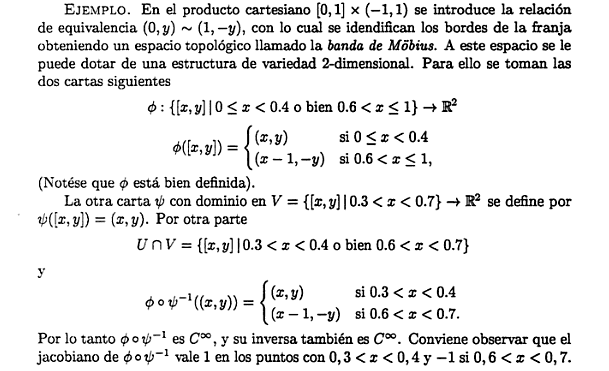
\includegraphics[keepaspectratio=true,width=\linewidth]{img/ejemplo_6.png}
\end{center}

Para dotar a un conjunto de estructura diferencial basta con encontrar un atlas para el cual se cumpla la definición de estructura diferencial sobre el conjunto dado.

Tomamos 8 cartas de la siguiente forma:
\begin{enumerate}
\item
\[\appl{\phi_1}{\{(x,y,z) \tq x\in [0,1), y \in [0,1), z \geq 0\}}{\real^3}\]
siendo $\phi_1=Id$
\item
\[\appl{\phi_2}{\{(x,y,z) \tq x\in (-1,0], y \in [0,1), z \geq 0\}}{\real^3}\]
siendo $\phi_2((x,y,z)=(-x,y,z)$
\item
\[\appl{\phi_3}{\{(x,y,z) \tq x\in [0,1), y \in (-1,0], z \geq 0\}}{\real^3}\]
siendo $\phi_3((x,y,z)=(x,-y,z)$
\item
\[\appl{\phi_4}{\{(x,y,z) \tq x\in [0,1), y \in [0,1), z < 0\}}{\real^3}\]
siendo $\phi_4((x,y,z)=(x,y,-z)$
\item
\[\appl{\phi_5}{\{(x,y,z) \tq x\in (-1,0], y \in (-1,0], z \geq 0\}}{\real^3}\]
siendo $\phi_5((x,y,z)=(-x,-y,z)$
\item
\[\appl{\phi_6}{\{(x,y,z) \tq x\in (-1,0], y \in [0,1), z < 0\}}{\real^3}\]
siendo $\phi_6((x,y,z)=(-x,y,-z)$
\item
\[\appl{\phi_7}{\{(x,y,z) \tq x\in [0,1), y \in (-1,0], z < 0\}}{\real^3}\]
siendo $\phi_7((x,y,z)=(x,-y,-z)$
\item
\[\appl{\phi_8}{\{(x,y,z) \tq x\in (-1,0], y \in (-1,0], z < 0\}}{\real^3}\]
siendo $\phi_8((x,y,z)=(-x,-y,-z)$

\end{enumerate}

La combinación de una de estas funciones con la inversa de otra no implicará más que cambios de signo sobre las variables de tal forma que
\[\phi_i\circ \inv{\phi_j}(x,y,z)=(\pm x, \pm y, \pm z\]
y queda claro que estas aplicaciones son $C^{\infty}$ y sus inversas, que son de la misma forma, también. Conviene observar que el jacobiano vale siempre $\pm 1$
\end{problem}

\section{fasc-4-ejemplos}

\subsection{Variedades}
\begin{problem}[2]
Estudiar, siguiendo el modelo de $S^2$ la estructura de variedad diferenciable, con dos cartas, en $S^n$

\solution
\textcolor{blue}{Hecho por Pedro. No fiarse al 100\%}

Comenzamos considerando una esfera de radio 1 en $\real^n$ que tendrá la ecuación:
\[\sum_{i=1}^n x_i^2=1\]
y describiendo explícitamente el atlas de dos cartas dado por la proyección estereográfica.

Siguiendo el ejemplo de la hoja, consideramos la proyección tomando el polo norte $(1,0...0)$ y el plano $x_1=-1$. Posteriormente construiremos la segunda carta tomando el polo sur $(-1,0...0)$ y el plano $x_1=1$. Vamos a ello.

\textbf{Primera carta}

\begin{itemize}
\item Supongamos un punto $p$ cualquiera del plano $x_1=-1$:
\[p=(-1,x_2,...x_n)\]

Si construimos la recta que lo une con el polo norte y la intersecamos con la esfera $S^n$ obtenemos el punto intersección $q$.
\[q = \left(1-2t, x_2\cdot t,...,x_n\cdot t\right)\]
Si el punto es la intersección con la esfera, su módulo deberá ser 1. Utilizamos este dato para calcular $t$.

\[1+4t^2-4t+t^2\left(\sum_{i=2}^nx_i^2\right)=1 \implies 4t^2-4t+t^2\left(\sum_{i=2}^nx_i^2\right) = 0 \implies t=\frac{4}{\sum_{i=2}^nx_i^2+4}\]

Por tanto el punto de intersección es:
\[q=\left(1-\frac{8}{\sum_{i=2}^nx_i^2+4}, \frac{4x_2}{\sum_{i=2}^nx_i^2+4},...,\frac{4x_n}{\sum_{i=2}^nx_i^2+4} \right)\]

\item Al revés. Empezamos ahora con un punto
\[x\in S^n\tq x=(α_1...α_n) \text{ con } \sum_{i=1}^n α_i^2 = 1\]

Construimos ahora el vector que une este punto con el polo norte y lo intersecamos con el plano $x_1=-1$

La recta unión con el polo norte queda de la forma:
\[\left(1+t(α_1+1),α_2t,...,α_nt \right)\]
y forzamos la intersección de esta recta con el plano para conocer el punto
\[1+t(α_1+1)=-1 \implies t = \frac{-2}{α_1+1}\]
con lo que el punto sería:
\[\left( -1, \frac{-2α_2}{α_1-1}, ..., \frac{-2α_n}{α_1-1}\right)=\left( -1, \frac{2α_2}{1-α_1}, ..., \frac{2α_n}{1-α_1}\right)\footnote{En el ejmplo de la hoja creo que escriben $α_1$ en función de las otras coordenadas, pero no veo necesaria esta complicación}\]
\end{itemize}

\textbf{Segunda carta}
\begin{itemize}
\item Supongamos un punto $p$ cualquiera del plano $x_1=1$:
\[p=(1,x_2,...x_n)\]

Si construimos la recta que lo une con el polo sur y la intersecamos con la esfera $S^n$ obtenemos el punto intersección $q$.
\[q = \left(-1+2t, x_2\cdot t,...,x_n\cdot t\right)\]
Si el punto es la intersección con la esfera, su módulo deberá ser 1. Utilizamos este dato para calcular $t$.

\[1+4t^2-4t+t^2\left(\sum_{i=2}^nx_i^2\right)=1 \implies 4t^2-4t+t^2\left(\sum_{i=2}^nx_i^2\right) = 0 \implies t=\frac{4}{\sum_{i=2}^nx_i^2+4}\]

Por tanto el punto de intersección es:
\[q=\left(-1+\frac{8}{\sum_{i=2}^nx_i^2+4}, \frac{4x_2}{\sum_{i=2}^nx_i^2+4},...,\frac{4x_n}{\sum_{i=2}^nx_i^2+4} \right)\]

\item Al revés. Empezamos ahora con un punto
\[x\in S^n\tq x=(α_1...α_n) \text{ con } \sum_{i=1}^n α_i^2 = 1\]

Construimos ahora el vector que une este punto con el polo sur y lo intersecamos con el plano $x_1=1$

La recta unión con el polo sur queda de la forma:
\[\left(-1+t(α_1+1),α_2t,...,α_nt \right)\]
y forzamos la intersección de esta recta con el plano para conocer el punto
\[-1+t(α_1+1)=1 \implies t = \frac{2}{α_1+1}\]
con lo que el punto sería:
\[\left( 1, \frac{-2α_2}{α_1+1}, ..., \frac{-2α_n}{α_1+1}\right))\]
\end{itemize}

Estudiamos ahora un punto cualquiera del plano $(-1,...x_n)$. Si lo mandamos en la esfera por la primera proyección que hemos calculado, llegamos al punto
\[\left(1-\frac{8}{\sum_{i=2}^nx_i^2+4}, \frac{4x_2}{\sum_{i=2}^nx_i^2+4},...,\frac{4x_n}{\sum_{i=2}^nx_i^2+4} \right)\]

Ahora calculamos la imagen directa de este punto por la segunda proyección estereográfica, con lo que llegamos a:
\[\left( 1, \frac{-2\frac{4x_2}{\sum_{i=2}^nx_i^2+4}}{2-\frac{8}{\sum_{i=2}^nx_i^2+4}}, ..., \frac{-2\frac{4x_n}{\sum_{i=2}^nx_i^2+4}}{2-\frac{8}{\sum_{i=2}^nx_i^2+4}}\right)=\left( 1, \frac{-4x_2}{\sum_{i=2}^nx_i^2},...,\frac{-4x_n}{\sum_{i=2}^nx_i^2}\right)\]

y podemos ver que se trata de un difeomorfismo sobre su imagen

\textcolor{blue}{En algún punto he metido la gamba con los signos porque debería salirme todo positivo. Pero ya he currado mucho con este ejercicio. Una paja y a seguir.}

\end{problem}



\begin{problem}[3]
Parametrizamos los puntos del hemisferio norte de la esfera $x_2 > 0$,
excluyendo el ecuador ($x_2 = 0$), en la forma $(θ, τ, + \sqrt{1 − θ^2 − τ^2})$ con
$θ^2 + τ^2 < 1$. Esto convierte al hemisferio norte en una carta coordenada, y podemos cubrir la esfera con seis cartas de este tipo tomando
como ecuador cada una de las intersecciones de la esfera con los planos
coordenados. COMPROBAR que, efectivamente, se trata de un atlas.

DEMOSTRAR que los dos atlas son equivalentes, viendo que los cambios
de carta de una carta de uno de ellos a una carta del otro inducen difeomorfismos.

\solution
\end{problem}

\begin{problem}[4]
Demostrar que no existe ninguna variedad diferenciable compacta que se pueda recubrir con una única carta coordenada
\solution

\textcolor{blue}{Hecho por mi. No fiarse al 100\%}

Si una variedad se puede recubrir por una única carta será homeomorfa a un abierto de $\real^n$ y, consecuentemente, nunca podrá ser compacta.

Esta respuestá está basada en la proposición 1.28 del documento: \href{http://ocw.um.es/ciencias/geometria-y-topologia/material-de-clase-1/01-variedadesdiferenciablessubvariedades-v100901.pdf}{Variedades Diferenciales y Subvariedades.pdf}
\end{problem}

\begin{problem}[5]
Demostrar que toda variedad 1-dimensional compacta y conexa es difeomorfa a la circunferencia $S^2$
\solution

\textcolor{blue}{Hecho por mi. No fiarse al 100\%}

Para empezar es obvio que en caso de haber un difeomorfismo entre una variedad y la circunferencia, la variedad ha de ser compacta y conexa, pues así lo es la circunferencia.

Para resolver este ejercicio me baso en la proposición \href{https://books.google.es/books?id=CAOjRFAMJFUC&pg=PA131&lpg=PA131&dq=variedad+1-dimensional&source=bl&ots=MLkMP7HMyo&sig=aLLSSaYknqPZhPsn-5jJM2MwPAc&hl=es&sa=X&ei=DeMeVZSOEczZPdLkgfgJ&ved=0CCcQ6AEwAQ#v=onepage&q&f=false}{VI.1.6}. Básicamente la copio como un bellaco pero ahí dejo el link para el que quiera profundizar.

\textcolor{blue}{Justo en la versión que se puede consultar gratis en Google han quitado las dos páginas clave en que salía esto. El lunes pillo el libro en ciencias y lo completo}

\end{problem}

\begin{problem}[6]
Demostrar, como consecuencia del teorema de invarianza del dominio, que si $n \neq m$, no pueden ser homeomorfos $\real^n$ y $\real^m$. Tampoco es posible que sean homeomorfos un abierto de $\real^n$ con uno de $\real^m$
\solution

\textcolor{blue}{Hecho por Pedro. No fiarse al 100\%}

La solución se ha obtenido de este \href{http://www.cmat.edu.uy/~rpotrie/documentos/pdfs/invarianciadimension.pdf}{documentopdf}

\textcolor{blue}{Esta demostración se hace prácticamente usando los conocimiento del curso de Topología y no veo una forma clara de hacerlo con lo estudiado en este curso de Geometría Diferencial.}
\end{problem}

\begin{problem}[7]
Demostrar que, si $\appl{f}{M}{N}$ es una función continua y localmente inyectiva de variedades topologícas de dimensión $n$, entonces la imagen de todo abierto $U \subset M$ es un abierto de $N$. En particular, $f(M)\subset N$ debe ser un abierto, que puede ser toda la variedad $N$
\solution

\textcolor{blue}{Hecho por Pedro. No fiarse al 100\%}

Esto es un resultado de Topología que no voy a rehacer ya que no le veo mucha relación con lo que estamos estudiando en esta asignatura.

Por comentar algo relacionado con lo que estamos viendo, he viso en Wikipedia, y cito textualmente: ``El teorema de la invariancia del dominio establece que una función continua y localmente inyectiva entre dos variedades topológicas n-dimensionales debe ser abierta.''
\end{problem}

\begin{problem}[8]
Sea $S$ el conjunto de sucesiones $\appl{σ}{\nat}{\real}$ de números reales.

Definimos una topología en $S$ exigiendo que todas las funciones naturales de proyección
\[\appl{μ_{i_1,i_2,...,i_n}}{S}{\real^n}\]
sean continuas.\footnote{Estas funciones básicamente llevan la sucesión a un vector de $\real^n$ formado por $n$ elementos de la sucesión.}

Definimos una función $\appl{F}{S}{S}$ mediante
\[F(x_0,x_1,...,x_n,...)=(x_1,x_2,...,x_n,...)\]
Demostrar que la función $F$ es continua e inyectia, pero su imagen no es un abierto de $S$

\solution


\end{problem}

\begin{problem}[9]
Sea $U$ una bola unidad abierta en $\real^n$. Comprobar que la aplicación
\[f(\vx)=\frac{\vx}{\sqrt{1-\norm{\vx}^2}}\]
es un difeomorfismo de $U$ en todo $\real^n$
\solution

\yoP

Para comprobar que $f$ es un difeomorfismo debemos ver que es diferenciable, biyectiva y con inversa diferenciable. Vamos a ello.

La función, descompuesta en coordenadas, queda de la forma:
\[f(\vx)=\left(\frac{x_1}{\sqrt{1-\norm{\vx}}}, \frac{x_2}{\sqrt{1-\norm{\vx}}}, ..., \frac{x_n}{\sqrt{1-\norm{\vx}}}\right)\]

Vamos a derivarla:
\[\frac{\partial f}{\partial x_i}=\left(\frac{x_1x_i}{(\sqrt{1-\norm{\vx}})^3},\frac{x_2x_i}{(\sqrt{1-\norm{\vx}})^3},..\frac{1}{\sqrt{1-\norm{\vx}}}+\frac{x_i^2}{(\sqrt{1-\norm{\vx}})^3}.,\frac{x_nx_i}{(\sqrt{1-\norm{\vx}})^3}\right)\]

Podemos observar que la derivada existe (y por tanto la función es diferenciable) en todo punto con norma distinta de 1. Puesto que nos estamos restringiendo a $U$ que es la bola unidad \textbf{abierta} no hay problema con esto.

Podemos ver de manera sencilla que la función es inyectvia pues la derivada nunca se anula y podemos ver que es sobreyectiva por contrucción. Para cualquier punto de $\real^n$ que tomemos podemos escribirlo como $f(\vx)$\footnote{Esto queda claro al calcular la función inversa, cosa que haremos a continuación}.

Por último nos queda estudiar la inversa.

\[f(\vx)=\vy \implies (y_1,....y_n)=\left(\frac{x_1}{\sqrt{1-\norm{\vx}}}, \frac{x_2}{\sqrt{1-\norm{\vx}}}, ..., \frac{x_n}{\sqrt{1-\norm{\vx}}}\right)\]

A ojo de buen cubero podemos ver que la función inversa sería
\[f^{-1}(\vy)=\frac{\vy}{\sqrt{1+\norm{\vy}}}\]
cosa que podemos comprobar fácilmente.

Resulta también trivial la observación de que esta función inversa también es diferenciable, por lo que queda claro que $f$ es un difeomorfismo.

\end{problem}


\subsection{Campos}
\begin{problem}[1]
(\textbf{Grupos uniparamétricos de automorfismos}) En cada uno de los siguientes ejemplos se da una familia uniparamétrica de automorfismos de $\real^n$ y se pide que se compruebe que es un grupo y determine el campo asociado (\textbf{generador infinitesimal del grupo}). En todos los casos el grupo es un grupo de transformaciones lineales y el campo es un campo lineal (coeficientes de grado a lo más uno)

\ppart Grupo de traslaciones
\[τ_1(x_1,...,x_n)=(x_1+t,x_2,...,x_n)\]

\ppart Grupo de homotecias
\[τ_t(x_1,...,x_n)=(e^tx_1, e^tx_2,...,e^tx_n\]

\ppart Sea $A$ una matriz $n\times n$. Definimo un grupo uniparamétrico de automorfismos, asociado a la matriz $A$, mediante
\[τ_t(X)=e^{tA}X\]
¿Es el primer ejemplo un caso particular de este?

\ppart
Supongamos ahora $n=2$, y sea
\[ \left( \begin{array}{cc}

\cos(t) & -\sin(t) \\
\sin(t) & \cos(t)

\end{array} \right)\]
la matriz de una rotación de ángulo variable $t$ en el plano. Definimos un grupo uniparamétrico de automorfismos
\[τ_t(x_1,x_2)=A(t)\cdot {x_1 \choose x_2}\]

¿Es este ejemplo un caso particular del c)?

\solution
\yoP

Para demostrar que cada uno de estos conjuntos es un grupo debemos identificar la operación que define el grupo, demostrar que es asociativa y encontrar el elemento neutro o identidad y el inverso.

\spart
La operación suma se define de la siguiente forma:
\[(τ_a+τ_b)(x_1,...,x_n)=(x_1+a+b,x_2,...,x_n)\]

Es evidente que la operación es asociativa, el elemento neutro es $τ_0$ y el inverso de $τ_t$ es $τ_{-t}$

Queda claro que es un grupo.

Vamos a encontrar el campo asociado. La teoría de lo que vamos a hacer a continuación viene en las páginas 73-74 de \href{http://matematicas.unex.es/~ricarfr/EcDiferenciales/LibroEDLat.pdf}{documento.pdf}

Básicamente nos da un teorema y su demostración. El teorema dice:

Sea $X$ un grupo uniparamétrico local de clase $k$. Para cada $f\in C^{\infty}(U)$ y $p \in U$ definimos
\[(Df)(p)=\lim_{t \to 0}\frac{f[X(t,p)]-f(p)}{t}\]
entonces $D \in D_k(U)$ y lo llamaremos generador infinitesimal de X.

El ejemplo concreto que vamos a hacer (o uno muy similar) así como los siguientes vienen resuletos al final de la página 16 de \href{http://matematicas.unex.es/~ricarfr/EcDiferenciales/LibroEDLat.pdf}{documento.pdf}

Así para este ejemplo tendríamos la aplicación flujo $\appl{\phi}{\real^{n+1}}{\real^n}$ siendo $\phi(x_1,...,x_n,t)=(x_1+t,x_2,...,x_n)$.

\[X = \left(\frac{\partial \phi}{\partial t}\right)_{t=0} \frac{\partial}{\partial x_i}=\frac{\partial}{\partial x}\]


\textbf{Del último documento mencionado cabe destacar:}

\begin{defn}[Generador infinitesimal]
Sea $\{σ_t\}$ un grupo monoparamétrico de transformaciones de U. Llamamos \textbf{generador infinitesimal} de $\{σ_t\}$ al campo vectorial que asigna al punto $p$, el vector tangente a la curva $(-ε,ε)\to U$, $t \to σ_t(p)$

Consideremos $\appl{\phi}{\real \times U}{U}$ la aplicación flujo del grupo $\phi(t,p)=σ_t(p)$. entonces el generador infinitesimal puede considerarse
\[X = \sum_{i=1}^n \left( \frac{\partial \phi_i}{\partial t}\right)_{t=0}\frac{\partial}{\partial x_i}\]
\end{defn}

\end{problem}

\begin{problem}[2]
Sea $D$ el campo en $\real^2$ definido como
\[D=x \frac{\partial}{\partial x}+y \frac{\partial}{\partial y }\]

El campo está definido en tdo el plano pero

\ppart Una integral primera definida en todo el plano es necesariamente constante

\ppart Para cada punto, diferente al origen hay un entorno en el que hay una integral primera. Determnar todas esas integrales primeras no globales y los abiertos máximos en que están definidas.
\solution
\end{problem}

\begin{problem}[3]
Estudiar el campo en el plano definido como
\[D=(y+x(1-x^2-y^2))\frac{\partial}{\partial x} + (-x+y(1-x^2-y^2))\frac{\partial}{\partial y}\]
usando, si te parece conveniente, un cambio a coordenadas polares.
\solution

\end{problem}


\chapter{Discusiones interesantes}

\section{Funciones suaves no analíticas}

\begin{figure}[hbtp]
\centering
\inputtikz{Ap_SuaveNoAnalitica}
\caption{Una función suave no analítica, dada por $f(x) = 0$ cuando $x ≤ 0$ y $f(x) = e^{\frac{-1}{x}}$ cuando $x > 0$. $f$ se anula en el origen y todas sus derivadas también, pero $f$ no es nula.}
\end{figure}

En la sección \fref{sec:DimTangente} hablábamos de anillos, y surge la pregunta de si esos anillos de funciones son también dominios. No lo son por la existencia de divisores de cero: funciones suaves no analíticas.

Estas funciones son $C^∞$ con $f^{(n)}(x) = 0\; ∀n$, pero $f ≠ 0$, una contradicción aparente ya que su desarrollo de Taylor con todas las derivadas nulas sería idénticamente nulo.

En Wikipedia \href{http://en.wikipedia.org/wiki/Non-analytic_smooth_function}{hay una discusión más detallada sobre este tema}.

\section{Espacios con distintas estructuras no difeomorfas}
\label{sec:MismoEspacioNoDifeomorfo}

Algo bastante contraintuitivo es que puede haber diferentes estructuras para un espacio que no son difeomorfas. En 1983, se probó que $ℝ^4$ tiene infinitas estructuras diferenciables no difeomorfas entre sí.

Este resultado parte de algo que ya se sabía, que es lo que ocurre en el caso de las esferas en dimensiones altas, por ejemplo. En \href{http://plus.maths.org/content/richard-elwes}{este artículo tienen una introducción al tema}, y aquí está el \href{http://projecteuclid.org/euclid.bams/1183550021}{artículo de 1983 de Simon Donaldson}.

\section{Formas diferenciales y factores integrantes}

Podemos relacionar formas diferenciales con los factores integrantes que veíamos en cursos de EDOs. Si tenemos \[ ω = M(x,y) \dif x + N(x,y) \dif y \] en un dominio contráctil, entonces $\dif ω = 0$ implica que $ω = \dif f$ para alguna función $f$. Si la ecuación $f = cte$ define una curva γ, entonces se cumple $\restr{ω}{γ} = 0$ y por lo tanto se puede resovler la curva con la ecuación diferencial \[ \deriv{y}{x} = - \frac{M}{N} \]

Si no tenemos que $\dif ω = 0$, sí podemos tratar de resolver $\dif (μω) = 0$ donde $μ$ es un factor integrante. En ese caso, el problema puede ser equivalente a resolver $μω=\dif f$. Para algunos casos particulares se sabe que el factor integrante sólo depende de una variable, lo que permite calcular explícitamente μ a partir de $\dif (μω) = 0$.


\chapter{Definiciones adicionales}

\begin{defn}[Delta\IS de Kronecker] \label{def:DeltaKronecker} La delta de Kronecker se define como \[ δ_{ij} = \begin{cases} 0 & i ≠ j \\ 1 & i = j \end{cases} \] \end{defn}

\section{Análisis Matemático}

\begin{theorem} [Teorema\IS de la función inversa] \label{thm:FuncionInversa} Sea $\appl{F}{\Omega\subset\real^N}{\real^N} \text{ con } F\in C^1(\Omega)$.

Supongamos $DF(\ga)$ invertible, $\ga \in \Omega$. Entonces existe un abierto $V \tlq F(\ga)\in V$, un abierto $U \tlq \ga \in U$ y una inversa local $\appl{G}{V}{U}$. Además, $G$ es diferenciable en $U$ y

\[ DG(y) = \left[DF(\F(y))\right]^{-1}, \forall y \in U \]
\end{theorem}

\begin{theorem}[Teorema\IS de la función implícita] \label{thm:FuncionImplicita} Dadas $n$ ecuaciones, $n+m$ incógnitas, consideramos

$$\appl{F}{\Omega\subset\underbrace{\real^M}_{x,y} \times \underbrace{\real^N}_{z}}{\real^N}$$

Supongamos $F\in C^1$. Sea $\ga \in \real^M, \gor{b} \in \real^N \tlq (\gor{a},\gor{b})\in \Omega , F(a,b)=0$. Supongamos $D_yF(\ga,\gb)$ no singular, $\det(D_yF)\neq 0$. Entonces existen abiertos $\omega \subset \real^M, \Theta \in\real^n$, con $\ga \in \omega, \gb \in \Theta$ y una única función: \[ \appl{g}{\omega\subset\real^M}{\Theta \subset\real^N}, g\in C^1(\omega) \]

que cumple

\[ g(\ga) = \gb;\; F(\gx,g(\gx)) = \gor{0}\; \forall \gx \in \omega \]
\[ Dg(\gx) = - \left[D_yF(\gx,g(\gx))\right]^{-1} \cdot D_xF(\gx,g(\gx)) \]
\end{theorem}

\begin{defn}[Difeomorfismo] Se dice que $\appl{F}{A}{B}$ es difeomorfismo si es biyectiva, derivable y con inversa derivable. \label{def:Difeomorfismo}
\end{defn}

\begin{defn}[Homeomorfismo] Se dice que una función $\appl{f}{X}{Y}$ entre dos espacios es un homeomorfismo si es biyectiva, continua y con inversa continua. \label{def:Homeomorfismo}
\end{defn}

\section{Espacio vectorial libre}
\label{sec:EspacioVectorialLibre}

La idea del espacio vectorial libre es generalizar de alguna forma los espacios vectoriales y darles una construcción más abstracta. Tomemos, por ejemplo, $\vv ∈ ℝ^2$. Normalmente lo escribiríamos como combinación lineal de elementos de la base, o como coordenadas $(3,4)$, por ejemplo. Sin embargo, hay otra forma de verlo, y es como una función que para cada coordenada nos da su valor. Es decir, que podemos definir una función $\appl{f_\vv}{\set{1,2}}{ℝ}$ con las coordenadas $f_\vv(1) = 3, f_\vv(2) = 4$.

Ahora bien, esta definición requiere que tengamos en cuenta los elementos de la base. No nos vale de nada hablar de la primera coordenada si no sabemos cuáles son los elementos de la base. Lo que haremos será generalizar el dominio de esa función y hacer que sea la base. Esto es, si $\base = \set{e_1, e_2}$ es la base de $ℝ^2$, simplemente definiremos $\appl{f_\vv}{\base}{ℝ}$ con las coordenadas $f_\vv(e_1) = 3, f_\vv(e_2) = 4$.

¿Podemos generalizar esto a cualquier conjunto en lugar de la base? Esto es, ¿qué ocurre si tomamos los elementos del espacio vectorial libre como funciones $\appl{f}{X}{\kbb}$ con $X$ un conjunto arbitrario y $\kbb$ un cuerpo?

Lo que ocurre es que tenemos igualmente un espacio vectorial, con operaciones bien definidas. Vamos a definirlo estrictamente:

\begin{defn}[Espacio\IS vectorial libre]
Dado $X$ un conjunto y $\kbb$ un cuerpo, se define el espacio vectorial libre $\kbb^X$ como \[ \kbb^X ≝ \set{\appl{f}{X}{\kbb} \tq \card{\inv{f}\left(\kbb \setminus \set{0}\right)} < ∞ }\] es decir, las funciones que no son nulas sólo en una cantidad finita de elementos de $X$ (no queremos vectores con infinitas coordenadas).
\end{defn}

Resulta que ese conjunto $\kbb^X$ tiene bien definidas las operaciones de suma y producto por escalar de forma bastante obvia.

\nocite{doCarmo94,chamizo07,bryan,diaz03,barden03,crossley10}

\bibliography{../Apuntes}{}

\printindex
\end{document}
